% User guide for the cronologic GmbH & Co. KG TimeTagger4 and xTDC4 boards.
%
% to create user guides with the correct filenames run the parent configuration files like this
% pdflatex xTDC4_User_Guide.tex
% pdflatex TimeTagger4_User_Guide.tex
% 
% Visit www.cronologic.de for ready made PDFs of these user guides
% https://www.cronologic.de/products/tdcs/xtdc4-pcie 
% https://www.cronologic.de/products/tdcs/timetagger
%
% You can contribute to this documentation at
% https://github.com/cronologic-de/ug_xtdc4_timetagger
%
% the whole user guide is provided by cronologic GmbH & Co. KG under a
% Creative Commons Attribution-NoDerivatices 4.0 International License
% https://creativecommons.org/licenses/by-nd/4.0/
% except fpr extraplaceins.sty which is in the public domain

% configure Visual Studio Code LaTeX Workshop 
% !TEX root = xHPTDC8_User_guide.tex
  
\documentclass[11pt,notitlepage]{scrreprt}
\usepackage{cronologicug}

% this file creates two similar user guides depending on the commend \deviceName
 
%source files that differ between versions can be input with \ttinput
%this will prefix the include with TT4_ or xTDC4, depending on versoin

\usepackage{ifthen}
% instead of setting \devicename in a top level file you can also provide it at the command line
% pdflatex "\newcommand{\deviceName}{xTDC4} % User guide for the cronologic GmbH & Co. KG TimeTagger4 and xTDC4 boards.
%
% to create user guides with the correct filenames run the parent configuration files like this
% pdflatex xTDC4_User_Guide.tex
% pdflatex TimeTagger4_User_Guide.tex
% 
% Visit www.cronologic.de for ready made PDFs of these user guides
% https://www.cronologic.de/products/tdcs/xtdc4-pcie 
% https://www.cronologic.de/products/tdcs/timetagger
%
% You can contribute to this documentation at
% https://github.com/cronologic-de/ug_xtdc4_timetagger
%
% the whole user guide is provided by cronologic GmbH & Co. KG under a
% Creative Commons Attribution-NoDerivatices 4.0 International License
% https://creativecommons.org/licenses/by-nd/4.0/
% except fpr extraplaceins.sty which is in the public domain

% configure Visual Studio Code LaTeX Workshop 
% !TEX root = xHPTDC8_User_guide.tex
  
\documentclass[11pt,notitlepage]{scrreprt}
\usepackage{cronologicug}

% this file creates two similar user guides depending on the commend \deviceName
 
%source files that differ between versions can be input with \ttinput
%this will prefix the include with TT4_ or xTDC4, depending on versoin

\usepackage{ifthen}
% instead of setting \devicename in a top level file you can also provide it at the command line
% pdflatex "\newcommand{\deviceName}{xTDC4} % User guide for the cronologic GmbH & Co. KG TimeTagger4 and xTDC4 boards.
%
% to create user guides with the correct filenames run the parent configuration files like this
% pdflatex xTDC4_User_Guide.tex
% pdflatex TimeTagger4_User_Guide.tex
% 
% Visit www.cronologic.de for ready made PDFs of these user guides
% https://www.cronologic.de/products/tdcs/xtdc4-pcie 
% https://www.cronologic.de/products/tdcs/timetagger
%
% You can contribute to this documentation at
% https://github.com/cronologic-de/ug_xtdc4_timetagger
%
% the whole user guide is provided by cronologic GmbH & Co. KG under a
% Creative Commons Attribution-NoDerivatices 4.0 International License
% https://creativecommons.org/licenses/by-nd/4.0/
% except fpr extraplaceins.sty which is in the public domain

% configure Visual Studio Code LaTeX Workshop 
% !TEX root = xHPTDC8_User_guide.tex
  
\documentclass[11pt,notitlepage]{scrreprt}
\usepackage{cronologicug}

% this file creates two similar user guides depending on the commend \deviceName
 
%source files that differ between versions can be input with \ttinput
%this will prefix the include with TT4_ or xTDC4, depending on versoin

\usepackage{ifthen}
% instead of setting \devicename in a top level file you can also provide it at the command line
% pdflatex "\newcommand{\deviceName}{xTDC4} % User guide for the cronologic GmbH & Co. KG TimeTagger4 and xTDC4 boards.
%
% to create user guides with the correct filenames run the parent configuration files like this
% pdflatex xTDC4_User_Guide.tex
% pdflatex TimeTagger4_User_Guide.tex
% 
% Visit www.cronologic.de for ready made PDFs of these user guides
% https://www.cronologic.de/products/tdcs/xtdc4-pcie 
% https://www.cronologic.de/products/tdcs/timetagger
%
% You can contribute to this documentation at
% https://github.com/cronologic-de/ug_xtdc4_timetagger
%
% the whole user guide is provided by cronologic GmbH & Co. KG under a
% Creative Commons Attribution-NoDerivatices 4.0 International License
% https://creativecommons.org/licenses/by-nd/4.0/
% except fpr extraplaceins.sty which is in the public domain

% configure Visual Studio Code LaTeX Workshop 
% !TEX root = xHPTDC8_User_guide.tex
  
\documentclass[11pt,notitlepage]{scrreprt}
\usepackage{cronologicug}

% this file creates two similar user guides depending on the commend \deviceName
 
%source files that differ between versions can be input with \ttinput
%this will prefix the include with TT4_ or xTDC4, depending on versoin

\usepackage{ifthen}
% instead of setting \devicename in a top level file you can also provide it at the command line
% pdflatex "\newcommand{\deviceName}{xTDC4} \input{User_Guide.tex}"

% or define it here
%\newcommand{\deviceName}{TimeTagger4}
%\newcommand{\deviceName}{xTDC4}

  
\ifthenelse{\isundefined{\deviceName}}{ 
	\message {\\ WARNING: Undefined device name, TimeTagger4 used}
	\newcommand{\deviceName}{TimeTagger4}}{}
\message{\\Device name is \deviceName }


%output the first option for the TimeTagger, the second one otherwise
% example: 
% \itett{THIS IS A TimeTagger4}{THIS IS NOT}
\ifthenelse{\equal{\deviceName}{TimeTagger4}}{\newcommand{\itett}[2]{#1}}{\newcommand{\itett}[2]{#2}}
\itett{\message{\\TIMETAGGER\\}}{\message{\\NO TIMETAGGER\\}}

% output code only for the xHPTDC8 
% example: 
% \ifXHPTDC{THIS IS AN xHPTDC8} {THIS IS NOT}
% NOTE: Macro names may not contain digits
\ifthenelse{\equal{\deviceName}{xHPTDC8}} {\newcommand{\ifxHPTDC}[2]{#1}}{\newcommand{\ifxHPTDC}[2]{#2}}
\ifxHPTDC{\message{\\XHPTDC8\\}}{\message{\\NO XHPTDC\\}}
 
  
 
% output code for the TimeTagger4, xTDC4 or xHPTDC8
% example: 
% \txh{THIS IS A TimeTagger4}{THIS IS AN xTDC4}{THIS IS AN xHPTDC8}
\itett{\newcommand{\txh}[3]{#1}}{\ifxHPTDC{\newcommand{\txh}[3]{#3}} {\newcommand{\txh}[3]{#2}}}
 
\txh{ % TimeTagger4
	\message{Generating User Guide for TimeTagger4}
	\newcommand{\ttinput}[1]{\input{timetagger/#1}}
	\newcommand{\titlefile}{"figures/TT4_title.pdf"}
	\newcommand{\prefix}{timetagger4\tu}
	\newcommand{\PREFIX}{TIMETAGGER4\tu}
}{ % xTDC4
	\message{Generating User Guide for xTDC4}
	\newcommand{\ttinput}[1]{\input{xtdc/#1}}
	\newcommand{\titlefile}{"figures/xTDC4_title.pdf"}
	\newcommand{\prefix}{xtdc4\tu} 
	\newcommand{\PREFIX}{XTDC4\tu}
} 
{ % xHPTDC8
	\message{Generating User Guide for xHPTDC8}
	\newcommand{\ttinput}[1]{\input{xhptdc/#1}}
	\newcommand{\titlefile}{"figures/xHPTDC8_title.pdf"}
	\newcommand{\prefix}{xhptdc8\tu}
	\newcommand{\PREFIX}{XHPTDC8\tu}
} 

\hyphenation{Time-Tagger xTDC xHPTDC cronologic}


\newcommand{\ttvar}[2]{\noindent\textsf{\textbf{\textcolor{crongrey}{#1} \prefix #2}}}%for variable declaration
\newcommand{\ttdef}[1]{\noindent\textsf{\textcolor{crongrey}{\#{}define} \PREFIX #1}}%for definitions

\newcommand{\ugrev}{{1.8.0\tu draft\tu 6}}
%%%%%%%%%%%%%%%%%%%%%%%%%%%%%%%%%
 
\begin{document}  
\cronofront{\titlefile}
 
% 
	\chapter{Introduction}
		\ttinput{Intro.tex}

	\chapter{Hardware}  
		\input{common/Hardware.tex}

	\chapter{\deviceName\ Functionality}
		\input{common/Functionality.tex} 
		\input{common/Grouping.tex}
		\input{common/AutoTiger.tex} 

	\chapter{Driver Programming API\label{cp:api}} 
		% also includes common/StructConfig.tex and common/InfoStructs.tex
		\input{common/API.tex}  
		  
	\chapter{Run Time Control\label{cp:readout}}  % and packet format
		\ifxHPTDC{
			\input{xhptdc/Readout.tex}
		}{
			\input{common/Readout.tex}
		} 

	\chapter{Output Data Format\label{cp:packetformat}} 
		\ifxHPTDC{
			\input{xhptdc/PackForm.tex} 
		}{
			\input{common/PackForm.tex}
		}  
 
	\chapter{C Example}  
		\input{common/CExample.tex}

	\chapter{Technical Data}    
		\ttinput{Tech.tex} 
		\input{common/DIN.tex}

	\chapter{Revision History} 
		\noindent
		User Guide \hyperlink{ugrev}{\ugrev} as of 2020-02-04\\
		\\
		cronologic GmbH \& Co. KG\\
		Jahnstraße 49\\
		60318 Frankfurt am Main\\Germany\\
		\ttinput{FwRev.tex}
		\ifxHPTDC{\input{xhptdc/DrvRev.tex}}{\input{common/DrvRev.tex}} 
		\input{common/UGRev.tex}
\end{document}  "

% or define it here
%\newcommand{\deviceName}{TimeTagger4}
%\newcommand{\deviceName}{xTDC4}

  
\ifthenelse{\isundefined{\deviceName}}{ 
	\message {\\ WARNING: Undefined device name, TimeTagger4 used}
	\newcommand{\deviceName}{TimeTagger4}}{}
\message{\\Device name is \deviceName }


%output the first option for the TimeTagger, the second one otherwise
% example: 
% \itett{THIS IS A TimeTagger4}{THIS IS NOT}
\ifthenelse{\equal{\deviceName}{TimeTagger4}}{\newcommand{\itett}[2]{#1}}{\newcommand{\itett}[2]{#2}}
\itett{\message{\\TIMETAGGER\\}}{\message{\\NO TIMETAGGER\\}}

% output code only for the xHPTDC8 
% example: 
% \ifXHPTDC{THIS IS AN xHPTDC8} {THIS IS NOT}
% NOTE: Macro names may not contain digits
\ifthenelse{\equal{\deviceName}{xHPTDC8}} {\newcommand{\ifxHPTDC}[2]{#1}}{\newcommand{\ifxHPTDC}[2]{#2}}
\ifxHPTDC{\message{\\XHPTDC8\\}}{\message{\\NO XHPTDC\\}}
 
  
 
% output code for the TimeTagger4, xTDC4 or xHPTDC8
% example: 
% \txh{THIS IS A TimeTagger4}{THIS IS AN xTDC4}{THIS IS AN xHPTDC8}
\itett{\newcommand{\txh}[3]{#1}}{\ifxHPTDC{\newcommand{\txh}[3]{#3}} {\newcommand{\txh}[3]{#2}}}
 
\txh{ % TimeTagger4
	\message{Generating User Guide for TimeTagger4}
	\newcommand{\ttinput}[1]{\input{timetagger/#1}}
	\newcommand{\titlefile}{"figures/TT4_title.pdf"}
	\newcommand{\prefix}{timetagger4\tu}
	\newcommand{\PREFIX}{TIMETAGGER4\tu}
}{ % xTDC4
	\message{Generating User Guide for xTDC4}
	\newcommand{\ttinput}[1]{\input{xtdc/#1}}
	\newcommand{\titlefile}{"figures/xTDC4_title.pdf"}
	\newcommand{\prefix}{xtdc4\tu} 
	\newcommand{\PREFIX}{XTDC4\tu}
} 
{ % xHPTDC8
	\message{Generating User Guide for xHPTDC8}
	\newcommand{\ttinput}[1]{\input{xhptdc/#1}}
	\newcommand{\titlefile}{"figures/xHPTDC8_title.pdf"}
	\newcommand{\prefix}{xhptdc8\tu}
	\newcommand{\PREFIX}{XHPTDC8\tu}
} 

\hyphenation{Time-Tagger xTDC xHPTDC cronologic}


\newcommand{\ttvar}[2]{\noindent\textsf{\textbf{\textcolor{crongrey}{#1} \prefix #2}}}%for variable declaration
\newcommand{\ttdef}[1]{\noindent\textsf{\textcolor{crongrey}{\#{}define} \PREFIX #1}}%for definitions

\newcommand{\ugrev}{{1.8.0\tu draft\tu 6}}
%%%%%%%%%%%%%%%%%%%%%%%%%%%%%%%%%
 
\begin{document}  
\cronofront{\titlefile}
 
% 
	\chapter{Introduction}
		\ttinput{Intro.tex}

	\chapter{Hardware}  
		\section{Installing the Board}
The \deviceName\ board can be installed in any PCIe-CEM slot with x1 or more lanes. 
Make sure the PC is powered off and the main power connector is disconnected while installing the board.\par

%
\section{\deviceName\ Inputs and Connectors}
	Figure \ref{fig:bracket} shows the location of the inputs on the slot bracket.
%
	\begin{figure*}[hb]
		\begin{center}
			\ifxHPTDC{
				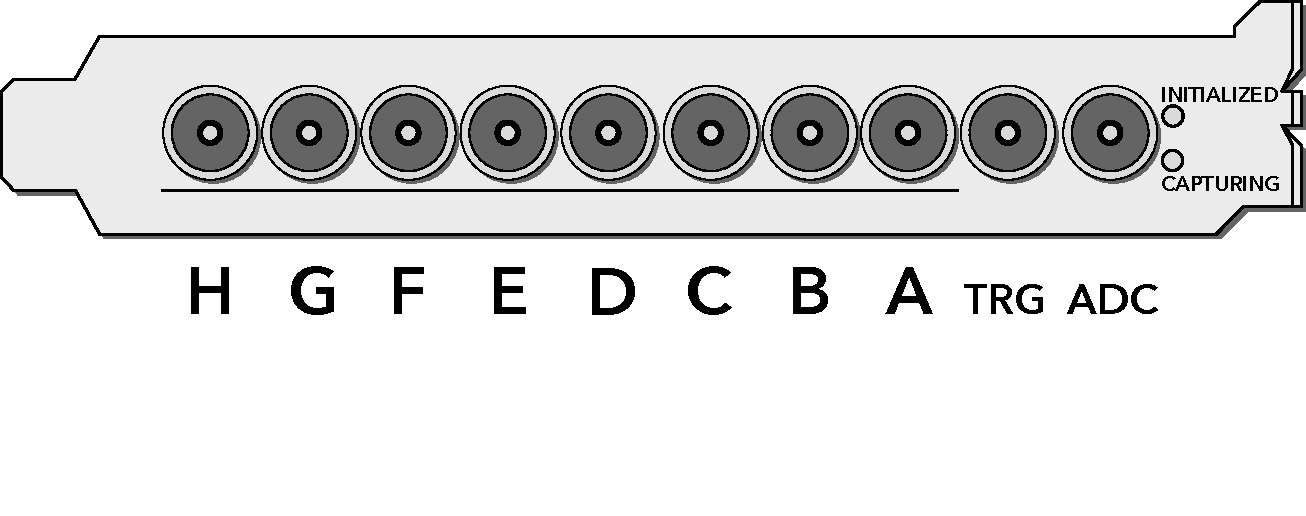
\includegraphics[width=0.6\textwidth]{figures/xHPTDC8_Slotblende.pdf}
			}{
				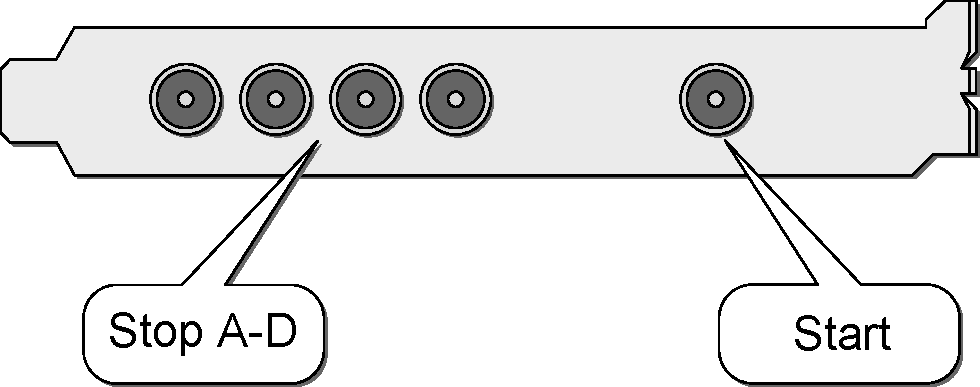
\includegraphics[width=0.6\textwidth]{figures/xTDC4_Slotblende.pdf}
			}
			\caption{Input connectors of the \deviceName\ on the PCIe bracket.\label{fig:bracket}}
		\end{center}
	\end{figure*}
	%
	\begin{figure*}[hb]
		\begin{center}
			\ifxHPTDC{
				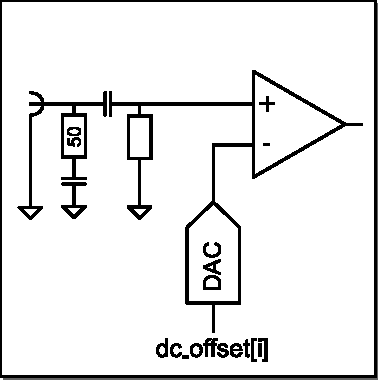
\includegraphics[width=0.3\textwidth]{xhptdc/figures/InputCircuit.pdf}
			}{
				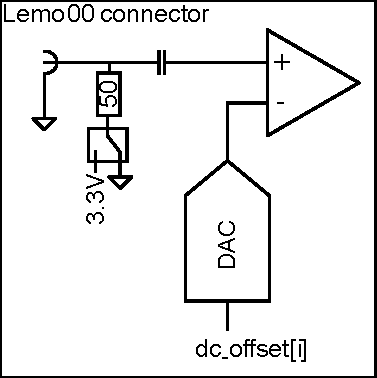
\includegraphics[width=0.3\textwidth]{figures/InputCircuit.pdf}
			}
			\caption{Input circuit for each of the input channels.\label{fig:inputcirc}}
		\end{center}
	\end{figure*}
	%

	Lemo-00 connectors are used for input connection. The inputs are AC-coupled and have an impedance of 50$\Omega$. 
	A schematic of the input circuit is shown in Figure \ref{fig:inputcirc}. 
	The digital threshold for any input can be adjusted to comply with a multitude of single ended signaling standards.
	The threshold can also be used to configure the input for either positive or negative pulses.
	
	
	The connectors can also be used as outputs. 
	\ifxHPTDC{AC-coupled}{DC-coupled} output pulses for automatic internal triggering and control of external devices 
	can be generated using the TiGer timing pattern generator. See section \ref{cp:tiger} for details on TiGer. 
	%
		\begin{figure*}[ht]
			\begin{center}
				\ifxHPTDC{
					\includegraphics[width=0.7\textwidth]{xhptdc/figures/xHPTDC8_schematic.pdf}
				}{
					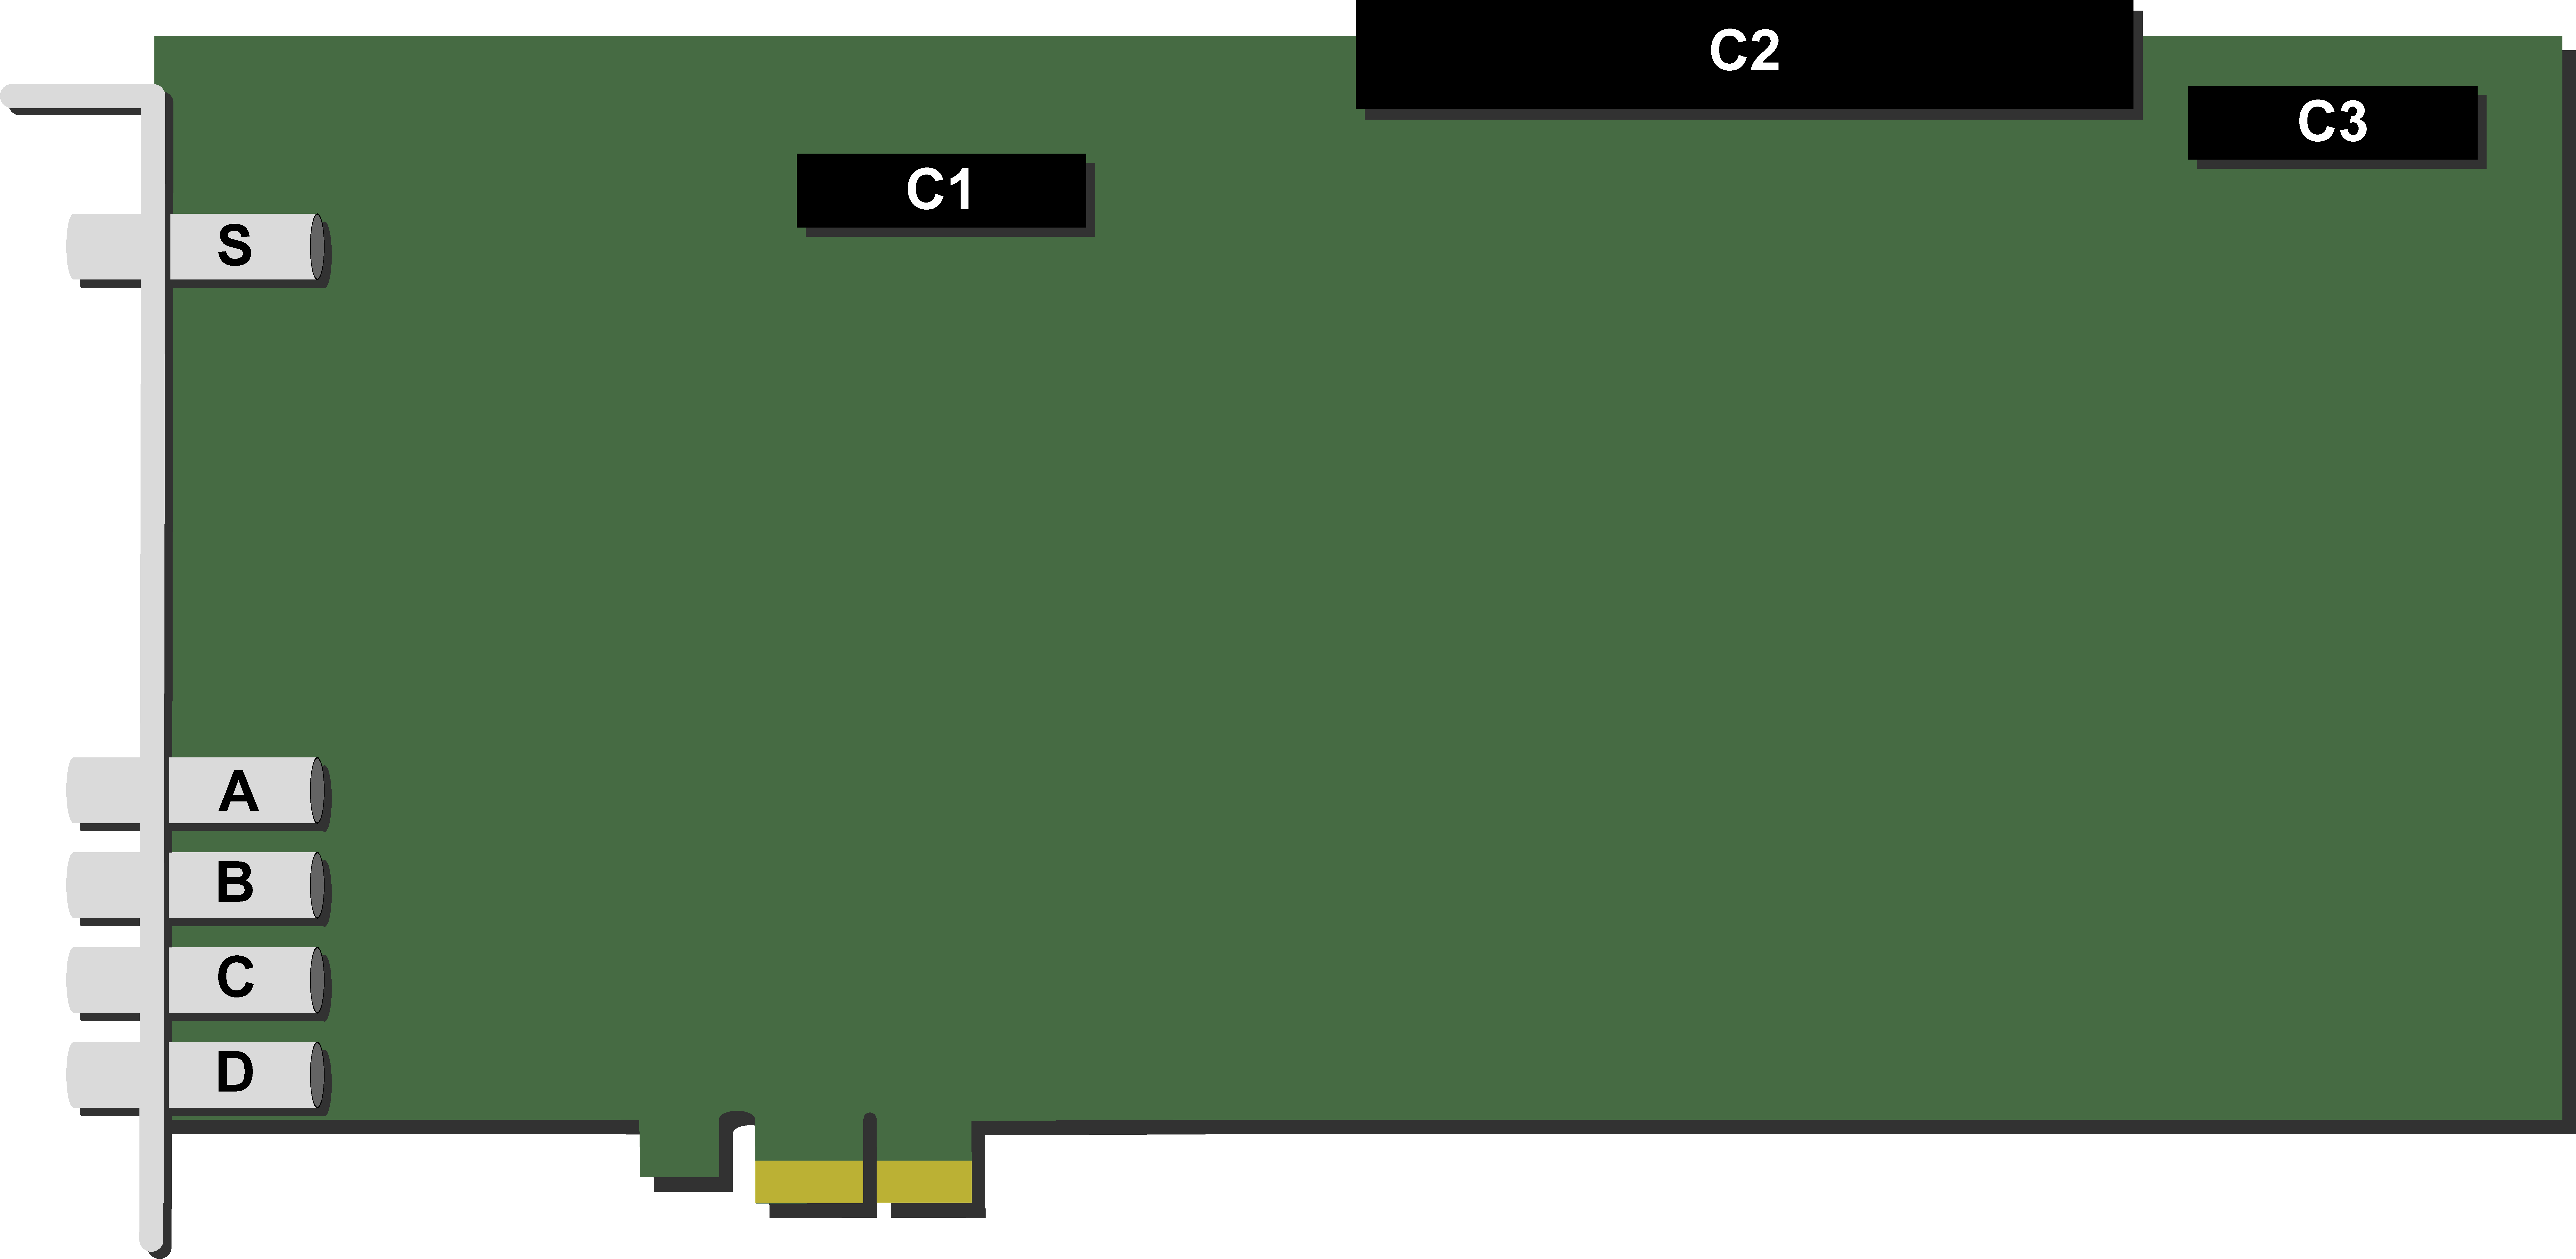
\includegraphics[width=0.7\textwidth]{figures/xTDC4_schematic.pdf}
				}
				
				\caption{Schematic view of a \deviceName\ board showing the inter-board connectors.\label{fig:schematics}}
			\end{center} 
		\end{figure*}
	%

	Furthermore, three inter-board connectors can be found at the top edge of the \deviceName\ board, 
	as displayed in Figure \ref{fig:schematics}. 
	Connector J25 is reserved for future use. The pinout of connector J12 is shown in Table \ref{J12} and the pinout of connector J6 is depicted in Table \ref{J6}.
	\ifxHPTDC{Connector J2 is a coax clock input that must receive a 10 MHz clock if multiple boards are used in together as described in section \ref{multiboard}.}{}

	\begin{table}
	\begin{small}
		\begin{center}
			\begin{tabular}{|c|c|}
				\hline
				Pin & Name\\
				\hline\hline
				1, 2 & GND\\
				\hline
				3, 4 & external CLK in N, external CLK in P\\
				\hline
				5, 6 & GND\\
				\hline
				7, 8 & reserved/NC\\
				\hline
				9, 10 & GND\\
				\hline
				11, 12 & reserved/NC\\
				\hline
				13, 14 & GND\\
				\hline
				15, 16 & reserved/NC\\
				\hline
				17, 18 & GND\\
				\hline
				19, 20 & reserved/NC\\
				\hline
				21, 22 & GND\\
				\hline
				23, 24 & reserved/NC\\
				\hline
				25, 26 & GND\\
				\hline
				27, 28 & reserved/NC\\
				\hline
				29, 30 & GND\\
				\hline
				31, 32 & reserved/NC\\
				\hline
				33, 34 & GND\\
				\hline
			\end{tabular}
			\caption{Pinout of connector J12.}
			\label{J12}
		\end{center}
	\end{small}
	\end{table}

	\begin{table}
	\begin{small}
		\begin{center}
			\begin{tabular}{|c|c|}
				\hline
				Pin & Name\\
				\hline\hline
				1 & +3.3 V\\
				\hline
				2 - 9 & reserved/NC\\
				\hline
				10 & GND\\
				\hline
			\end{tabular}
			\caption{Pinout of connector J6.}
			\label{J6}
		\end{center}
	\end{small}
	\end{table}

%%%%%%%%%%%%%%% multiboard
\ifxHPTDC{
	\section{Synchronizing multiple boards}
		\label{multiboard}
		If more than eight TDC inputs are required, up to eight boards can be synchronises within a system. 
		
		The \deviceName\ API described in chapter \ref{cp:api} manages up to eight boards automatically
		and provides a single data stream that contains sorted hit data from all boards in chronological order. 
		Channel A of each board is assigned channel number \textsf{board\tu index} $\cdot 10$. 
		The \textsf{board\tu index} is assigned to the boards in the order of the serial numbers starting at 0.

		\subsection{Connecting multiple boards}
			The boards must each receive a common 10~MHz clock on connector J2. The connector is inside the PC enclosure. 
			Connectors J12 of all boards must be connected with a flat band cable with a terminator at each end. 
			Cable and Terminator are available from cronologic. See figure \ref{fig:multiboard} for a wiring example.
			%
			\begin{figure*}[ht]
				\begin{center}
					\includegraphics[width=1\textwidth]{xhptdc/figures/multiboard.pdf}				
					\caption{Synchronising multiple boards with a ClockBox.\label{fig:multiboard}}
				\end{center} 
			\end{figure*}
			%
		\subsection{ClockBox}
			For systems of up to four boards cronologic offers the ClockBox product that conveniently makes four clock signals evailable 
			inside the PC enclosure. For use with the \deviceName, jumper JP3 of the CLockBox must be set as shown in Figure \ref{fig:clockbox} to set the clock frequency to 10~MHz. 
			%
			\begin{figure*}[ht]
				\begin{center}
					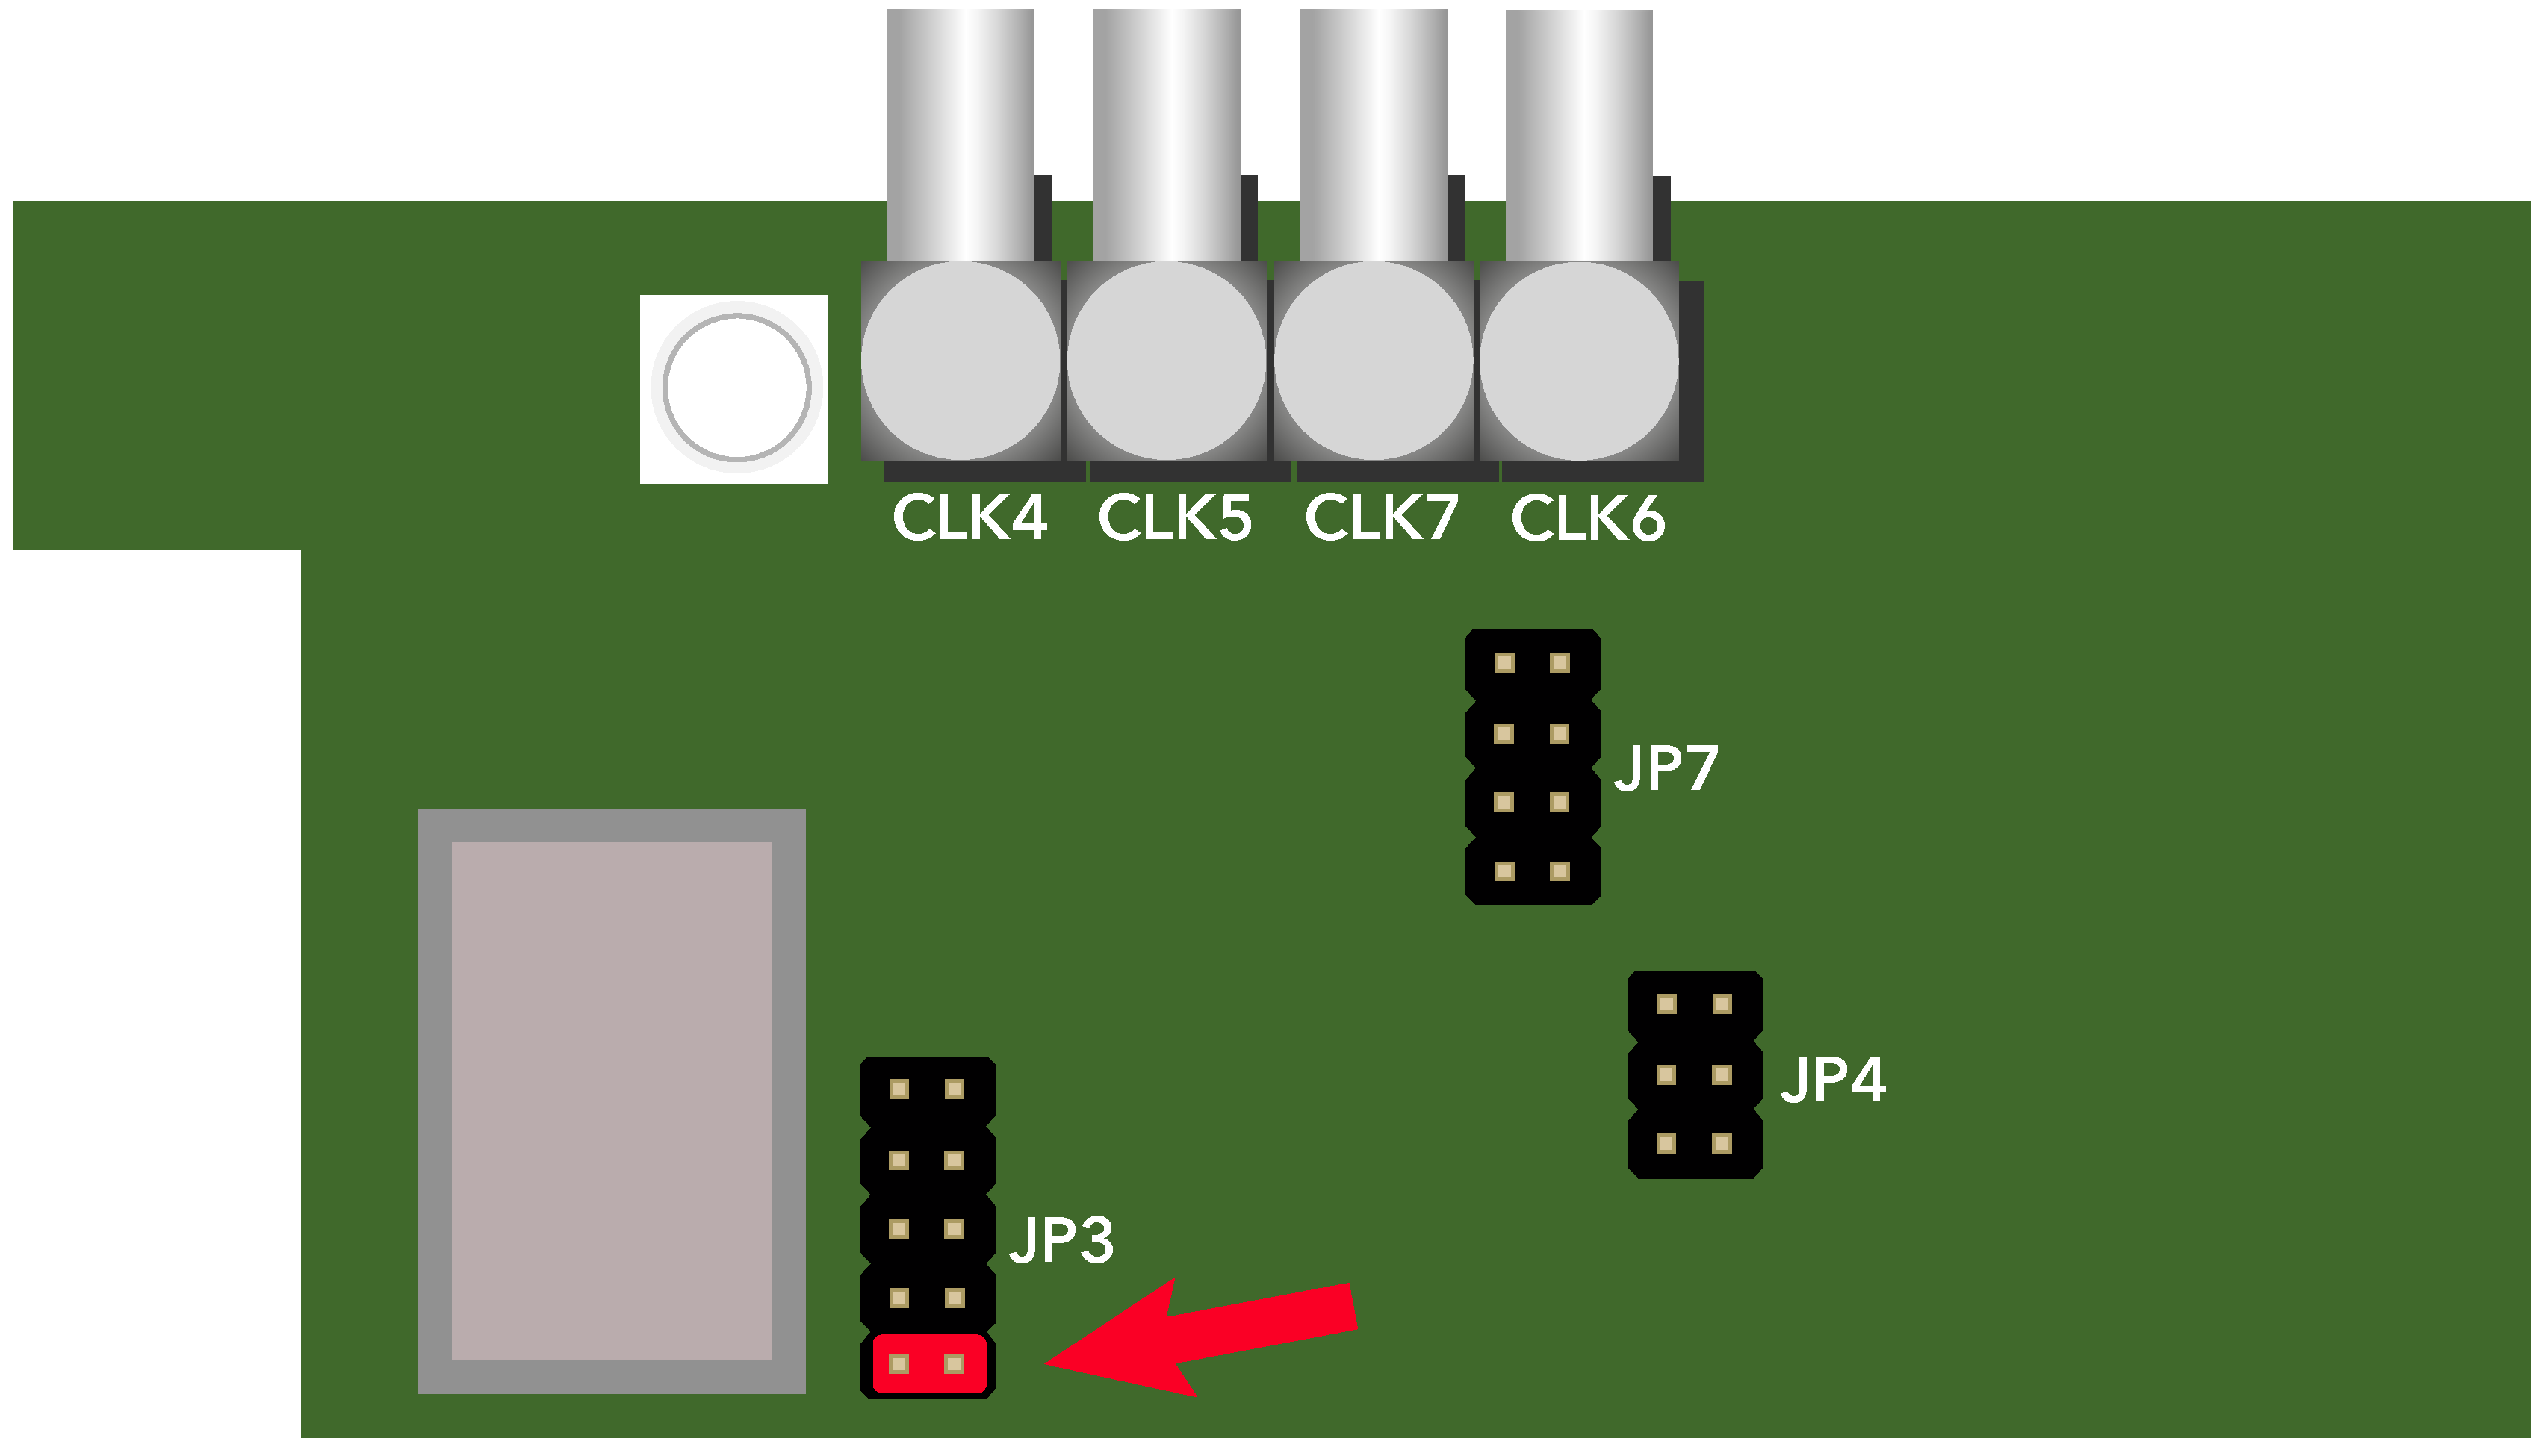
\includegraphics[width=0.5\textwidth]{xhptdc/figures/clockbox.pdf}				
					\caption{ClockBox jumper setting for 10~MHz.\label{fig:clockbox}}
				\end{center} 
			\end{figure*}
			%
		
		\subsection{Crates for multiple boards}
			Most PC mainboards don't have enough PCIe slots to support eight \deviceName s. 
			We offer external enclosure called "Ndigo Crate" that PCIe-over-cable technology to extend the number of available slots in a system.
			The extension is fully transparent to the host system. There are no additional drivers require. 
			Please see the \href{https://www.cronologic.de/products/pcie/pcie-crates}{product page} at our website \url{www.cronologic.de}.  
		

	

}{}




	




	\chapter{\deviceName\ Functionality}
		\txh{ %TimeTagger Version
The \deviceName\ is a ``classic'' common start time-to-digital converter. 

It records the time difference between a leading or trailing edge on the start input to the leading and trailing edges of the stop inputs. 
Rising and falling edges of the stop channel A-D can be enabled individually. 
The measurements are quantized to $500$~ps for -2G devices and tp $1000$~ps for -1G devices. 
The timestamps are recorded in integer multiples of a bin size of $500$~ps for both board types to simplifiy setups where data from differnt board types is combined.
Transitions of the input signals are called hits. To reliably detect hits the signal has to be stable for more than one quantisation interval before and after the edge.  
Triggers on the start channel must not occur less than 5ns apart. The \deviceName\ records events without dead time at a readout rate of about 48MHits/s.
} { %xTDC4 Version
The \deviceName\ is a ``classic'' common start time-to-digital converter. 

It records the time difference between leading or trailing edges on the start input and the stop inputs. 
Each stop channel A-D can be enabled individually. 
The standard deviation of the timestamps is approx. $8$~ps. 
The timestamps are recorded in integer multiples of a bin size of $5/(3\cdot 128) = 13.0208\overline{3}$~ps. 
The data acquisition can be limited to rising or falling signal transitions. 

The maximum trigger rate on the start channel is 4~MHz.

\subsection{Handling of Difficult Hits}
    \label{difficulthits}
    Transitions of the input signals are called hits. To measure all hits with the maximum resolution the hits must fulfill all criteria set forth in this document.
    However, the \deviceName does include mechanisms to provide as much information as possible for hits that fall out of these specs.

    To reliably detect hits the signal has to be stable for at least $900$~ps before and after the edge that is to be measured. 
    Pulses as short as $250$~ps are usually detected at full resolution but have a significant chance to be assigned to the wrong group or appear out of order. 
    For these hits bit 7 in the data word is set. See section \ref{flags} for more information on the data format.

    Between multiple hits on a stop channel a deadtime of approximately $5$~ns is required for full resolution. 
    Hits that are closer together will only be reported with a resolution of $5/6~ns = 833,\overline{3}~ps$. For these hits both bits 6 and 7 are set.

    Data is copied from the 15-entry L0 FIFO to the larger downstream FIFOs at a reate of about $12$~MHz per channel. 
    If the L0 FIFO overflows the hig resolution measurement of some hits will be discarded. 
    In this case a measurement from an alternative TDC wil be used that has a resolution of about $150$~ps. 
    For these hits bit 6 in the data word will be set
} { %xHPTDC8 version
    The \deviceName\ is a streaming time-to-digital converter. It records the timestamps of changes at the inputs A-H in an infinite stream. 
    A flexible grouping mode is available that can emulate common-start or common-stop behaviour. See section \ref{grouping} for details.

    For each channel it can be selected individually whether rising or falling edges are recorded. It is not possible to record both edges of the same channel. 
    The timestamps are recorded in integer multiples of a bin size of $5/(3\cdot 128) = 13.0208\overline{3}$~ps. 
    There must be at least 5~ns between consecutive hits on the same input channel to be detected reliably. 
    The \deviceName\ records events without dead time at a readout rate of about 48MHits/s.
} 
		\section{Grouping and Events}
\label{grouping}
\ifxHPTDC{
    If \textsf{config.tdc\tu mode} is set to \textsf{\PREFIX TDC\tu MODE\tu GROUPING} the TDC will operate in grouping mode. 
    In grouping mode each call to \textsf{xhptdc8\tu read\tu hits()} will return a group of timestamps relative to some trigger event. 
    Otherwise the call returns all available timestamps as absolute timestamps counting upwards from \textsf{xhptdc8\tu start\tu capture()}
}{} 

In typical applications a start hit is followed by a multitude of hits on e.g. a detector. 
The hits recorded are managed in groups (which are called ``events'' in some applications). 
%
\begin{figure*}[ht]
    \begin{center}
        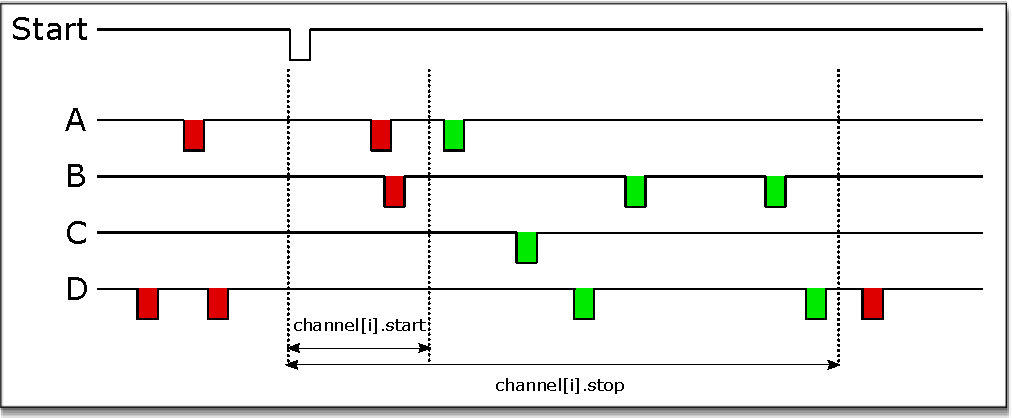
\includegraphics[width=0.7\textwidth]{figures/grouping.pdf}
        \caption{Acquired hits are merged to groups as explained in the text.\label{fig:grouping}}
    \end{center}
\end{figure*}
%

Figure \ref{fig:grouping} shows a corresponding timing diagram. The user can define the range of a group, i.e. the time window within which hits 
on the stop channels are recorded, in software. Hits occurring outside of that time window are discarded. 
 Different ranges can be set for each of the 4 stop channels by setting corresponding values for \textsf{config.grouping.start} and \textsf{.stop} values.

 \ifxHPTDC{
     The values are configured in picoseconds. Negative values can be used in common stop applications.
     \[ -2^{31} <= start <= stop <= 2^{31}-1 \]
 }{
    The values need to be set as multiples of the bin size and must not be negative.
    \[ 0 <= start <= stop <= 2^{16}-1 \]
 }

 In single board setups it is recommended to also configure the gating blocks accordingly. 
 This prevents data from beeing read out that is discarded by the grouping code anyway. 
 Plase note that the grouping parameters are given in picoseconds while the gating blocks are configured in cycles of the 150~MHz clock.


		\lstset{
	language=[Visual]C++,
	keywordstyle=\bfseries\sffamily\color[rgb]{0,0,1},
	identifierstyle=\sffamily,
	commentstyle=\color[rgb]{0.133,0.545,0.133},
	stringstyle=\sffamily\color[rgb]{0.627,0.126,0.941},
	showstringspaces=false,
	basicstyle=\small,
	numberstyle=\footnotesize,
	numbers=left,
	stepnumber=1,
	numbersep=10pt,
	tabsize=2,
	breaklines=true,
	prebreak = \raisebox{0ex}[0ex][0ex]{\ensuremath{\hookleftarrow}},
	breakatwhitespace=false,
	aboveskip={1.5\baselineskip},
	columns=fixed,
	upquote=true,
	extendedchars=true,
}

\section{Auto Triggering Function Generator\label{cp:AutoTriggeringFunctionGenerator}}
Some applications require internal periodic or random triggering. The \deviceName\ function generator provides this functionality.\par

The delay between two trigger pulses of this trigger generator is the sum of two components: A fixed value M and a pseudo random value given by the exponent N. \par

The period is

\begin{align}
    T = 1 + M + [1...2^N]
\end{align}

clock cycles \ifxHPTDC{of the 150~MHz clock}{with a duration of $4~ns$ per cycle}.\par

The trigger can be used as a source for the TiGer unit (see Section \ref{cp:tiger}).


\section{Timing Generator (TiGer)\label{cp:tiger}}
Each digital LEMO-00 input can be used as a \ifxHPTDC{AC coupled}{LVCMOS} trigger output. 
The TiGer function can be configured independently for each connector. 
See Section \ref{cp:tigerblock} for a full description of the configuration options.
% 
\begin{figure*}[ht]
    \begin{center}
        \ifxHPTDC { 
            % this is an XCIrcuit drawing  convertex from postscript with 
            %ps2pdf.exe -dEPSCrop xhptdc8_trigger_matrix.ps
            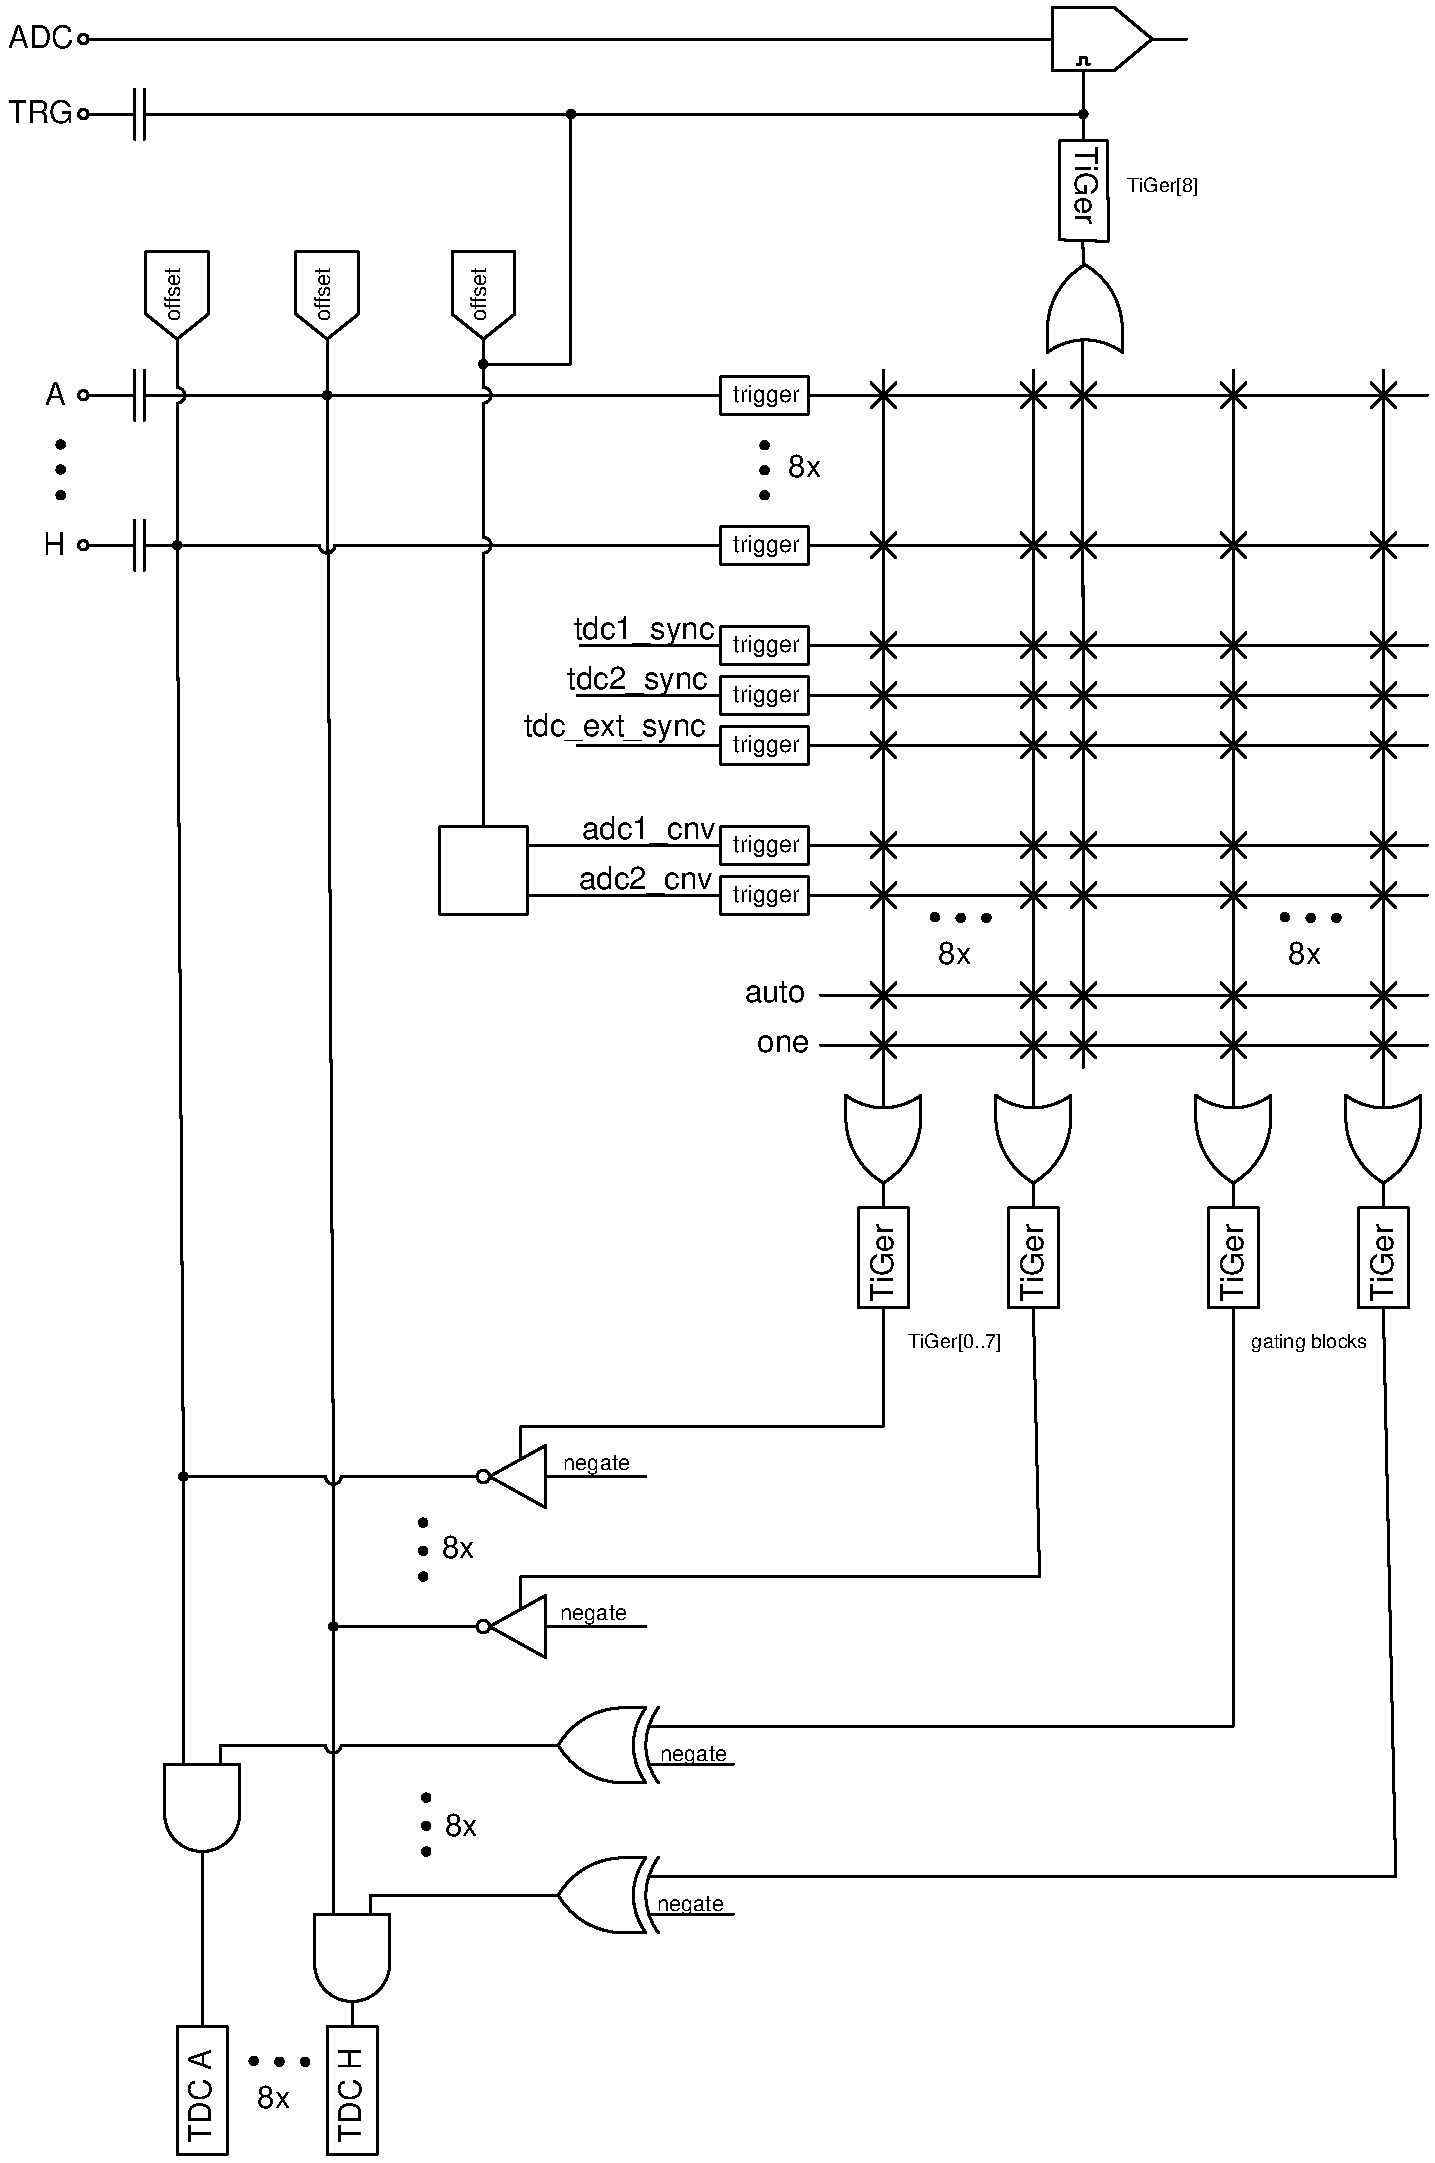
\includegraphics[width=0.6\textwidth]{xhptdc/figures/xhptdc8_trigger_matrix.pdf}
        }{
            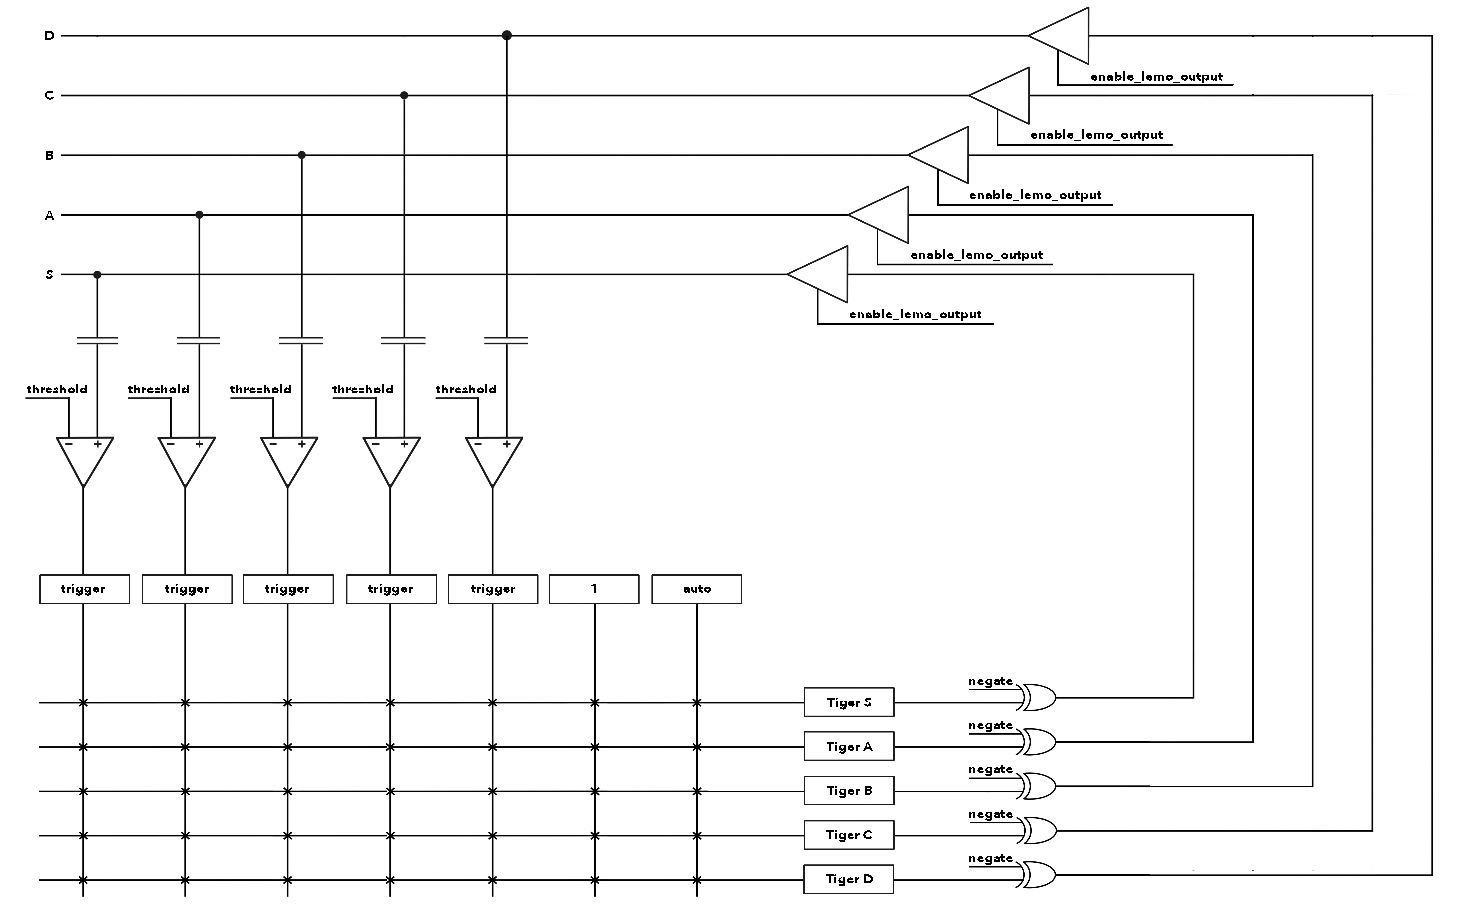
\includegraphics[width=0.7\textwidth]{figures/xTDC4_tiger_matrix.pdf}
        }
        \caption{TiGer blocks can generate outputs that are also available on inputs.\label{fig:matrix}} 
    \end{center}
\end{figure*}
%

Figure \ref{fig:matrix} shows how the TiGer blocks are connected. They can be triggered by an OR of an arbitrary combination of inputs, 
including the auto trigger. Each TiGer can drive its output to its corresponding LEMO connector. This turns the connector into an output. 

When there is an ADC trigger pulse on the TRG connector, either of the two on board ADCs is triggered in an unpredictable pattern. 
If the TRG input shall be used as a trigger the trigger sources must be contain both \textsf{ADC1\tu CNV} and \textsf{ADC21\tu CNV}.

The trigger sources with names ending in \textsf{\tu sync} are managed by the driver for multi board setups and must be left unchanged by the user.

\ifxHPTDC{
	The TiGer outputs are AC coupled to the connector. They can be operated in one of the following modes:
	\paragraph*{\textsf{\PREFIX TIGER\tu OFF}} 
		No signal is output to the connetor. 
	\paragraph*{\textsf{\PREFIX TIGER\tu OUTPUT}} 
		In this mode the connector is input only. Pulses are unipolar with 2V amplitude. 
		Connected hardware must not drive any signals to connectors used as outputs, as doing so could damage both the \deviceName and the external hardware. 
		We recommend to only use short pulses to avoid undesirable baseline shift due to the AC coupling, but the device does not pose any restrictions on the duty cycle. 
		This mode can be used as a clock output with a frequency of $75/N$~MHz for integer $N$.
	\paragraph*{\textsf{\PREFIX TIGER\tu BIDI}} 
		In this mode the TiGer creates unipolar pulses with 1~V amplitude. The connector can still be used as an input. 
		Use short pulses to keep the propability of collision and the effect on the baseline low.	
	\paragraph*{\textsf{\PREFIX TIGER\tu BIPOLAR}} 
		In this mode the connector creates bipolar pulses with 1~V amplitude. The connector can still be used as an input. 
		The pulses have no effect on the baseline offset. 
		TiGer should be configured with $stop = start$ for minimum width bipolar pulses of $2 \times 6.\overline{6}~ns$. 
		The maximum bipolar pulse width is \textsf{XHPTDC8\tu TIGER\tu MAX\tu BIPOLAR\tu PULSE\tu LENGTH = 15}.    
}{
	The TiGer is DC coupled to the connector. Connected hardware must not drive any signals to connectors used as outputs, 
	as doing so could damage both the \deviceName\  and the external hardware.
	Pulses that are short enough for the input AC coupling are available as input signals to the \deviceName. 
	This can be used to measure exact time differences between the generated output signals and input signals on other channels.
}
\ttinput{Tiger_Example.tex}	

\ifxHPTDC{
	\subsection{Triggering the ADC with the TiGer}
		\label{adctiger}
		There is a ninth TiGer that is connected to the trigger input of the ADC. See section \ref{adc} for additional information on the ADC. 

		The ADC TiGer can be used with retrigger enabled to periodically sample ADC data. 
		The period should be no shorter than 300~ns or 45 TiGer clocks.

		The ADC TiGer can also be used to sample voltages at a time relative to one of the TDC inputs. In this case 
		stop should be set to at least 45 to ensure that the sample period criterion is met even when pulses
		arrive in quick succession. A typical application would be to sample some slow control voltage once per start signal.

	\section{Gating}
		Each TDC channel has a second TiGer block that functions as a gate as shown in figure \ref{fig:matrix}. 
		While that output of that gating block is active no hits are recorded in that channel.
		If the block is negated hits are only recorded while the gating block is active.
		
		This is a useful feature in setups where the trigger creates a lot of noise.
		A suitable configuration of the gating block can reduce the bandwidth and buffer usage significantly.
		Gating is performed before the L0 buffer. Grouping is performed in software after readout. 
		
	\section{Triggerable ADC}
		\label{adc}
		The \deviceName\ is equipped with a triggerable ADC. 
		Whenever there is a rising edge on the ADC trigger connector, 
		the voltage on the ADC input connector is sampled. 
		The result is inserted as a packet with timestamp and ADC value into the readout data stream.

		The ADC trigger also is connected to the output of a TiGer block. 
		This can be used to to trigger the ADC periodical or relative to one of the TDC input as described in section \ref{adctiger}

		The ADC triggers should not be closer than 300ns apart.

		There are two interleaved ADCs  to ensure that there is always an ADC available even during readout. 
		This is exposed to the user both in the output data format and in the TiGer and Gating trigger sources.
		When using the ADC trigger as a trigger for Gating or TiGer both trigger sources shall be set to the same value.
		During readout the user shall not distinguish between data from the two ADCs unless advanced calibration is 
		desired for the ADC data. In that case the two ADCs should be treated separately.   

}{} 

	\chapter{Driver Programming API\label{cp:api}} 
		% also includes common/StructConfig.tex and common/InfoStructs.tex
		\ifxHPTDC{
	\newcommand{\device}{\cronvar{\prefix manager}{*xhptdc8\tu mgr}}
	\newcommand{\deviceindex}{\device, \cronvar{int}{index}}
	\newcommand{\deviceconfig}{\device}
	\newcommand{\initparameters}{xhptdc8manager\tu init\tu parameters}
}{
	\newcommand{\device}{\cronvar{\prefix device}{*device}}
	\newcommand{\deviceindex}{\device}
	\newcommand{\deviceconfig}{\deviceindex}
	\newcommand{\initparameters}{\prefix init\tu parameters}
}

The API is a DLL with C linkage.\par

The functions provided by the DLL are declared in \textsf{\txh{TimeTagger4}{xTDC4}{xHPTDC8}\tu interface.h}.

\section{Constants}
\ifxHPTDC{
	\crondef{XHPTDC8MANAGER\tu DEVICES\tu MAX 8}\\
	The maximum number of boards supported by the device manager.

	\ttdef{TDC\tu CHANNEL\tu COUNT 8}\\
	The number of TDC input channels.\par

	\ttdef{GATE\tu COUNT 8}\\
	The number of gating blocks. One for each TDC input.\par

	 \ttdef{TIGER\tu COUNT 9}\\
	The number of timing generators. One for each TDC input and one for the adc trigger.\par

	 \ttdef{TRIGGER\tu COUNT 16}\\
	The number of potential trigger sources for the timing generators. One for each TDC input 
	\ifxHPTDC{}{, one for the Start input} plus some specials. 
	 See Section~\ref{cp:tigerblock} for details.\par

}{ 
	\ttdef{CHANNEL\tu COUNT 4}\\
	The number of TDC input channels.\par

	 \ttdef{TIGER\tu COUNT 5}\\
	The number of timing generators. One for each TDC input and one for the start input.\par

	 \ttdef{TRIGGER\tu COUNT 16}\\
	The number of potential trigger sources for the timing generators. One for each TDC input, one for the Start input plus some specials. 
	 See Section~\ref{cp:tigerblock} for details.\par
}


\section{Driver Information}

	Even if there is no board present the driver revision can be queried using these functions.

	\ttvar{int}{get\tu driver\tu revision()}\\
	Returns the driver version, same format as \textsf{\prefix static\tu info.driver\tu revision}. 
	This function does not require a \deviceName\ board to be present.

	\ttvar{const char*}{get\tu driver\tu revision\tu str()}\\
	Returns the driver version including SVN build revision as a string. 

	\ttvar{int}{count\tu devices(}\cronvar{int}{*error\tu code}, \cronvar{char}{**error\tu message)}\\
	\label{countdevices}
	Returns the number of boards present in the system that are supported by this driver.\par


\section {Initialization}

		\ttvar{int}{close(}\device )\\
		Finalizes the driver for this device.

		\ttvar{int}{get\tu default\tu init\tu parameters(}\cronvar{\initparameters}{ *init)}\\
		Sets up the standard parameters. Gets a set of default parameters for \textsf{\prefix init()}. This must always be used to initialize the \textsf{\prefix init\tu parameter()} structure.\par

		\cronvar{\prefix \ifxHPTDC{manager}{device} *}{\prefix init(}\cronvar{\initparameters}{*params}, \\ 
		\cronvar{int}{*error\tu code}, \cronvar{char}{**error\tu message)}\\
		Opens and initializes the \deviceName\ board with the given index. 
		The user must provide pointers to memory locations where the driver can store return values.\\
		\textsf{error\tu code} shall point to an integer for the error code. \\
		\textsf{error\tu message} must point to a pointer to char. The driver will allocate a buffer for zero terminated error messages and store the address of the buffer in the location provided by the user.\par

		The paramter \textsf{params} is a structure of type \textsf{\prefix init\tu parameters} that must be completely initialized.\par

%%%%%%%%%%%%%%%%% struct init_parameters

		\subsection{Structure \initparameters}
			\cronvar{int}{version}\\
			The version number. Must be set to \textsf{\PREFIX API\tu VERSION}.\par

			\ifxHPTDC{}{
				\cronvar{int}{card\tu index}\\
				The index in the list of \deviceName\ boards that should be initialized.\\
				There might be multiple boards in the system that are handled by this driver as reported by \textsf{\prefix count\tu devices}. This index selects one of them. Boards are enumerated depending on the PCIe slot. 
				The lower the bus number and the lower the slot number the lower the card index.\par

				\cronvar{int}{board\tu id}\\
				the global index in all cronologic devices.\\
				This 8 bit number is filled into each packet created by the board and is useful if data streams of multiple boards will be merged. If only \deviceName\ cards are used this number can be set to the \textsf{card\tu index}. 
				If boards of different types that use a compatible data format are used in a system each board should get a unique id.
				Can be changed with \textsf{int \prefix set\tu board\tu id\allowbreak(\prefix device *device, int board\tu id)}.\par
			}

			\cronvar{\tu \tu int64}{buffer\tu size\ifxHPTDC{}{[8]}}\\
			The minimum size of the DMA buffer.\\
			If set to 0 the default size of 16~MByte is used. 
			\ifxHPTDC{}{For the \deviceName\ only the first entry is used.}\par

			\ifxHPTDC{}{
				\cronvar{int}{buffer\tu type}\\
				The type of buffer. Must be set to 0.
				\begin{description}
					\item[]  \ttdef{BUFFER\tu ALLOCATE   0}
					\item[]  \ttdef{BUFFER\tu USE\tu PHYSICAL   1}  // unsupported
				\end{description}
			

				\cronvar{\tu \tu int64}{buffer\tu address}\\
				This is set by \prefix init() to the start address of the reserved memory.\\ 
				The buffers will be allocated with the sizes given above. Make sure that the memory is large enough.\par
			}

			\cronvar{int}{variant}\\
			Set to 0. Can be used to activate future device variants such as different base frequencies.\par

			\cronvar{int}{device\tu type}\\
			A constant for the different devices of cronologic \textsf{CRONO\tu DEVICE\tu *}.\\
			Initialized by \textsf{\prefix get\tu default\tu init\tu parameters()}. This value is identical to the PCI Device ID. Must be left unchanged.

			\begin{tabular}{ll}
				\crondef{CRONO\tu DEVICE\tu HPTDC}       & 0x1 \\
				\crondef{CRONO\tu DEVICE\tu NDIGO5G}     & 0x2 \\
				\crondef{CRONO\tu DEVICE\tu NDIGO250M}   & 0x4 \\
				\crondef{CRONO\tu DEVICE\tu xTDC4}       & 0x6 \\
				\crondef{CRONO\tu DEVICE\tu TIMETAGGER4} & 0x8 \\
				\crondef{CRONO\tu DEVICE\tu XHPTDC8}     & 0xC \\
				\crondef{CRONO\tu DEVICE\tu NDIGO6}      & 0xD \\
			\end{tabular}

			\cronvar{int}{dma\tu read\tu delay}\\
			The update delay of the write pointer after a packet has been sent over PCIe. Specified in multiples of 16~ns.
			Should not be changed by the user.\par

			\ifxHPTDC{
				\cronvar{int}{multiboard}\\
				Set if multiple devices shall be synchronized.\par
	
				\cronvar{int}{use\tu ext\tu clock}\\
				If set to 1 use external 10 MHz reference. If set to 0 use internal reference.\par

				\cronvar{int}{ignore\tu calibration}\\
				Leave at 0 to use device calibration data.\par
		
			}{
				\cronvar{int}{use\tu ext\tu clock}\\
				If set to 1 use external 10 MHz reference. If set to 0 use internal reference.\par	
			}
	

	
	% info structures
	\input{common/InfoStructs.tex}

	

	\section{Configuration}
		\ifxHPTDC{
			All \deviceName\ boards in the system are configured by a single configuration structure which in turn contains sub structures that configure the individual boards.
		}{
			The device is configured with a configuration structure. 
		}
		The user should first obtain a structure that contains the default settings of the device read from an on-board ROM, 
		then modify the structure as needed for the user application and use the result to configure the device.\par


		\ttvar{int}{configure(}\deviceconfig, \\ \cronvar{\prefix \ifxHPTDC{manager\tu }{}configuration}{*config)}\\
		Configures the \deviceName\ manager.\par

		\ttvar{int}{get\tu current\tu configuration(}\deviceconfig, \\ \cronvar{\prefix \ifxHPTDC{manager\tu }{}configuration}{*config)}\\
		Gets current configuration. Copies the current configuration to the specified config pointer.\par

		\ttvar{int}{get\tu default\tu configuration(}\deviceconfig, \\ \cronvar{\prefix \ifxHPTDC{manager\tu }{}configuration}{*config)}\\
		Gets default configuration. Copies the default configuration to the specified config pointer.\par


	%%%%%%%%%%%%%%%%% configuration structure mostly shared between devices
	\input{common/StructConfig.tex}



	
  
		  
	\chapter{Run Time Control\label{cp:readout}}  % and packet format
		\ifxHPTDC{
				%%%%%%%%%%%%%%%%% run time control
	\section{Controlling the State of the Driver}
	Once the devices are configured the following functions can be used to control the behaviour of the devices. 
	All of these functions return quickly with very little overhead, but they are not guaranteed to be thread safe.

		\ttvar{int}{start\tu capture(}\device)\\
		Start data acquisition.\par

		\ttvar{int}{pause\tu capture(}\device)\\
		Pause a started data acquisition. 
		Pause and continue have less overhead than start and stop but don't allow for a configuration change.\par

		\ttvar{int}{continue\tu capture(}\device)\\
		Call this to resume data acquisition after a call to \textsf{\prefix pause\tu capture()}.
		Pause and continue have less overhead than start and stop but don't allow for a configuration change.\par

		\ttvar{int}{stop\tu capture(}\device)\\
		Stop data acquisition.\par

		\ttvar{int}{start\tu tiger(}\device, \cronvar{int}{index})\\
		\ttvar{int}{stop\tu tiger(}\device, \cronvar{int}{index})\\
		Start and stop the timing generator of an individual board. 
		This can be done independently of the state of the data acquisition.\par	


\section{Readout}

\ttvar{int}{read\tu hits(}\device,  \cronvar{TDCHit}{*hit\tu buf,} \cronvar{size\tu t}{size} )\\
Read a multitude of hits into a buffer provided by the user. Returns the number of read hits.\\
If grouping is enabled a single group is read. 
If the group is to large for the buffer the remaining hits of the group are discarded.\\*
If grouping is disabled, all availabe data is read up to the size of the buffer. \\
The method always returns immediately. If no hits are read it of is beneficial to call \textsf{sleep()} 
or yield the CPU to another process instead of trying again immediately.\\
Make sure to set \textsf{size} to the number of elemenst that fit into the buffer.\\*

This function is not thread safe. 
If you want to process the read data in multiple threads the data needs to be copied to a seperate buffer for each thread.






		}{
			% NOTE: xHPTDC has a seperate file describing the readout

%%%%%%%%%%%%%%%%% run time control
\section{Run Time Control}
	\ttvar{int}{start\tu capture(}\device)\\
	Start data acquisition.\par

	\ttvar{int}{pause\tu capture(}\device)\\
	Pause a started data acquisition. 
	Pause and continue have less overhead than start and stop but don't allow for a configuration change.\par

	\ttvar{int}{continue\tu capture(}\device)\\
	Call this to resume data acquisition after a call to \textsf{\prefix pause\tu capture()}.
	Pause and continue have less overhead than start and stop but don't allow for a configuration change.\par

	\ttvar{int}{stop\tu capture(}\device)\\
	Stop data acquisition.\par

	\ttvar{int}{start\tu tiger(}\device)\\
	Start timing generator. This can be done independently of the state of the data acquisition.\par

	\ttvar{int}{stop\tu tiger(}\device)\\
	Stop timing generator. This can be done independently of the state of the data acquisition.\par

%%%%%% readout
\section{Readout}
	\ttvar{int}{acknowledge(}\device, \cronvar{crono\tu packet}{*packet)}\\
	Acknowledges the processing of the last read block. This is only necessary if \textsf{\prefix read()} is not called with 
	\textsf{in.acknowledge\tu last\tu read} set.\\
	This feature allows to either free up partial DMA space early if there will be no call to \textsf{\prefix read()} anytime soon. 
	It also allows to keep data over multiple calls to \textsf{\prefix read()} to avoid unnecessary copying of data. \par

	\ttvar{int}{read(}\device \cronvar{\prefix read\tu in}{*in,} \\ \cronvar{\prefix read\tu out}{*out)}\\
	Return a pointer to an array of captured data in \textsf{read\tu out}. 
	The result can contain any number of packets of type \textsf{\prefix packet}.
	\textsf{read\tu in} provides parameters to the driver. 
	A call to this method automatically allows the driver to reuse the memory returned in the previous call if \textsf{read\tu in.acknowledge\tu last\tu read} is set.\\
	Returns an error code as defined in the structure \textsf{\prefix read\tu out}.

	\subsection{Input Structure \prefix read\tu in}

		\ttvar{\prefix bool\tu t}{acknowledge\tu last\tu read}\\
		If set \textsf{\prefix read()} automatically acknowledges packets from the last read. 
		Otherwise \textsf{\prefix acknowledge()} needs to be called explicitely be the user. 

	\subsection{Input Structure \prefix read\tu out}
		\cronvar{crono\tu packet}{*first\tu packet}\\
		Pointer to the first packet that was captureed by the call of \textsf{\prefix read()}.\par

		\cronvar{crono\tu packet}{*last\tu packet}\\
		Address of header of the last packet in the buffer.\par

		\cronvar{int}{error\tu code}\\
		Assignments of the error codes.\par
		\begin{tabular}{lc}
			\crondef{CRONO\tu READ\tu OK} & 0\\
			\crondef{CRONO\tu READ\tu NO\tu DATA} & 1\\
			\crondef{CRONO\tu READ\tu INTERNAL\tu ERROR} & 2\\
			\crondef{CRONO\tu READ\tu TIMEOUT} & 3\par
		\end{tabular}\par

		\cronvar{const char}{*error\tu message}
		The last error in human readable form, possibly with additional information on the error.

	
		} 

	\chapter{Output Data Format\label{cp:packetformat}} 
		\ifxHPTDC{
			For each measured edge the \deviceName\ creates a 12 byte data structure TDCHit that contains a 64 bit timestamp in picoseconds and three fields with additional information. 

\section{Structure TDCHit}
\label{TDCHit}
\cronvar{long long}{time}\\
The time stamp of the hit in picoseconds. 

If grouping is disabled the timestamps are continuously counting up from the call to \textsf{start\tu capture()}.

If grouping is enabled the timestamps are relative to the trigger or the separate zero reference of the group. 
The first of a group has channel number 255 and provides the absolute time of the group. 
The absolute time of each of the hits can be obtained by adding this value to each of the relative timestamps.

\cronvar{unsigned char}{channel}\\
For the first board in the system this is 0 to 7 for the TDC channels A to H. 8 or 9 for ADC data. Data from channels 8 and 9 should usually be treated as data from the same channel. 
For the other boards the channel number is incremented by $board\_id \cdot 10$.
In grouping mode the first hit of each group has channel number 255 and contains the absolute time of the group.

\cronvar{unsigned char}{type}\\
Additional information on the type of hit recorded. See section \ref{hittypes}.

\cronvar{unsigned short}{bin}\\
For ADC hits this contains the sampled voltage. For TDC hits the content is undefined.

\newpage
\subsection{TDCHit Types \label{hittypes}}
\newcommand{\HTYPE}{\PREFIX TDCHIT\tu TYPE\tu}

\paragraph*{Type information for TDC measurements}
If the hit is a TDC measurement on channels A to H the following flags are defined for the \textsf{type} field of the TDCHit structure:\\*
\begin{tabular}{lc}
    \crondef{\HTYPE RISING} & 0x01\\
    \indent Rising edge &\\
    \crondef{\HTYPE ERROR}  & 0x02\\
    \indent any type of error& \\
    \crondef{\HTYPE ERROR\tu TIMESTAMP\tu LOST}  & 0x04\\
    \indent Hits missing due to L1 FIFO overflow&\\
    \crondef{\HTYPE ERROR\tu ROLLOVER\tu LOST}  & 0x08\\
    \indent Invalid timestamp due to internal error&\\
    \crondef{\HTYPE ERROR\tu PACKET\tu LOST}  & 0x10\\
    \indent Hits missing due to a lost DMA packet&\\
    \crondef{\HTYPE ERROR\tu SHORTENED}  & 0x20\\
    \indent Hits missing due to a shortened DMA packet&\\
    \crondef{\HTYPE ERROR\tu DMA\tu FIFO\tu FULL}  & 0x40\\
    \indent Hits missing due to L2 FIFO overflow&\\
    \crondef{\HTYPE ERROR\tu HOST\tu BUFFER\tu FULL}  & 0x80\\
    \indent Hits missing due to host buffer overflow &\\
\end{tabular}

If hits are missing the error flag is set on the next hit from the same board that is read out.

\paragraph*{Type information for ADC measurements}
If the hit is an ADC measurement on channels 8 or 9 the following flags are defined for the \textsf{type} field of the TDCHit structure:\\*
\begin{tabular}{lc}
    \crondef{\HTYPE ADC\tu INTERNAL} & 0x01\\
    \indent ADC measurement triggered by TiGer &\\
    \crondef{\HTYPE ADC\tu ERROR}  & 0x02\\
    \indent any type of error& \\
    \crondef{\HTYPE ADC\tu ERROR\tu INVALID\tu TRIGGER}  & 0x08\\
    \indent TRG input violated timing requirements. Data may be corrupted&\\
    \crondef{\HTYPE ADC\tu ERROR\tu DATA\tu LOST}  & 0x10\\
    \indent ADC measurement missing due to overflow of any buffer&\\
\end{tabular}

If hits are missing the error flag is set on the next hit from the same board that is read out.


 
		}{
			


\section{Output Structure crono\tu packet}

	\cronvar{unsigned char}{channel}\\
	Unused, always 0.\par

	\cronvar{unsigned char}{card}\\
	Identifies the source card in case there are multiple boards present. Defaults to 0 if no value is assigned to the parameter \textsf{board\tu id} in Structure \textsf{ndigo\tu init\tu parameters}.\par

	\cronvar{unsigned char}{type}\\
	The data stream consists of 32-bit unsigned data as signified by a value of 6.\par

	\cronvar{unsigned char}{flags}\\
	\indent\ttdef{ PACKET\tu FLAG\tu ODD\tu HITS} 1\\
	\indent The last data word in the data array consists of one timestamp only which is located in the lower 32 bits of the 64-bit data word (little endian).\par
	\indent\ttdef{ PACKET\tu FLAG\tu SLOW\tu SYNC} 2\\
	\indent Start pulse distance is larger than the extended timestamp counter range.\par
	\indent\ttdef{ PACKET\tu FLAG\tu START\tu MISSED} 4\\
	\indent The trigger unit has discarded packets due to a full FIFO.\par
	\indent\ttdef{ PACKET\tu FLAG\tu SHORTENED} 8\\
	\indent The trigger unit has shortened the current packet due to full FIFO.\par
	\indent\ttdef{ PACKET\tu FLAG\tu DMA\tu FIFO\tu FULL} 16\\
	\indent The internal DMA FIFO was full. Might or might not result in dropped packets.\par
	\indent\ttdef{ PACKET\tu FLAG\tu HOST\tu BUFFER\tu FULL} 32\\
	\indent The host buffer was full. Might or might not result in dropped packets.\par

	\cronvar{unsigned int}{length}\\
	Number of 64-bit elements (each containing up to 2 TDC hits) in the data array.\par

	\cronvar{unsigned \tu\tu int64}{timestamp}\\
	Coarse timestamp of the start pulse. Values are given in multiples of \itett{$500$~ps}{$5/3=1.\overline{6}$~ns}.\par

	\cronvar{unsigned \tu\tu int64}{data[1]}\\
	TDC hits. the user can cast the array to uint32* to directly operate on the TDC hits.

	\noindent
	\begin{small}
	\begin{tabular}{|c||p{9cm}|p{1,5cm}|p{1,5cm}|}
		\hline
		bits & 31~ ~ ~ ~ ~ ~ ~ ~ ~ ~ ~ ~ ~ ~ ~ ~ ~ to ~ ~ ~ ~ ~ ~ ~ ~ ~ ~ ~ ~ ~ ~ ~ ~ ~ 8 & 7~ ~ to ~ ~ 4 & 3~ ~ to ~ ~ 0\\\hline
		content & TDC DATA & FLAGS & CHN \\\hline
	\end{tabular}
	\end{small}

	The timestamp of the hit is stored in bits 31 down to 8 in multiples of 
	\itett{500~ps. For the -1G Variant bit 8 is always 0.}{
		$5/(3*128) = 13.0208\overline{3}$~ps
	}\\
	
	\label{flags}
	Bits 7 down to 4 are hit flags:\par
	\itett{
		Bit 7: Always 0.\par
		Bit 6: Always 1.\par
	} {
		Bit 7, 6: Resolution of this measurement. \ifxHPTDC{}{See section \ref{difficulthits}}.\\
		\noindent
		\begin{small}
		\begin{tabular}{|c|c||l|}
			\hline
			bit 7 & bit 6 & Measurement Type \\\hline\hline
			0 & 0 &  Normal full resolution measurement.\\\hline
			0 & 1 &  Measurement performed with carry chain TDC at about 150~ps resolution.\\\hline
			1 & 0 &  Full resolution measurement that might in the wrong place in the data stream.\\\hline
			1 & 1 &  Measurement with only $5/6~ns = 833.\overline{3}~ps$ resolution. \\\hline
		\end{tabular}
		\end{small}
		
	}
	Bit 5: Rollover. The time since start pulse exceeded the \itett{23}{24}-bit range that can be ecnoded in a data word. This word does not encode a measurement. 
	Instead the readout software should increment a rollover counter that can be used as the upper bits of consecutive time stamps.  
	The counters should be reset for each packet.
	The total offset of a hit in picoseconds can be computed by
	\[	\Delta T_{hit} = \mathrm{(\#\ rollovers \cdot 2^{\itett{23}{24}} + TDC\_ DATA_{hit}) \cdot \itett{timetagger4}{xtdc4}\_param\_info.binsize} \]
	\indent
	Bit 4: Set if this word encodes a rising edge. Otherwise, this word belongs to a falling edge.
	The channel number is given in the lowest nibble of the data word. A value of 0 corresponds to channel A, a value of 3 to channel D.\par
 
		}  
 
	\chapter{C Example}  
		% SVN Info:
% $Date: 2021-01-31 20:06:56 +0100 (So, 31 Jan 2021) $
% $Rev: 1040 $
% $Author: kolja $

	The following C++ source code shows how to initializes a \deviceName\ board, configure it and loop over incoming packets.	

	If you are reading this documentation in portable document format, the source code of the C example is also embedded as an
	\txh{
		\textattachfile[color=cronlightgreen, description={Example Source Code}]{"timetagger/example.cpp"}{attachment}
		to the file. You can open it in an external viewer or save it to disk by clicking on it.
		\lstinputlisting{timetagger/example.cpp}
	}{
		\textattachfile[color=cronlightgreen, description={Example Source Code}]{xtdc/example.cpp}{attachment}
		to the file. You can open it in an external viewer or save it to disk by clicking on it.
		\lstinputlisting{xtdc/example.cpp}
	}{	
		\textattachfile[color=cronlightgreen, description={Example Source Code}]{xhptdc/example.cpp}{attachment}
		to the file. You can open it in an external viewer or save it to disk by clicking on it.

		The example code is managed as open source on GitHub at 
		\href{https://github.com/cronologic-de/xhptdc8_babel/tree/main/ug_example}{https://github.com/cronologic-de/xhptdc8\tu babel}. 
		The repository contains a complete project for Microsoft Visual Studio that you can use to compile the example.
		Examples for more programming languages such as Golang, Rust, Python and LabView will be added to the repository over time.

		At the time this document is written, the following source code can be found in the repository:
		\begin{itemize}
			\item \href{https://github.com/cronologic-de/xhptdc8_babel/tree/main/dummy}{dummy library} to be able to develop code for the \deviceName\ without a physical board beeing present
			\item \href{https://github.com/cronologic-de/xhptdc8_babel/tree/main/util}{utility library} to configure the device from YAML strings or YAML files 
			\item command line info tool to list information about all \deviceName\ boards in the system. This tool is written in Go.
		\end{itemize}

		\lstinputlisting{xhptdc/example.cpp}
	}
	% there were problems with underscores in file names so we removed them



	\chapter{Technical Data}    
		\ttinput{Tech.tex} 
		% SVN Info:
% $Date: 2021-01-29 22:28:41 +0100 (Fr, 29 Jan 2021) $
% $Rev: 1039 $
% $Author: kolja $
\section{Electrical Characteristics}

	\subsection{Power Supply}

		\noindent
		\begin{tabularx}{\textwidth}{|c|X|c|c|c|c|}
			\hline
			Symbol & Parameter & Min & Typical & Max & Units\\
			\hline\hline
			P & Total power consumption &&& 25& W\\
			\hline
			I & PCIe 3,3V rail input current &&&4& mA\\
			\hline
			VCC & PCIe 3,3V rail power supply voltage &3,1&3,3&3,5& V\\
			\hline
			I & PCIe 12V rail input current &&&2,1& A\\
			\hline
			VCC & PCIe 12V rail power supply voltage &11,1&12&12,9& V\\
			\hline
			I & PCIe 3,3VAux rail input current &&0&& A\\
			\hline
			VCC & PCIe 3,3VAux rail power supply voltage &&3,3&& V\\
			\hline
		\end{tabularx}

	\subsection{TDC Inputs}

		The \deviceName's inputs are single-ended AC-coupled with 50$\Omega$ DC termination.

		\noindent
		\begin{tabularx}{\textwidth}{|c|X|c|c|c|c|}
			\hline
			Symbol & Parameter & Min & Typical & Max & Units\\
			\hline\hline
			V\subscript{Base} & Input Baseline & 0 & & 5 & V\\
			\hline
			V\subscript{Threshold} & Trigger Level & V\subscript{Base} - 1.32 & & V\subscript{Base} + 1.18 & V\\
			\hline
			t\subscript{Pulse} & Pulse Length & 2 & 5 & 200 & ns\\
			\hline
			t\subscript{Rise} & Pulse Edge 20\% to 80\%  &  &  & 10 & ns\\
			\hline
			t\subscript{Fall} & Pulse Edge 80\% to 20\%  &  &  & 10 & ns\\
			\hline
			Z\subscript{P} & Input Impedance && 50 && $\Omega$\\
			\hline
			I\subscript{Term} & Termination Current & -50 & -20 & 50 & mA\\
			\hline
		\end{tabularx}

	All inputs are AC coupled. The inputs have very high input bandwidth requirements and therefore there are no circuits that provide over voltage protection for these signals. 
	Any voltage on the inputs above 5V or below -5V relative to the voltage of the slot cover can result in permanent damage to the board.
	
	\ifxHPTDC{
		All digital inputs can output AC coupled pulses from the TiGer. 
		Special care should be taken not to enable the TiGer output when sensitive equipment is connected that could be damaged by the pulses. 
	}{
		Make sure not to drive the inputs when the connector is configured as a TiGer output. 
	}
	See Section \ref{cp:tiger}. 
%%%%%%%%%%% ADC input
	\ifxHPTDC{
	\newpage
	\subsection{ADC Inputs}
	The ADC input is DC coupled to a differential termination voltage of 400~mV. 
	This means that the actual voltage seen by the ADC will depend on the output impedance of the source that is driving the input.\\*
	\noindent
		\begin{tabularx}{\textwidth}{|c|X|c|c|c|c|}
			\hline
			Symbol & Parameter & Min & Typical & Max & Units\\
			\hline\hline
			V\subscript{in} & Input voltage & -2.0 &  & 2.5 & V \\
			\hline 
			V\subscript{term} & Termination voltage & & 0.4 & & V \\
			\hline 
			Z\subscript{in} & Input Impedance & & 50  & & $\Omega$ \\
			\hline
		\end{tabularx}

%%%%%%%%%%% clock input		
	\subsection{Clock input J2}
	The ADC input is DC coupled to a differential termination voltage of 400~mV. 
	This means that the actual voltage seen by the ADC will depend on the output impedance of the source that is driving the input.\\*
	\noindent
		\begin{tabularx}{\textwidth}{|c|X|c|c|c|c|}
			\hline
			Symbol & Parameter & Min & Typical & Max & Units\\
			\hline\hline
			V\subscript{p-p} & Peak to Peak voltage & 1 &  & 3.3 & V \\
			\hline 
			V\subscript{cm} & Common mode voltage voltage &-3 & 0 & 3 & V \\
			\hline 
			V\subscript{tck} & Clock termination voltage & & 0 &  & V \\
			\hline 
			Z\subscript{in} & Input Impedance & & 50  & & $\Omega$ \\
			\hline 
			D\subscript{J2} & Duty cycle & 45 & 50 & 55 & \% \\
			 \hline 
			 f\subscript{J2}& Frequency &  & 10 &  & MHz \\
			\hline
		\end{tabularx}
}{}

\newpage
\section{Information Required by DIN EN 61010-1}
\subsection{Manufacturer\label{cp:manu}}

The \deviceName\ is a product of:\

\begin{quote}
	cronologic GmbH \& Co. KG\\
	Jahnstra\ss{}e 49\\
	60318 Frankfurt\par
	Germany
	\noindent HRA 42869 beim Amtsgericht Frankfurt/M\par
	\noindent VAT-ID: DE235184378
	\noindent PCI Vendor ID: 0x1A13
\end{quote}

\subsection{Intended Use and System Integration}

	The devices are not ready to use as delivered by cronologic. It requires the development of specialized software to fulfill the application of the end user. The device is provided to system integrators to be built into measurement systems that are distributed to end users. These systems usually consist of the \deviceName, a main board, a case, application software and possible additional electronics to attach the system to some type of detector. They might also be integrated with the detector.\par

	The \deviceName\ is designed to comply with DIN EN 61326-1 when operated on a PCIe compliant main board housed in a properly shielded enclosure. 
	When operated in a closed standard compliant enclosure the device does not pose any hazards as defined by EN 61010-1.\par

	Radiated emissions, noise immunity and safety highly depend on the quality of the enclosure. 
	It is the responsibility of the system integrator to ensure that the assembled system is compliant to applicable standards of the country that the system is operated in, especially with regards to user safety and electromagnetic interference. \par
	 
	When handling the board, adequate measures must be taken to protect the circuits against electrostatic discharge (ESD). All power supplied to the system must be turned off before installing the board.

	\subsection{Environmental Conditions for Storage}

	The board shall be stored between operation under the following conditions:

	\noindent
	\begin{tabularx}{\textwidth}{|c|X|c|c|c|c|}
		\hline
		Symbol & Parameter & Min & Typical & Max & Units\\
		\hline\hline
		T & ambient temperature & -30 && 60 & $^{\circ}$C\\
		\hline
		RH & relative humidity at 31$^{\circ}$C noncondensing & 10 && 70 & \%\\
		\hline
	\end{tabularx}


\subsection{Environmental Conditions for Operation}

	The board is designed to be operated under the following conditions:

	\noindent
	\begin{tabularx}{\textwidth}{|c|X|c|c|c|c|}
		\hline
		Symbol & Parameter & Min & Typical & Max & Units\\
		\hline\hline
		T & ambient temperature & 5 && 40 & $^{\circ}$C\\
		\hline
		RH & relative humidity at 31$^{\circ}$C & 20 && 75 & \%\\
		\hline
	\end{tabularx}

	WARNING: Do not connect any DC coupled inputs to a channel while the TiGer of that channel is configured as an output (see Section \ref{cp:tiger}).
	Doing so could do permanent damage to the \deviceName\ and the external hardware.

\subsection{Cooling}

	The \deviceName\ in its base configuration has passive cooling that requires a certain amount of air flow. 
	If the case design can't provide enough air flow to the board, a slot cooler like Zalman ZM-SC100 can be placed next to the board. 
	Active cooling is also available as an option for the board.


\subsection{Recycling}

	cronologic is registered with the ``Stiftung Elektro-Altger\"a{}te Register'' as a manufacturer of electronic systems with Registration ID DE 77895909.\par
	The \deviceName\ belongs to category 6, ``Kleine Geräte der Informations- und Telekommunikationstechnik für die ausschließliche Nutzung in anderen als privaten Haushalten''. 
	Devices sold before 2018 belong to category 9, ``\"U{}berwachungs und Kontrollinstrumente f\"u{}r aus\-schlie\ss lich gewerbliche Nutzung''. 
	
	The last owner of a \deviceName\ must recycle it, treat the board in compliance with \S{}11 and \S{}12 of the German ElektroG, or return it to the manufacturer's address listed on page \pageref{cp:manu}.
	

	\chapter{Revision History} 
		\noindent
		User Guide \hyperlink{ugrev}{\ugrev} as of 2020-02-04\\
		\\
		cronologic GmbH \& Co. KG\\
		Jahnstraße 49\\
		60318 Frankfurt am Main\\Germany\\
		\ttinput{FwRev.tex}
		\ifxHPTDC{\section{Driver \& Applications}
\begin{tabularx}{\textwidth}{|c|c|X|}
    \hline
    Revision & Date & Comments\\
    \hline\hline
    \hypertarget{drvrev}{0.x.x} & 2021 & preliminary driver\\
    \hline
 
\end{tabularx}}{\section{Driver \& Applications}
\begin{tabularx}{\textwidth}{|c|c|X|}
    \hline
    Revision & Date & Comments\\
    \hline\hline
    \hypertarget{drvrev}{1.4.1} & 2019-11-11 & x64 32 mode issues fixed\\
    \hline
    {1.4.0} & 2019-06-04 & Improved Windows 10 support\\
    \hline
    {1.3.0} & 2019-01-23 & Added Windows 10 support\\
    \hline
\end{tabularx}} 
		% Also update date and version in User_Guide.tex

\section{User Guide}
\begin{tabularx}{\textwidth}{|c|c|X|}
    \hline
    Revision & Date & Comments \\
    \hline\hline  
    \hypertarget{ugrev}{1.8.1} & 2021-04-09 &
    \makecell[l]{
        Many corrections and updates to the xHPTDC8 API.
    }\\
    \hline 
    {1.8.0} & 2021-03-22 &
    \makecell[l]{
        Added xHPTDC8 User Guide
    }\\
    \hline 
    {1.7.0} & 2021-02-04 & 
    \makecell[l]{
        Combined User Guide for -1G and -2G \\
        Added characteristics for INL, DNL and Time Base \\
        Reordered sections for clarity \\
        Error corrections for rollovers, binsize and range \\
        Added figure \ref{fig:matrix} (TiGer matrix) \\
        Corrected board revision \\
    }\\
    \hline
    \itett{1.3.0}{1.6.0} & 2019-06-05 & API clarifications \\
    \hline
\end{tabularx} 
\end{document}  "

% or define it here
%\newcommand{\deviceName}{TimeTagger4}
%\newcommand{\deviceName}{xTDC4}

  
\ifthenelse{\isundefined{\deviceName}}{ 
	\message {\\ WARNING: Undefined device name, TimeTagger4 used}
	\newcommand{\deviceName}{TimeTagger4}}{}
\message{\\Device name is \deviceName }


%output the first option for the TimeTagger, the second one otherwise
% example: 
% \itett{THIS IS A TimeTagger4}{THIS IS NOT}
\ifthenelse{\equal{\deviceName}{TimeTagger4}}{\newcommand{\itett}[2]{#1}}{\newcommand{\itett}[2]{#2}}
\itett{\message{\\TIMETAGGER\\}}{\message{\\NO TIMETAGGER\\}}

% output code only for the xHPTDC8 
% example: 
% \ifXHPTDC{THIS IS AN xHPTDC8} {THIS IS NOT}
% NOTE: Macro names may not contain digits
\ifthenelse{\equal{\deviceName}{xHPTDC8}} {\newcommand{\ifxHPTDC}[2]{#1}}{\newcommand{\ifxHPTDC}[2]{#2}}
\ifxHPTDC{\message{\\XHPTDC8\\}}{\message{\\NO XHPTDC\\}}
 
  
 
% output code for the TimeTagger4, xTDC4 or xHPTDC8
% example: 
% \txh{THIS IS A TimeTagger4}{THIS IS AN xTDC4}{THIS IS AN xHPTDC8}
\itett{\newcommand{\txh}[3]{#1}}{\ifxHPTDC{\newcommand{\txh}[3]{#3}} {\newcommand{\txh}[3]{#2}}}
 
\txh{ % TimeTagger4
	\message{Generating User Guide for TimeTagger4}
	\newcommand{\ttinput}[1]{\input{timetagger/#1}}
	\newcommand{\titlefile}{"figures/TT4_title.pdf"}
	\newcommand{\prefix}{timetagger4\tu}
	\newcommand{\PREFIX}{TIMETAGGER4\tu}
}{ % xTDC4
	\message{Generating User Guide for xTDC4}
	\newcommand{\ttinput}[1]{\input{xtdc/#1}}
	\newcommand{\titlefile}{"figures/xTDC4_title.pdf"}
	\newcommand{\prefix}{xtdc4\tu} 
	\newcommand{\PREFIX}{XTDC4\tu}
} 
{ % xHPTDC8
	\message{Generating User Guide for xHPTDC8}
	\newcommand{\ttinput}[1]{\input{xhptdc/#1}}
	\newcommand{\titlefile}{"figures/xHPTDC8_title.pdf"}
	\newcommand{\prefix}{xhptdc8\tu}
	\newcommand{\PREFIX}{XHPTDC8\tu}
} 

\hyphenation{Time-Tagger xTDC xHPTDC cronologic}


\newcommand{\ttvar}[2]{\noindent\textsf{\textbf{\textcolor{crongrey}{#1} \prefix #2}}}%for variable declaration
\newcommand{\ttdef}[1]{\noindent\textsf{\textcolor{crongrey}{\#{}define} \PREFIX #1}}%for definitions

\newcommand{\ugrev}{{1.8.0\tu draft\tu 6}}
%%%%%%%%%%%%%%%%%%%%%%%%%%%%%%%%%
 
\begin{document}  
\cronofront{\titlefile}
 
% 
	\chapter{Introduction}
		\ttinput{Intro.tex}

	\chapter{Hardware}  
		\section{Installing the Board}
The \deviceName\ board can be installed in any PCIe-CEM slot with x1 or more lanes. 
Make sure the PC is powered off and the main power connector is disconnected while installing the board.\par

%
\section{\deviceName\ Inputs and Connectors}
	Figure \ref{fig:bracket} shows the location of the inputs on the slot bracket.
%
	\begin{figure*}[hb]
		\begin{center}
			\ifxHPTDC{
				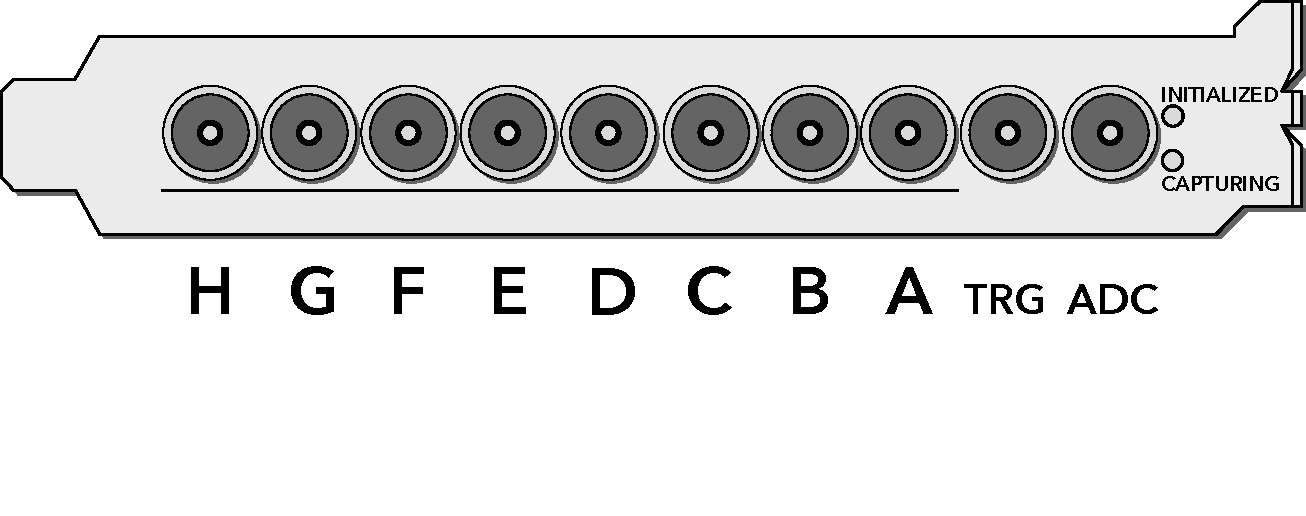
\includegraphics[width=0.6\textwidth]{figures/xHPTDC8_Slotblende.pdf}
			}{
				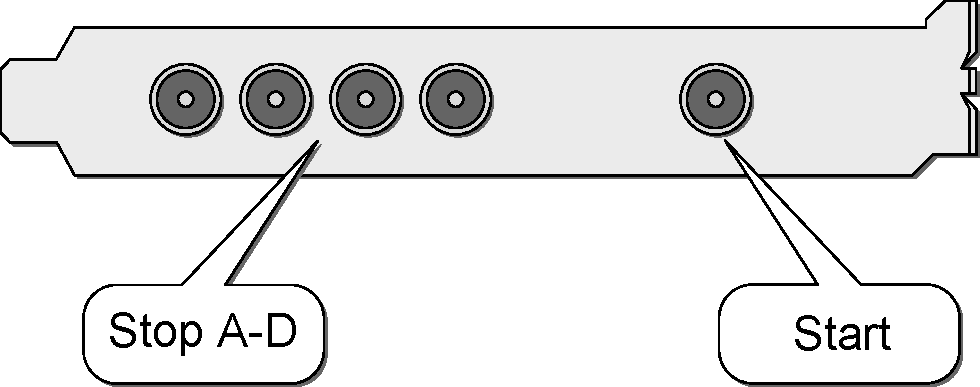
\includegraphics[width=0.6\textwidth]{figures/xTDC4_Slotblende.pdf}
			}
			\caption{Input connectors of the \deviceName\ on the PCIe bracket.\label{fig:bracket}}
		\end{center}
	\end{figure*}
	%
	\begin{figure*}[hb]
		\begin{center}
			\ifxHPTDC{
				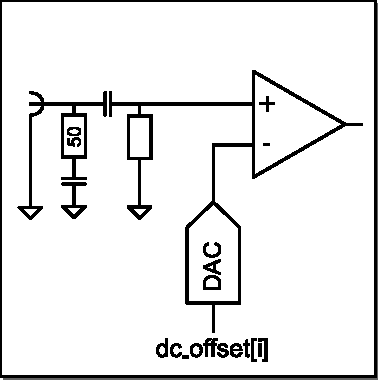
\includegraphics[width=0.3\textwidth]{xhptdc/figures/InputCircuit.pdf}
			}{
				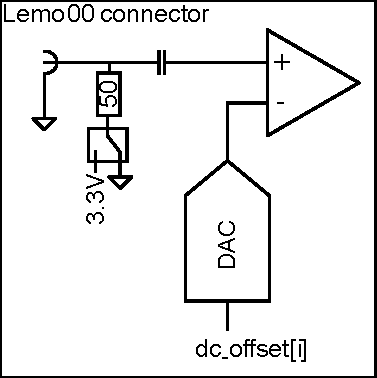
\includegraphics[width=0.3\textwidth]{figures/InputCircuit.pdf}
			}
			\caption{Input circuit for each of the input channels.\label{fig:inputcirc}}
		\end{center}
	\end{figure*}
	%

	Lemo-00 connectors are used for input connection. The inputs are AC-coupled and have an impedance of 50$\Omega$. 
	A schematic of the input circuit is shown in Figure \ref{fig:inputcirc}. 
	The digital threshold for any input can be adjusted to comply with a multitude of single ended signaling standards.
	The threshold can also be used to configure the input for either positive or negative pulses.
	
	
	The connectors can also be used as outputs. 
	\ifxHPTDC{AC-coupled}{DC-coupled} output pulses for automatic internal triggering and control of external devices 
	can be generated using the TiGer timing pattern generator. See section \ref{cp:tiger} for details on TiGer. 
	%
		\begin{figure*}[ht]
			\begin{center}
				\ifxHPTDC{
					\includegraphics[width=0.7\textwidth]{xhptdc/figures/xHPTDC8_schematic.pdf}
				}{
					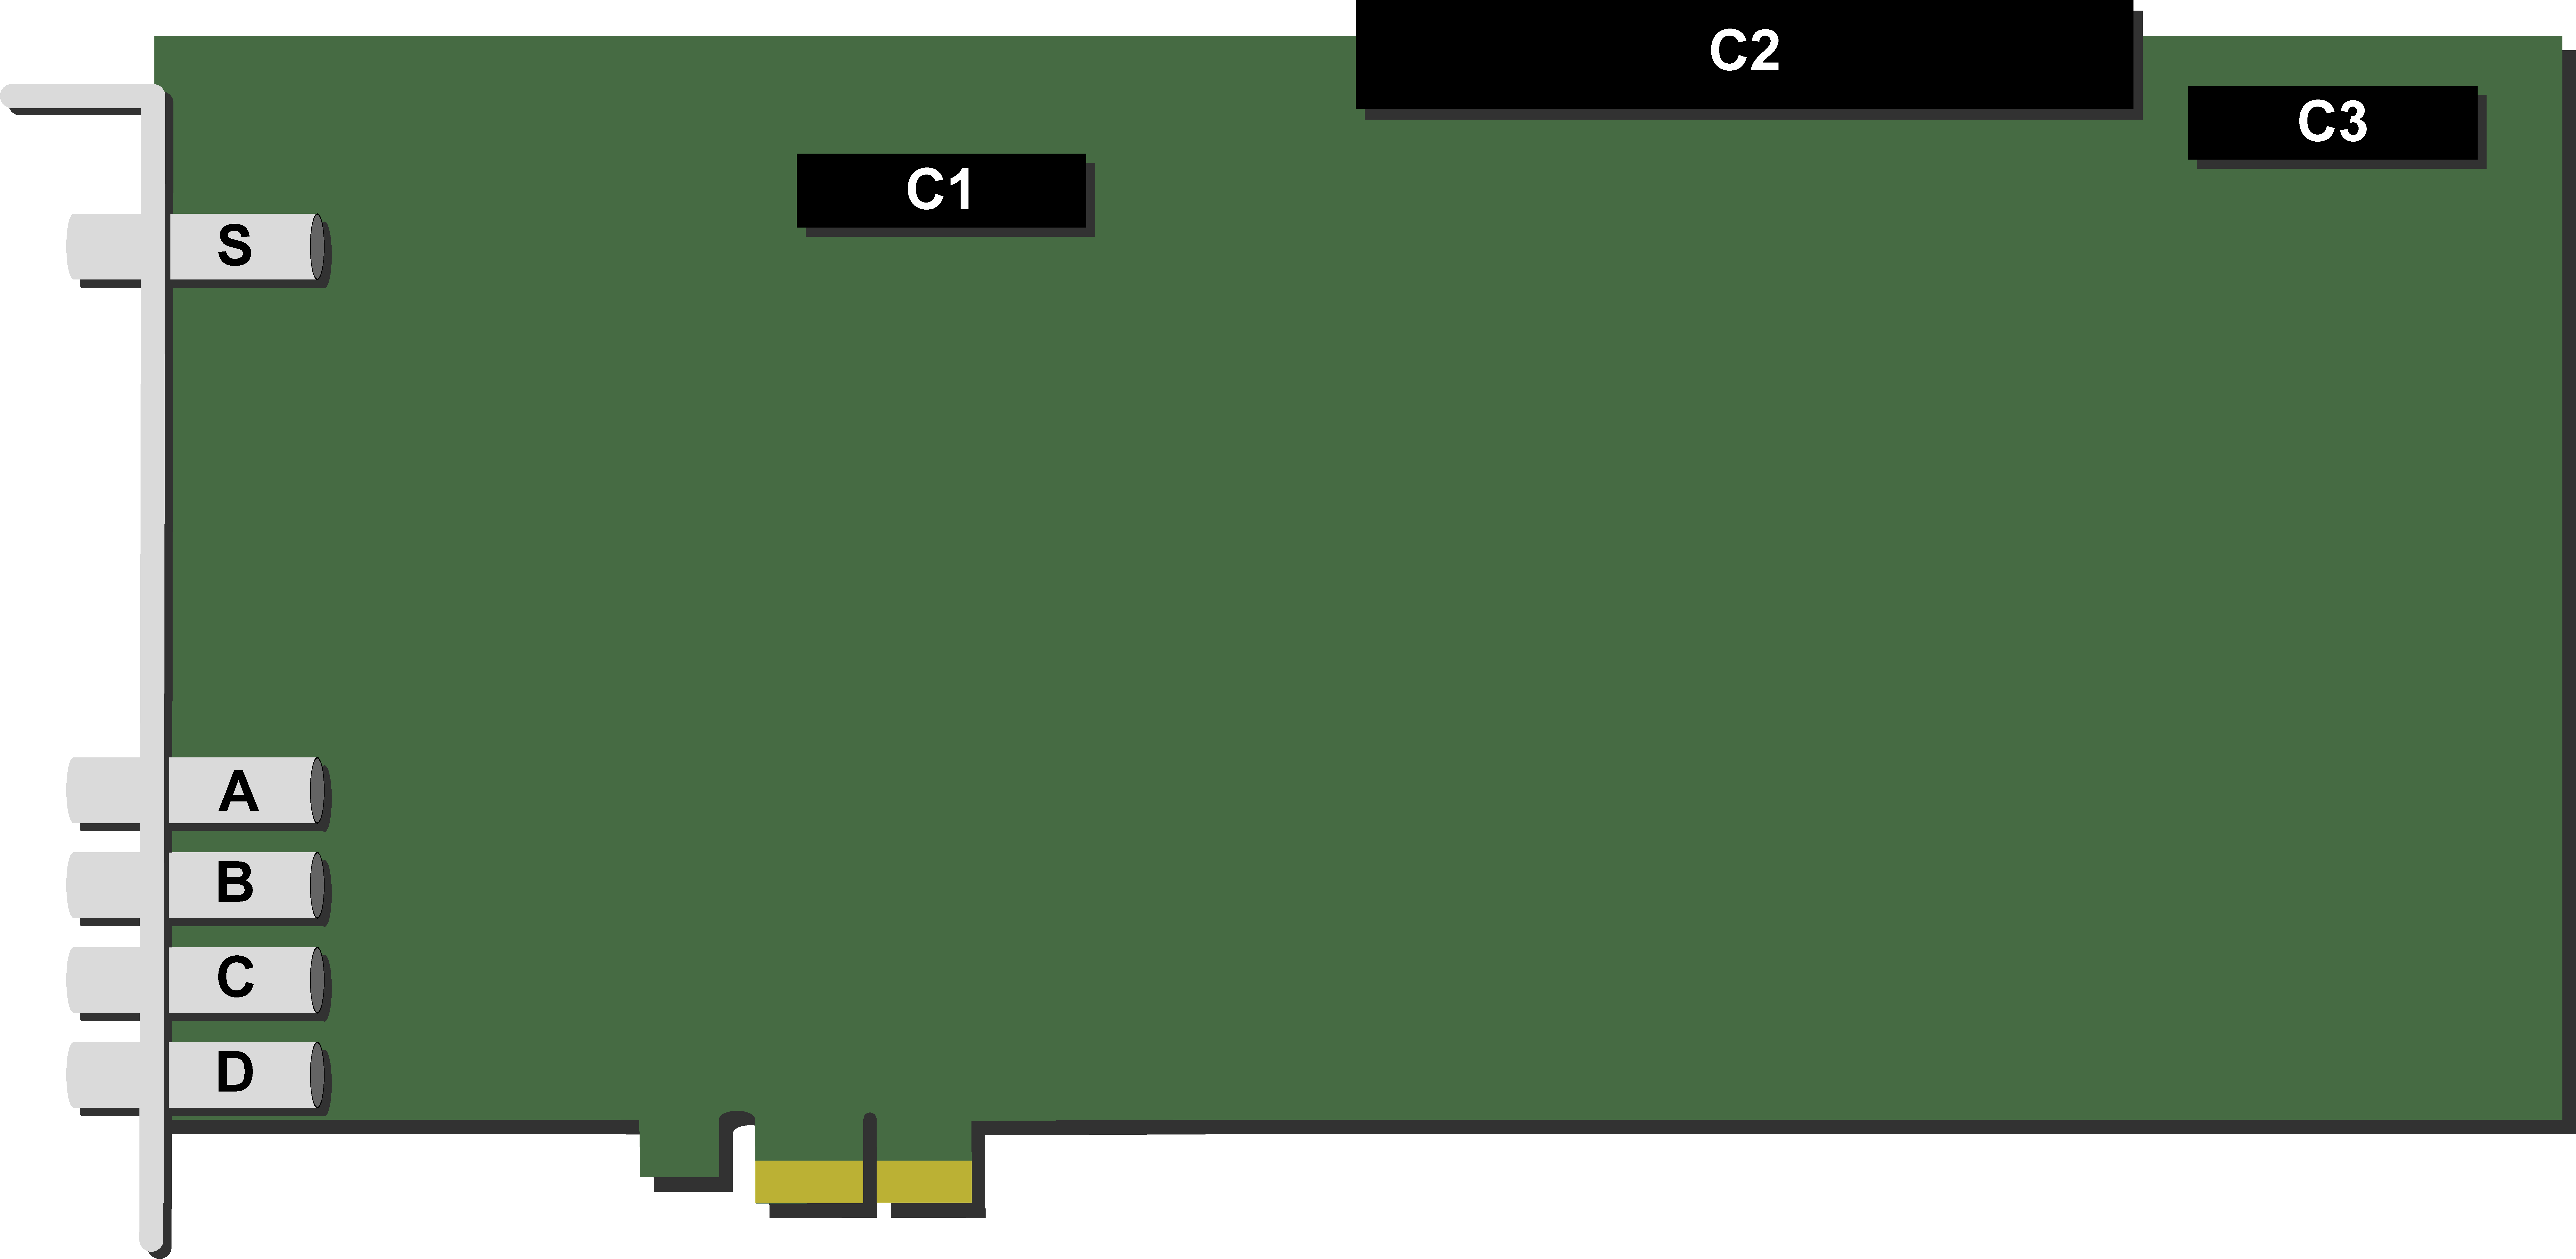
\includegraphics[width=0.7\textwidth]{figures/xTDC4_schematic.pdf}
				}
				
				\caption{Schematic view of a \deviceName\ board showing the inter-board connectors.\label{fig:schematics}}
			\end{center} 
		\end{figure*}
	%

	Furthermore, three inter-board connectors can be found at the top edge of the \deviceName\ board, 
	as displayed in Figure \ref{fig:schematics}. 
	Connector J25 is reserved for future use. The pinout of connector J12 is shown in Table \ref{J12} and the pinout of connector J6 is depicted in Table \ref{J6}.
	\ifxHPTDC{Connector J2 is a coax clock input that must receive a 10 MHz clock if multiple boards are used in together as described in section \ref{multiboard}.}{}

	\begin{table}
	\begin{small}
		\begin{center}
			\begin{tabular}{|c|c|}
				\hline
				Pin & Name\\
				\hline\hline
				1, 2 & GND\\
				\hline
				3, 4 & external CLK in N, external CLK in P\\
				\hline
				5, 6 & GND\\
				\hline
				7, 8 & reserved/NC\\
				\hline
				9, 10 & GND\\
				\hline
				11, 12 & reserved/NC\\
				\hline
				13, 14 & GND\\
				\hline
				15, 16 & reserved/NC\\
				\hline
				17, 18 & GND\\
				\hline
				19, 20 & reserved/NC\\
				\hline
				21, 22 & GND\\
				\hline
				23, 24 & reserved/NC\\
				\hline
				25, 26 & GND\\
				\hline
				27, 28 & reserved/NC\\
				\hline
				29, 30 & GND\\
				\hline
				31, 32 & reserved/NC\\
				\hline
				33, 34 & GND\\
				\hline
			\end{tabular}
			\caption{Pinout of connector J12.}
			\label{J12}
		\end{center}
	\end{small}
	\end{table}

	\begin{table}
	\begin{small}
		\begin{center}
			\begin{tabular}{|c|c|}
				\hline
				Pin & Name\\
				\hline\hline
				1 & +3.3 V\\
				\hline
				2 - 9 & reserved/NC\\
				\hline
				10 & GND\\
				\hline
			\end{tabular}
			\caption{Pinout of connector J6.}
			\label{J6}
		\end{center}
	\end{small}
	\end{table}

%%%%%%%%%%%%%%% multiboard
\ifxHPTDC{
	\section{Synchronizing multiple boards}
		\label{multiboard}
		If more than eight TDC inputs are required, up to eight boards can be synchronises within a system. 
		
		The \deviceName\ API described in chapter \ref{cp:api} manages up to eight boards automatically
		and provides a single data stream that contains sorted hit data from all boards in chronological order. 
		Channel A of each board is assigned channel number \textsf{board\tu index} $\cdot 10$. 
		The \textsf{board\tu index} is assigned to the boards in the order of the serial numbers starting at 0.

		\subsection{Connecting multiple boards}
			The boards must each receive a common 10~MHz clock on connector J2. The connector is inside the PC enclosure. 
			Connectors J12 of all boards must be connected with a flat band cable with a terminator at each end. 
			Cable and Terminator are available from cronologic. See figure \ref{fig:multiboard} for a wiring example.
			%
			\begin{figure*}[ht]
				\begin{center}
					\includegraphics[width=1\textwidth]{xhptdc/figures/multiboard.pdf}				
					\caption{Synchronising multiple boards with a ClockBox.\label{fig:multiboard}}
				\end{center} 
			\end{figure*}
			%
		\subsection{ClockBox}
			For systems of up to four boards cronologic offers the ClockBox product that conveniently makes four clock signals evailable 
			inside the PC enclosure. For use with the \deviceName, jumper JP3 of the CLockBox must be set as shown in Figure \ref{fig:clockbox} to set the clock frequency to 10~MHz. 
			%
			\begin{figure*}[ht]
				\begin{center}
					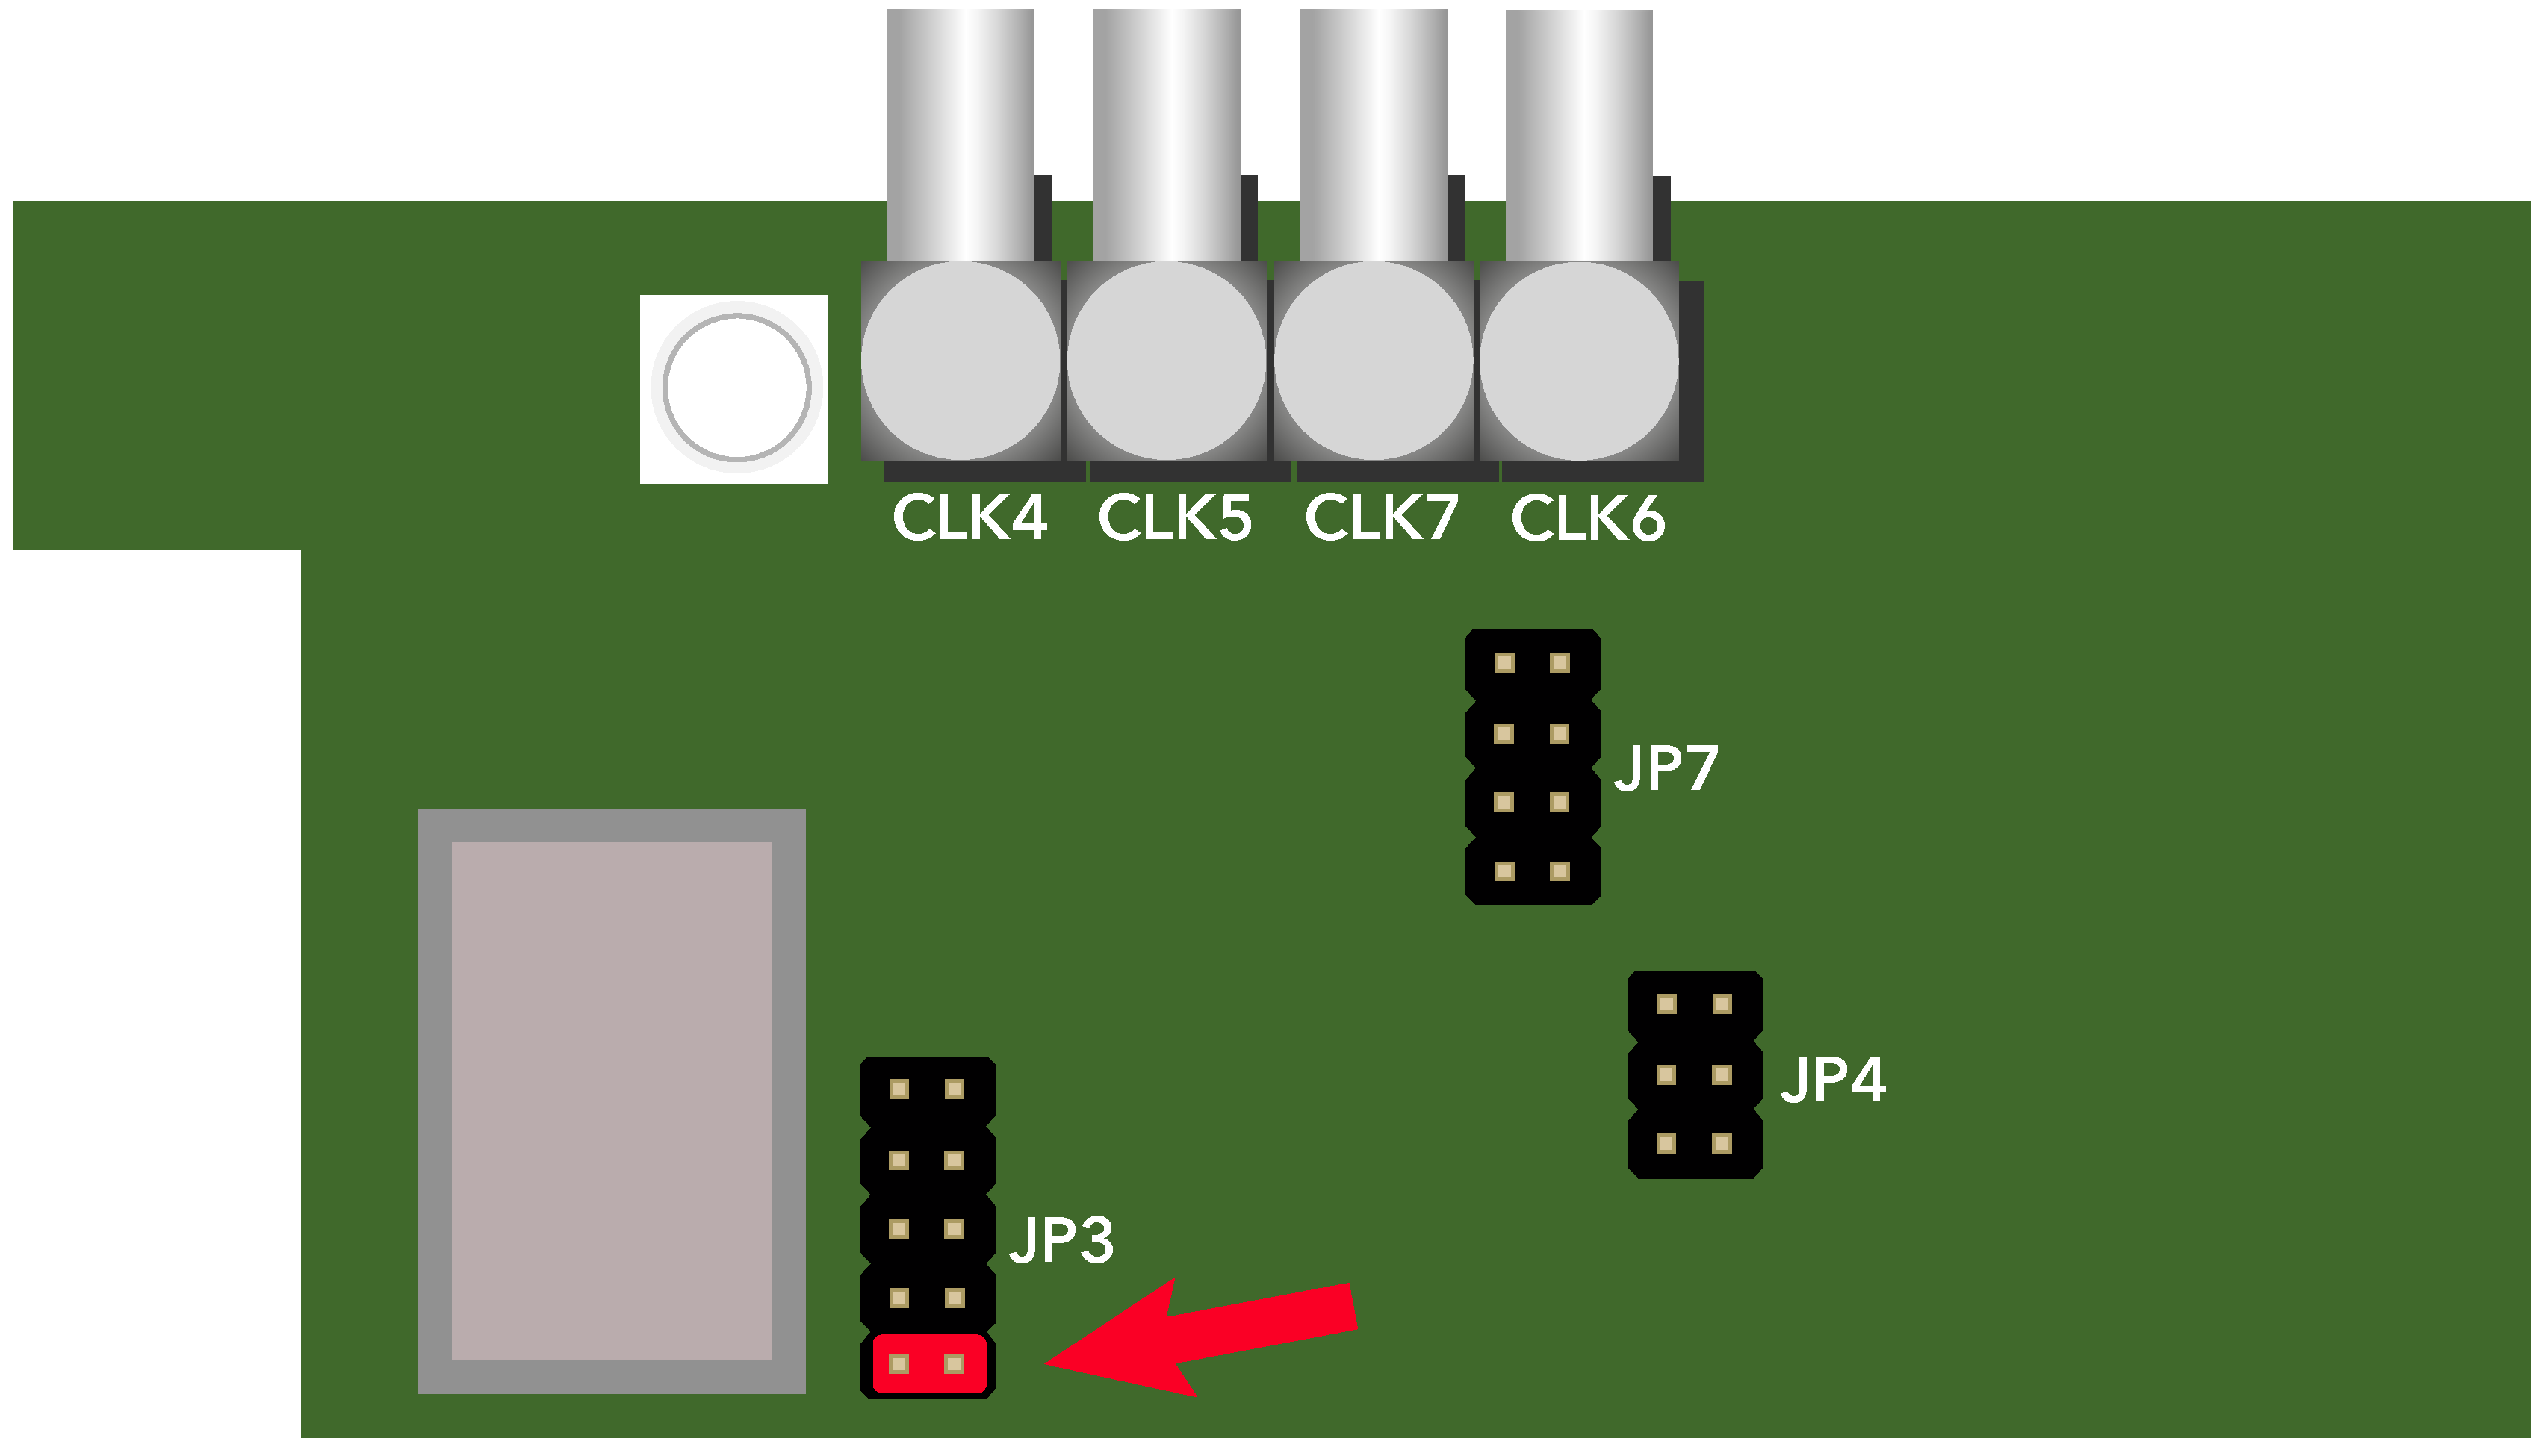
\includegraphics[width=0.5\textwidth]{xhptdc/figures/clockbox.pdf}				
					\caption{ClockBox jumper setting for 10~MHz.\label{fig:clockbox}}
				\end{center} 
			\end{figure*}
			%
		
		\subsection{Crates for multiple boards}
			Most PC mainboards don't have enough PCIe slots to support eight \deviceName s. 
			We offer external enclosure called "Ndigo Crate" that PCIe-over-cable technology to extend the number of available slots in a system.
			The extension is fully transparent to the host system. There are no additional drivers require. 
			Please see the \href{https://www.cronologic.de/products/pcie/pcie-crates}{product page} at our website \url{www.cronologic.de}.  
		

	

}{}




	




	\chapter{\deviceName\ Functionality}
		\txh{ %TimeTagger Version
The \deviceName\ is a ``classic'' common start time-to-digital converter. 

It records the time difference between a leading or trailing edge on the start input to the leading and trailing edges of the stop inputs. 
Rising and falling edges of the stop channel A-D can be enabled individually. 
The measurements are quantized to $500$~ps for -2G devices and tp $1000$~ps for -1G devices. 
The timestamps are recorded in integer multiples of a bin size of $500$~ps for both board types to simplifiy setups where data from differnt board types is combined.
Transitions of the input signals are called hits. To reliably detect hits the signal has to be stable for more than one quantisation interval before and after the edge.  
Triggers on the start channel must not occur less than 5ns apart. The \deviceName\ records events without dead time at a readout rate of about 48MHits/s.
} { %xTDC4 Version
The \deviceName\ is a ``classic'' common start time-to-digital converter. 

It records the time difference between leading or trailing edges on the start input and the stop inputs. 
Each stop channel A-D can be enabled individually. 
The standard deviation of the timestamps is approx. $8$~ps. 
The timestamps are recorded in integer multiples of a bin size of $5/(3\cdot 128) = 13.0208\overline{3}$~ps. 
The data acquisition can be limited to rising or falling signal transitions. 

The maximum trigger rate on the start channel is 4~MHz.

\subsection{Handling of Difficult Hits}
    \label{difficulthits}
    Transitions of the input signals are called hits. To measure all hits with the maximum resolution the hits must fulfill all criteria set forth in this document.
    However, the \deviceName does include mechanisms to provide as much information as possible for hits that fall out of these specs.

    To reliably detect hits the signal has to be stable for at least $900$~ps before and after the edge that is to be measured. 
    Pulses as short as $250$~ps are usually detected at full resolution but have a significant chance to be assigned to the wrong group or appear out of order. 
    For these hits bit 7 in the data word is set. See section \ref{flags} for more information on the data format.

    Between multiple hits on a stop channel a deadtime of approximately $5$~ns is required for full resolution. 
    Hits that are closer together will only be reported with a resolution of $5/6~ns = 833,\overline{3}~ps$. For these hits both bits 6 and 7 are set.

    Data is copied from the 15-entry L0 FIFO to the larger downstream FIFOs at a reate of about $12$~MHz per channel. 
    If the L0 FIFO overflows the hig resolution measurement of some hits will be discarded. 
    In this case a measurement from an alternative TDC wil be used that has a resolution of about $150$~ps. 
    For these hits bit 6 in the data word will be set
} { %xHPTDC8 version
    The \deviceName\ is a streaming time-to-digital converter. It records the timestamps of changes at the inputs A-H in an infinite stream. 
    A flexible grouping mode is available that can emulate common-start or common-stop behaviour. See section \ref{grouping} for details.

    For each channel it can be selected individually whether rising or falling edges are recorded. It is not possible to record both edges of the same channel. 
    The timestamps are recorded in integer multiples of a bin size of $5/(3\cdot 128) = 13.0208\overline{3}$~ps. 
    There must be at least 5~ns between consecutive hits on the same input channel to be detected reliably. 
    The \deviceName\ records events without dead time at a readout rate of about 48MHits/s.
} 
		\section{Grouping and Events}
\label{grouping}
\ifxHPTDC{
    If \textsf{config.tdc\tu mode} is set to \textsf{\PREFIX TDC\tu MODE\tu GROUPING} the TDC will operate in grouping mode. 
    In grouping mode each call to \textsf{xhptdc8\tu read\tu hits()} will return a group of timestamps relative to some trigger event. 
    Otherwise the call returns all available timestamps as absolute timestamps counting upwards from \textsf{xhptdc8\tu start\tu capture()}
}{} 

In typical applications a start hit is followed by a multitude of hits on e.g. a detector. 
The hits recorded are managed in groups (which are called ``events'' in some applications). 
%
\begin{figure*}[ht]
    \begin{center}
        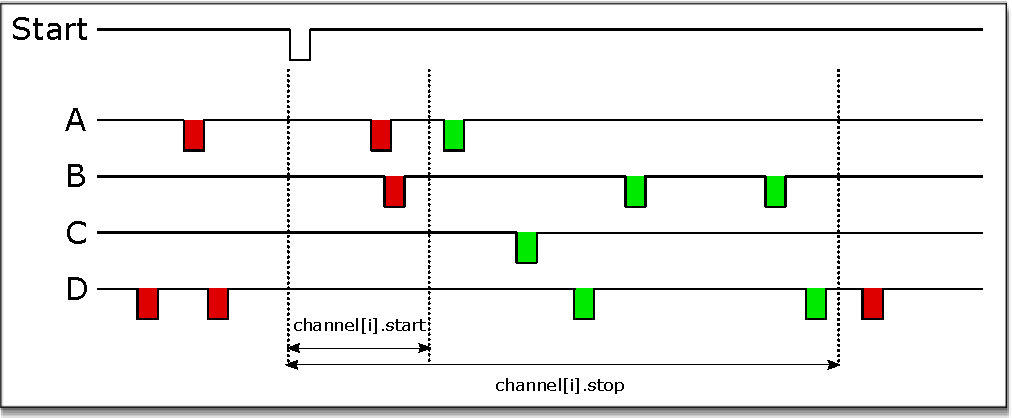
\includegraphics[width=0.7\textwidth]{figures/grouping.pdf}
        \caption{Acquired hits are merged to groups as explained in the text.\label{fig:grouping}}
    \end{center}
\end{figure*}
%

Figure \ref{fig:grouping} shows a corresponding timing diagram. The user can define the range of a group, i.e. the time window within which hits 
on the stop channels are recorded, in software. Hits occurring outside of that time window are discarded. 
 Different ranges can be set for each of the 4 stop channels by setting corresponding values for \textsf{config.grouping.start} and \textsf{.stop} values.

 \ifxHPTDC{
     The values are configured in picoseconds. Negative values can be used in common stop applications.
     \[ -2^{31} <= start <= stop <= 2^{31}-1 \]
 }{
    The values need to be set as multiples of the bin size and must not be negative.
    \[ 0 <= start <= stop <= 2^{16}-1 \]
 }

 In single board setups it is recommended to also configure the gating blocks accordingly. 
 This prevents data from beeing read out that is discarded by the grouping code anyway. 
 Plase note that the grouping parameters are given in picoseconds while the gating blocks are configured in cycles of the 150~MHz clock.


		\lstset{
	language=[Visual]C++,
	keywordstyle=\bfseries\sffamily\color[rgb]{0,0,1},
	identifierstyle=\sffamily,
	commentstyle=\color[rgb]{0.133,0.545,0.133},
	stringstyle=\sffamily\color[rgb]{0.627,0.126,0.941},
	showstringspaces=false,
	basicstyle=\small,
	numberstyle=\footnotesize,
	numbers=left,
	stepnumber=1,
	numbersep=10pt,
	tabsize=2,
	breaklines=true,
	prebreak = \raisebox{0ex}[0ex][0ex]{\ensuremath{\hookleftarrow}},
	breakatwhitespace=false,
	aboveskip={1.5\baselineskip},
	columns=fixed,
	upquote=true,
	extendedchars=true,
}

\section{Auto Triggering Function Generator\label{cp:AutoTriggeringFunctionGenerator}}
Some applications require internal periodic or random triggering. The \deviceName\ function generator provides this functionality.\par

The delay between two trigger pulses of this trigger generator is the sum of two components: A fixed value M and a pseudo random value given by the exponent N. \par

The period is

\begin{align}
    T = 1 + M + [1...2^N]
\end{align}

clock cycles \ifxHPTDC{of the 150~MHz clock}{with a duration of $4~ns$ per cycle}.\par

The trigger can be used as a source for the TiGer unit (see Section \ref{cp:tiger}).


\section{Timing Generator (TiGer)\label{cp:tiger}}
Each digital LEMO-00 input can be used as a \ifxHPTDC{AC coupled}{LVCMOS} trigger output. 
The TiGer function can be configured independently for each connector. 
See Section \ref{cp:tigerblock} for a full description of the configuration options.
% 
\begin{figure*}[ht]
    \begin{center}
        \ifxHPTDC { 
            % this is an XCIrcuit drawing  convertex from postscript with 
            %ps2pdf.exe -dEPSCrop xhptdc8_trigger_matrix.ps
            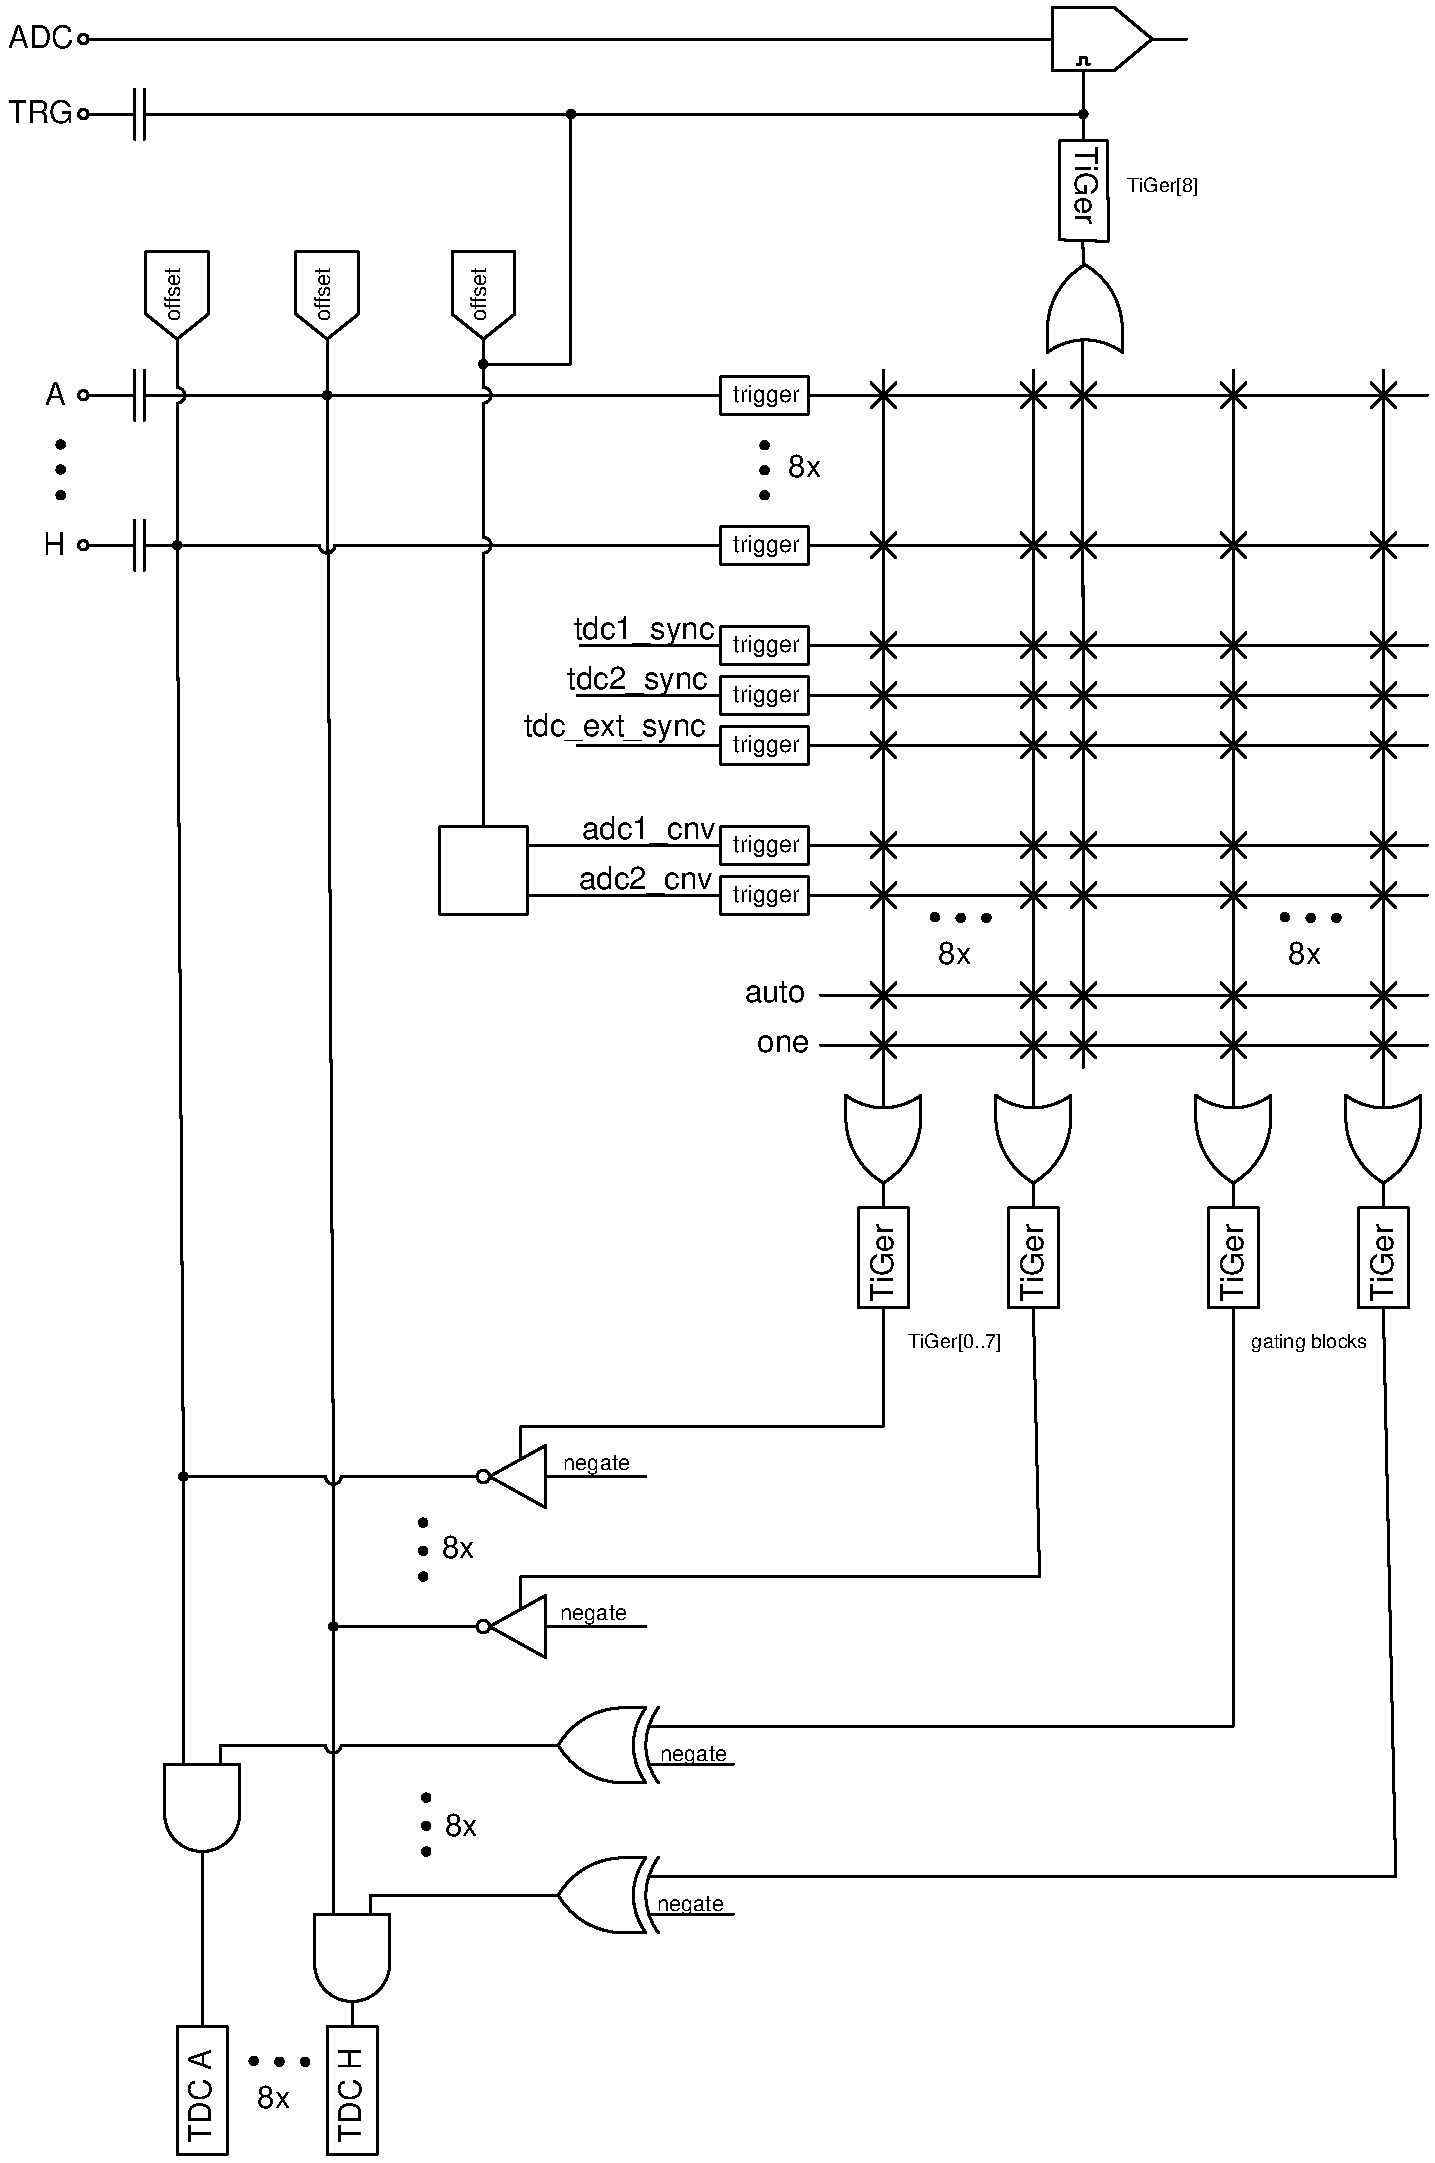
\includegraphics[width=0.6\textwidth]{xhptdc/figures/xhptdc8_trigger_matrix.pdf}
        }{
            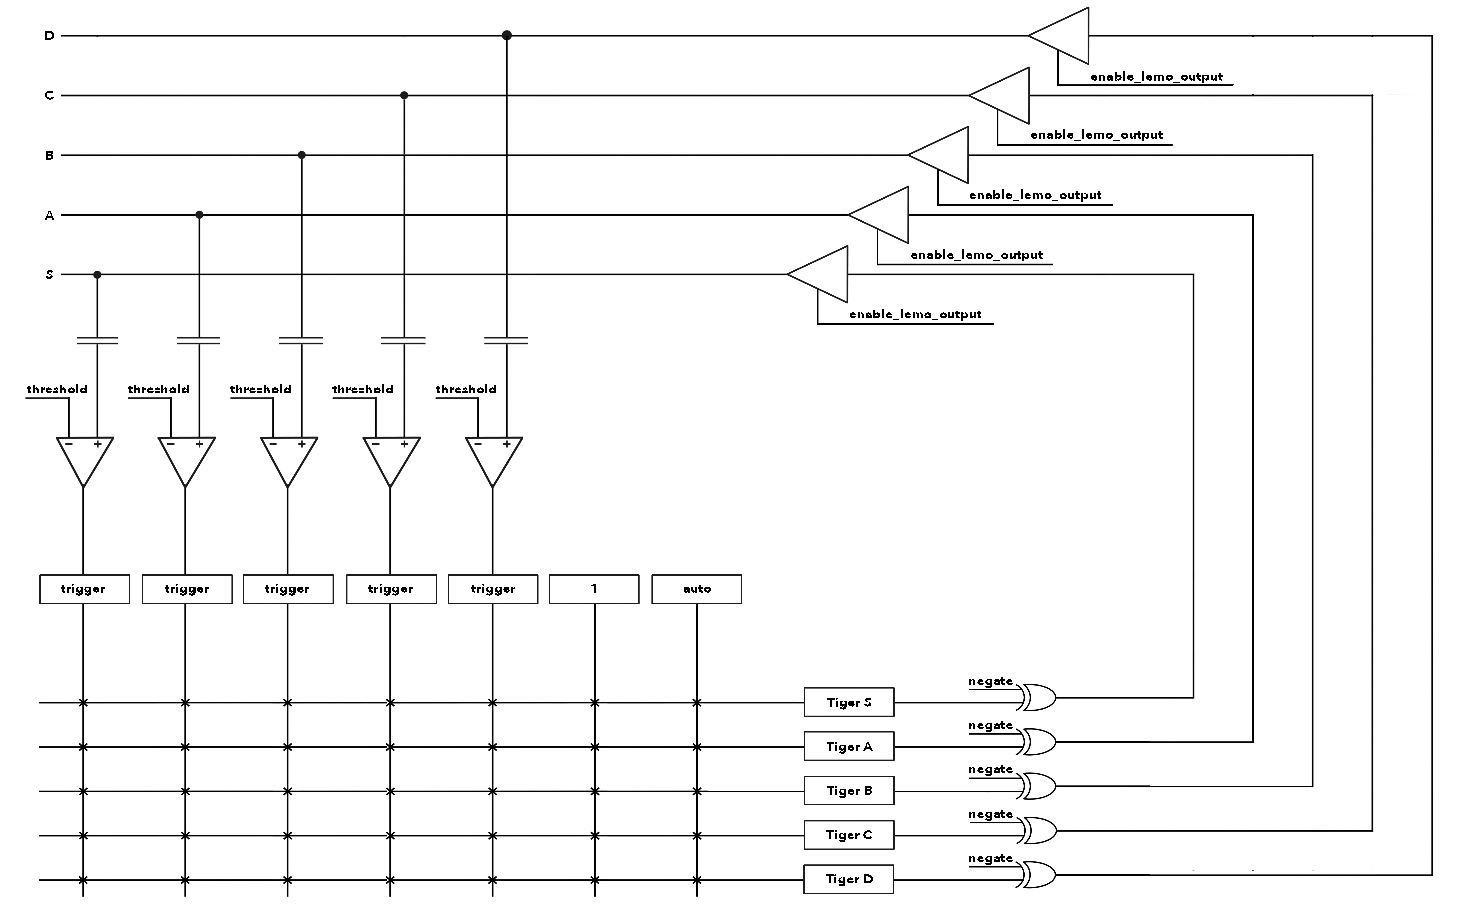
\includegraphics[width=0.7\textwidth]{figures/xTDC4_tiger_matrix.pdf}
        }
        \caption{TiGer blocks can generate outputs that are also available on inputs.\label{fig:matrix}} 
    \end{center}
\end{figure*}
%

Figure \ref{fig:matrix} shows how the TiGer blocks are connected. They can be triggered by an OR of an arbitrary combination of inputs, 
including the auto trigger. Each TiGer can drive its output to its corresponding LEMO connector. This turns the connector into an output. 

When there is an ADC trigger pulse on the TRG connector, either of the two on board ADCs is triggered in an unpredictable pattern. 
If the TRG input shall be used as a trigger the trigger sources must be contain both \textsf{ADC1\tu CNV} and \textsf{ADC21\tu CNV}.

The trigger sources with names ending in \textsf{\tu sync} are managed by the driver for multi board setups and must be left unchanged by the user.

\ifxHPTDC{
	The TiGer outputs are AC coupled to the connector. They can be operated in one of the following modes:
	\paragraph*{\textsf{\PREFIX TIGER\tu OFF}} 
		No signal is output to the connetor. 
	\paragraph*{\textsf{\PREFIX TIGER\tu OUTPUT}} 
		In this mode the connector is input only. Pulses are unipolar with 2V amplitude. 
		Connected hardware must not drive any signals to connectors used as outputs, as doing so could damage both the \deviceName and the external hardware. 
		We recommend to only use short pulses to avoid undesirable baseline shift due to the AC coupling, but the device does not pose any restrictions on the duty cycle. 
		This mode can be used as a clock output with a frequency of $75/N$~MHz for integer $N$.
	\paragraph*{\textsf{\PREFIX TIGER\tu BIDI}} 
		In this mode the TiGer creates unipolar pulses with 1~V amplitude. The connector can still be used as an input. 
		Use short pulses to keep the propability of collision and the effect on the baseline low.	
	\paragraph*{\textsf{\PREFIX TIGER\tu BIPOLAR}} 
		In this mode the connector creates bipolar pulses with 1~V amplitude. The connector can still be used as an input. 
		The pulses have no effect on the baseline offset. 
		TiGer should be configured with $stop = start$ for minimum width bipolar pulses of $2 \times 6.\overline{6}~ns$. 
		The maximum bipolar pulse width is \textsf{XHPTDC8\tu TIGER\tu MAX\tu BIPOLAR\tu PULSE\tu LENGTH = 15}.    
}{
	The TiGer is DC coupled to the connector. Connected hardware must not drive any signals to connectors used as outputs, 
	as doing so could damage both the \deviceName\  and the external hardware.
	Pulses that are short enough for the input AC coupling are available as input signals to the \deviceName. 
	This can be used to measure exact time differences between the generated output signals and input signals on other channels.
}
\ttinput{Tiger_Example.tex}	

\ifxHPTDC{
	\subsection{Triggering the ADC with the TiGer}
		\label{adctiger}
		There is a ninth TiGer that is connected to the trigger input of the ADC. See section \ref{adc} for additional information on the ADC. 

		The ADC TiGer can be used with retrigger enabled to periodically sample ADC data. 
		The period should be no shorter than 300~ns or 45 TiGer clocks.

		The ADC TiGer can also be used to sample voltages at a time relative to one of the TDC inputs. In this case 
		stop should be set to at least 45 to ensure that the sample period criterion is met even when pulses
		arrive in quick succession. A typical application would be to sample some slow control voltage once per start signal.

	\section{Gating}
		Each TDC channel has a second TiGer block that functions as a gate as shown in figure \ref{fig:matrix}. 
		While that output of that gating block is active no hits are recorded in that channel.
		If the block is negated hits are only recorded while the gating block is active.
		
		This is a useful feature in setups where the trigger creates a lot of noise.
		A suitable configuration of the gating block can reduce the bandwidth and buffer usage significantly.
		Gating is performed before the L0 buffer. Grouping is performed in software after readout. 
		
	\section{Triggerable ADC}
		\label{adc}
		The \deviceName\ is equipped with a triggerable ADC. 
		Whenever there is a rising edge on the ADC trigger connector, 
		the voltage on the ADC input connector is sampled. 
		The result is inserted as a packet with timestamp and ADC value into the readout data stream.

		The ADC trigger also is connected to the output of a TiGer block. 
		This can be used to to trigger the ADC periodical or relative to one of the TDC input as described in section \ref{adctiger}

		The ADC triggers should not be closer than 300ns apart.

		There are two interleaved ADCs  to ensure that there is always an ADC available even during readout. 
		This is exposed to the user both in the output data format and in the TiGer and Gating trigger sources.
		When using the ADC trigger as a trigger for Gating or TiGer both trigger sources shall be set to the same value.
		During readout the user shall not distinguish between data from the two ADCs unless advanced calibration is 
		desired for the ADC data. In that case the two ADCs should be treated separately.   

}{} 

	\chapter{Driver Programming API\label{cp:api}} 
		% also includes common/StructConfig.tex and common/InfoStructs.tex
		\ifxHPTDC{
	\newcommand{\device}{\cronvar{\prefix manager}{*xhptdc8\tu mgr}}
	\newcommand{\deviceindex}{\device, \cronvar{int}{index}}
	\newcommand{\deviceconfig}{\device}
	\newcommand{\initparameters}{xhptdc8manager\tu init\tu parameters}
}{
	\newcommand{\device}{\cronvar{\prefix device}{*device}}
	\newcommand{\deviceindex}{\device}
	\newcommand{\deviceconfig}{\deviceindex}
	\newcommand{\initparameters}{\prefix init\tu parameters}
}

The API is a DLL with C linkage.\par

The functions provided by the DLL are declared in \textsf{\txh{TimeTagger4}{xTDC4}{xHPTDC8}\tu interface.h}.

\section{Constants}
\ifxHPTDC{
	\crondef{XHPTDC8MANAGER\tu DEVICES\tu MAX 8}\\
	The maximum number of boards supported by the device manager.

	\ttdef{TDC\tu CHANNEL\tu COUNT 8}\\
	The number of TDC input channels.\par

	\ttdef{GATE\tu COUNT 8}\\
	The number of gating blocks. One for each TDC input.\par

	 \ttdef{TIGER\tu COUNT 9}\\
	The number of timing generators. One for each TDC input and one for the adc trigger.\par

	 \ttdef{TRIGGER\tu COUNT 16}\\
	The number of potential trigger sources for the timing generators. One for each TDC input 
	\ifxHPTDC{}{, one for the Start input} plus some specials. 
	 See Section~\ref{cp:tigerblock} for details.\par

}{ 
	\ttdef{CHANNEL\tu COUNT 4}\\
	The number of TDC input channels.\par

	 \ttdef{TIGER\tu COUNT 5}\\
	The number of timing generators. One for each TDC input and one for the start input.\par

	 \ttdef{TRIGGER\tu COUNT 16}\\
	The number of potential trigger sources for the timing generators. One for each TDC input, one for the Start input plus some specials. 
	 See Section~\ref{cp:tigerblock} for details.\par
}


\section{Driver Information}

	Even if there is no board present the driver revision can be queried using these functions.

	\ttvar{int}{get\tu driver\tu revision()}\\
	Returns the driver version, same format as \textsf{\prefix static\tu info.driver\tu revision}. 
	This function does not require a \deviceName\ board to be present.

	\ttvar{const char*}{get\tu driver\tu revision\tu str()}\\
	Returns the driver version including SVN build revision as a string. 

	\ttvar{int}{count\tu devices(}\cronvar{int}{*error\tu code}, \cronvar{char}{**error\tu message)}\\
	\label{countdevices}
	Returns the number of boards present in the system that are supported by this driver.\par


\section {Initialization}

		\ttvar{int}{close(}\device )\\
		Finalizes the driver for this device.

		\ttvar{int}{get\tu default\tu init\tu parameters(}\cronvar{\initparameters}{ *init)}\\
		Sets up the standard parameters. Gets a set of default parameters for \textsf{\prefix init()}. This must always be used to initialize the \textsf{\prefix init\tu parameter()} structure.\par

		\cronvar{\prefix \ifxHPTDC{manager}{device} *}{\prefix init(}\cronvar{\initparameters}{*params}, \\ 
		\cronvar{int}{*error\tu code}, \cronvar{char}{**error\tu message)}\\
		Opens and initializes the \deviceName\ board with the given index. 
		The user must provide pointers to memory locations where the driver can store return values.\\
		\textsf{error\tu code} shall point to an integer for the error code. \\
		\textsf{error\tu message} must point to a pointer to char. The driver will allocate a buffer for zero terminated error messages and store the address of the buffer in the location provided by the user.\par

		The paramter \textsf{params} is a structure of type \textsf{\prefix init\tu parameters} that must be completely initialized.\par

%%%%%%%%%%%%%%%%% struct init_parameters

		\subsection{Structure \initparameters}
			\cronvar{int}{version}\\
			The version number. Must be set to \textsf{\PREFIX API\tu VERSION}.\par

			\ifxHPTDC{}{
				\cronvar{int}{card\tu index}\\
				The index in the list of \deviceName\ boards that should be initialized.\\
				There might be multiple boards in the system that are handled by this driver as reported by \textsf{\prefix count\tu devices}. This index selects one of them. Boards are enumerated depending on the PCIe slot. 
				The lower the bus number and the lower the slot number the lower the card index.\par

				\cronvar{int}{board\tu id}\\
				the global index in all cronologic devices.\\
				This 8 bit number is filled into each packet created by the board and is useful if data streams of multiple boards will be merged. If only \deviceName\ cards are used this number can be set to the \textsf{card\tu index}. 
				If boards of different types that use a compatible data format are used in a system each board should get a unique id.
				Can be changed with \textsf{int \prefix set\tu board\tu id\allowbreak(\prefix device *device, int board\tu id)}.\par
			}

			\cronvar{\tu \tu int64}{buffer\tu size\ifxHPTDC{}{[8]}}\\
			The minimum size of the DMA buffer.\\
			If set to 0 the default size of 16~MByte is used. 
			\ifxHPTDC{}{For the \deviceName\ only the first entry is used.}\par

			\ifxHPTDC{}{
				\cronvar{int}{buffer\tu type}\\
				The type of buffer. Must be set to 0.
				\begin{description}
					\item[]  \ttdef{BUFFER\tu ALLOCATE   0}
					\item[]  \ttdef{BUFFER\tu USE\tu PHYSICAL   1}  // unsupported
				\end{description}
			

				\cronvar{\tu \tu int64}{buffer\tu address}\\
				This is set by \prefix init() to the start address of the reserved memory.\\ 
				The buffers will be allocated with the sizes given above. Make sure that the memory is large enough.\par
			}

			\cronvar{int}{variant}\\
			Set to 0. Can be used to activate future device variants such as different base frequencies.\par

			\cronvar{int}{device\tu type}\\
			A constant for the different devices of cronologic \textsf{CRONO\tu DEVICE\tu *}.\\
			Initialized by \textsf{\prefix get\tu default\tu init\tu parameters()}. This value is identical to the PCI Device ID. Must be left unchanged.

			\begin{tabular}{ll}
				\crondef{CRONO\tu DEVICE\tu HPTDC}       & 0x1 \\
				\crondef{CRONO\tu DEVICE\tu NDIGO5G}     & 0x2 \\
				\crondef{CRONO\tu DEVICE\tu NDIGO250M}   & 0x4 \\
				\crondef{CRONO\tu DEVICE\tu xTDC4}       & 0x6 \\
				\crondef{CRONO\tu DEVICE\tu TIMETAGGER4} & 0x8 \\
				\crondef{CRONO\tu DEVICE\tu XHPTDC8}     & 0xC \\
				\crondef{CRONO\tu DEVICE\tu NDIGO6}      & 0xD \\
			\end{tabular}

			\cronvar{int}{dma\tu read\tu delay}\\
			The update delay of the write pointer after a packet has been sent over PCIe. Specified in multiples of 16~ns.
			Should not be changed by the user.\par

			\ifxHPTDC{
				\cronvar{int}{multiboard}\\
				Set if multiple devices shall be synchronized.\par
	
				\cronvar{int}{use\tu ext\tu clock}\\
				If set to 1 use external 10 MHz reference. If set to 0 use internal reference.\par

				\cronvar{int}{ignore\tu calibration}\\
				Leave at 0 to use device calibration data.\par
		
			}{
				\cronvar{int}{use\tu ext\tu clock}\\
				If set to 1 use external 10 MHz reference. If set to 0 use internal reference.\par	
			}
	

	
	% info structures
	\section{Status Information}
	

\subsection{Functions for Information Retrieval}
    The driver provides functions to retrieve detailed information on the board type, its configuration, settings and state. 
    The information is split according to its scope and the computational requirements to query the information from the board.
    
    \ifxHPTDC{
        The information is provided on a per board basis. The parameter \textsf{index} selects which board is queried.
    }{}

    \ttvar{int}{get\tu device\tu type}(\device)\\
    Returns the type of the device as \textsf{CRONO\tu DEVICE\tu \txh{TIMETAGGER4}{XTDC4}{XHPTDC8}}.\par

    \ttvar{const char*}{get\tu last\tu error\tu message(\device)}\\
    Returns most recent error message.\par

    \ttvar{int}{get\tu fast\tu info(}\deviceindex, \lb\cronvar{\prefix fast\tu info}{*info)}\\
    Returns fast dynamic information.\\
    This call gets a structure that contains dynamic information that can be obtained within a few microseconds.\par

    \ttvar{int}{get\tu param\tu info(}\deviceindex, \lb\cronvar{\prefix param\tu info}{*info)}\\
    Returns configuration changes.\\
    Gets a structure that contains information that changes indirectly due to configuration changes.\par


    \ttvar{int}{get\tu static\tu info(}\deviceindex, \lb\cronvar{\prefix static\tu info}{*info)}\\
    Contains static information.\\
    Gets a structure that contains information about the board that does not change during run time.\par 

   \ifxHPTDC{
        \ttvar{int}{get\tu temperature\tu info(}\deviceindex, \lb\cronvar{\prefix temperature\tu info}{*info)}\\
        Get temperature measurements from multiple sources on the board.

        \ttvar{int}{get\tu clock\tu info(}\deviceindex, \lb\cronvar{\prefix clock\tu info}{*info)}\\
        Get information on clocking configuration an status.

        \ttvar{const char *}{device\tu state\tu to \tu str(}\cronvar{int state)}\\
        Convert the state value from \textsf{\prefix fast\tu info.state} into a human readable string. 
   }{   
        \ttvar{int}{get\tu slow\tu info(}\deviceindex, \lb\cronvar{\prefix slow\tu info}{*info)}\\
        Returns slow dynamic information.\\
        The data reported in this structure requires milliseconds to be obtained. 
        The application should only call it in situations where the program flow can be blocked as long.\par
   } 

%%%%%%%%%%%%%%%%% static info

\subsection{Structure \prefix static\tu info}

This structure contains information about the board that does not change during run time. It is provided by the function \textsf{\prefix get\tu static\tu info}.\par

\cronvar{int}{size}\\
The number of bytes occupied by the structure.

\cronvar{int}{version}\\
A version number that is increased when the definition of the structure is changed. The increment can be larger than one to match driver version numbers or similar. Currently only version 0 is defined.\par

\cronvar{int}{board\tu id}\\
ID of the board.\\
\ifxHPTDC{
    All \deviceName\ boards in the system are numbered according in order of their serial numbers starting at zero.
    The channel A of a board has channel number $board\_id \cdot 10$. \par
}{}

\cronvar{int}{driver\tu revision}\\
Encoded version number for the driver.\\
The lower three bytes contain a triple level hierarchy of version numbers, e.g. 0x010103 encodes version 1.1.3.\\
The versionen adheres to the Semantic Versioning scheme as defined at \href{https://semver.org}{https://semver.org}. A change in the first digit generally requires a recompilation of user applications. 
Changes in the second digit denote significant improvements or changes that don't break compatibility 
and the third digit increments with minor bug fixes and similar updates that do not affect the API.\par

\cronvar{int}{driver\tu build\tu revision}\\
The build number of the driver according to cronologic's internal versioning system.

\cronvar{int}{firmware\tu revision}\\
Revision number of the FPGA configuration.

\cronvar{int}{board\tu revision}\\
Board revision number.\\
The board revision number can be read from a register. It is a four-bit number that changes when the schematic of the board is changed. This should match the revision number printed on the board.

\cronvar{int}{board\tu configuration}\\
Describes the schematic configuration of the board.\\
The same board schematic can be populated in multiple variants. This is a four bit-code that can be read from a register.

\cronvar{int}{subversion\tu revision}\\
Subversion revision id of the FPGA configuration source code.

\txh{
    \cronvar{int}{chip\tu id}\\
    Reserved.
}{
    \cronvar{int}{chip\tu id}\\
    16 bit factory ID of the TDC chip.
}{
    \cronvar{int}{chip\tu id[2]}\\
    16 bit factory ID for each of the TDC chips.
}\par

\cronvar{int}{board\tu serial}\\
Serial number.\\
With year and running number in 8.24 format. The number is identical to the one printed on the silvery sticker on the board.\par

\cronvar{unsigned int}{flash\tu serial\tu high}\\
\cronvar{unsigned int}{flash\tu serial\tu low}\\
64-bit manufacturer serial number of the flash chip

\cronvar{crono\tu bool\tu t}{flash\tu valid}\\
If not 0 the driver found valid calibration data in the flash on the board and is using it.\par

\cronvar{int}{calibration\tu date}\\
DIN EN ISO 8601 string YYYY-MM-DD HH:DD describing the time when the card was calibrated.

%%%%%%%%%%%%%%%%%%%%%%%% param info

\subsection{Structure \prefix param\tu info}
This struct contains configuration changes provided by \textsf{\prefix get\tu param\tu info()}.

\cronvar{int}{size}\\
The number of bytes occupied by the structure. \par

\cronvar{int}{version}\\
A version number that is increased when the definition of the structure is changed. The increment can be larger than one to match driver version numbers or similar. Currently only version 0 is defined.\par


\cronvar{double}{binsize}\\
Bin size (in ps) of the measured TDC data.

\ifxHPTDC{}{ %board ID is found in the static_info structure.
    \cronvar{int}{board\tu id}\\
    Board ID.\\
    The board uses this ID to identify itself in the output data stream. The ID takes values between 0 and 255.\par
}

\cronvar{int}{channels}\\
Number of TDC channels of the board.\\
Returns \ifxHPTDC{8}{4}.\par

\cronvar{int}{channel\tu mask}\\
Bit assignment of each enabled input channel.\\
Bit $0 \leq n < \ifxHPTDC{8}{4}$ is set if channel $n$ is enabled. \par

\cronvar{\tu\tu int64}{total\tu buffer}\\
The total amount of DMA buffer in bytes.

%%%%%%%%%%%%%%%%%%%%%%%%%% fast info

\subsection{Structure \prefix fast\tu info}
\label{structfastinfo}
\cronvar{int}{size}\\
The number of bytes occupied by the structure. \par

\cronvar{int}{version}\\
A version number that is increased when the definition of the structure is changed. 
The increment can be larger than one to match driver version numbers or similar. 
Currently only version 0 is defined.\par

\ifxHPTDC{} {
    \cronvar{int}{tdc\tu rpm}\\
    Speed of the TDC fan in rounds per minute. Reports 0 if no fan is present.\par
}
\cronvar{int}{fpga\tu rpm}\\
Speed of the FPGA fan in rounds per minute. Reports 0 if no fan is present.\par

\cronvar{int}{alerts}\\
Alert bits from temperature sensor and the system monitor.
\itett{
    The TimeTagger4 does not implement any temperature alerts.
}{
    Bit 0 is set if the TDC temperature exceeds 140°C. 
    In this case the TDC did shut down and the device needs to be reinitialized. 
}\par

\cronvar{int}{pcie\tu pwr\tu mgmt}\\
Always 0. \par

\cronvar{int}{pcie\tu link\tu width}\\
Number of PCIe lanes the card uses. Should always be 1 for the \deviceName. \par

\cronvar{int}{pcie\tu max\tu payload}\\
Maximum size in bytes for one PCIe transaction. Depends on system configuration.\par

\cronvar{int}{state}\\
The state the XHPTDC8Manager is in.

\begin{tabular}{lc}
    \cronvar{const static int}{\PREFIX DEVICE\tu STATE\tu CREATED} & 0  \\*
    \cronvar{const static int}{\PREFIX DEVICE\tu STATE\tu INITIALIZED} & 1  \\*
    \cronvar{const static int}{\PREFIX DEVICE\tu STATE\tu CONFIGURED} & 2  \\*
    \cronvar{const static int}{\PREFIX DEVICE\tu STATE\tu CAPTURING} & 3  \\*
    \cronvar{const static int}{\PREFIX DEVICE\tu STATE\tu PAUSED} & 4  \\*
    \cronvar{const static int}{\PREFIX DEVICE\tu STATE\tu CLOSED} & 5  \\*
\end{tabular}\par

%%%%%%%%%%%%%%%%%%%%%%% temperature info

\ifxHPTDC{
    \subsection{Structure \prefix temperature\tu info}

        \cronvar{int}{size}\\
        The number of bytes occupied by the structure. \par

        \cronvar{int}{version}\\
        A version number that is increased when the definition of the structure is changed. The increment can be larger than one to match driver version numbers or similar. Currently only version 0 is defined.\par

        \cronvar{float}{tdc[2]}\\
        Temperature for each of the TDC chips in °C

        \cronvar{float}{fpga}
        Temperature in °C read from the FPGA's internal sensor.

    %%%%%%%%%%%%%%%%%%%%% clock info

    \subsection{Structure \prefix clock\tu info}

        \cronvar{int}{size}\\
        The number of bytes occupied by the structure. \par

        \cronvar{int}{version}\\
        A version number that is increased when the definition of the structure is changed. The increment can be larger than one to match driver version numbers or similar. Currently only version 0 is defined.\par

        \cronvar{crono\tu bool\tu t}{cdce\tu locked}\\
        Set if the jitter cleaning PLL clock synthesizer achieved lock.

        \cronvar{int}{cdce\tu version}\\
        Version information from the CDCE62005 clock synthesizer.\\
        
        \cronvar{crono\tu bool\tu t}{use\tu ext\tu clock}\\
        Source for the clock synthesizer is usually the 10MHz on board oscillator. During initialisation alternatively  an external clock on J2 can be selected.
        When multiple boards are synchonised all board use a common external clock. See section \ref{multiboard} for details.
        \\       

    
        \cronvar{crono\tu bool\tu t}{fpga\tu locked}\\
        Set if the FPGA datapath PLL achieved lock.\\
    
}{}

	

	\section{Configuration}
		\ifxHPTDC{
			All \deviceName\ boards in the system are configured by a single configuration structure which in turn contains sub structures that configure the individual boards.
		}{
			The device is configured with a configuration structure. 
		}
		The user should first obtain a structure that contains the default settings of the device read from an on-board ROM, 
		then modify the structure as needed for the user application and use the result to configure the device.\par


		\ttvar{int}{configure(}\deviceconfig, \\ \cronvar{\prefix \ifxHPTDC{manager\tu }{}configuration}{*config)}\\
		Configures the \deviceName\ manager.\par

		\ttvar{int}{get\tu current\tu configuration(}\deviceconfig, \\ \cronvar{\prefix \ifxHPTDC{manager\tu }{}configuration}{*config)}\\
		Gets current configuration. Copies the current configuration to the specified config pointer.\par

		\ttvar{int}{get\tu default\tu configuration(}\deviceconfig, \\ \cronvar{\prefix \ifxHPTDC{manager\tu }{}configuration}{*config)}\\
		Gets default configuration. Copies the default configuration to the specified config pointer.\par


	%%%%%%%%%%%%%%%%% configuration structure mostly shared between devices
	%%%%%%%%%%%% struct manager configuration
\ifxHPTDC{
	\subsection{Structure \prefix manager\tu configuration}
	\cronvar{int}{size}\\
	The number of bytes occupied by the structure.\par

	\cronvar{int}{version}\\
	A version number that is increased when the definition of the structure is changed. The increment can be larger than one to match driver version numbers or similar. Currently only version 0 is defined.\par

	\cronvar{\prefix device\tu configuration}{device\tu configs[\PREFIX DEVICES\tu MAX]}\\
	A structure with the configuration for an individual \deviceName\ board as defined in ssection \ref{structconfig}.
	Use the function \textsf{\prefix count\tu devices()} to query how many entries contain valid information. See section \ref{countdevices} for details on the function. \par 

	\cronvar{\prefix grouping\tu configuration}{grouping}\\
	Structure with the parameters for grouping. 
	See section \ref{structgrouping} for the definition of the structure and section \ref{grouping} for more information on grouping.\par

	\cronvar{void}{*bin\tu to\tu ps}\\
	Reserved for future use.
	
}{}
%%%%%%%%%%%%%% struct device_configuration
\subsection{Structure \prefix \ifxHPTDC{device\tu}{}configuration}
	\label{structconfig}
	This is the structure containing the configuration information. 
	\ifxHPTDC{}{ % xHPTDC8 uses TDC manager instead
		It is used in conjunction with \textsf{\prefix get\tu default\tu configuration()}, \textsf{\prefix get\tu current\tu configuration()} and \textsf{\prefix configure()}.\par
	}
	It uses the multiple substructures to configure various aspects of the board. 

	\cronvar{int}{size}\\
	The number of bytes occupied by the structure.\par

	\cronvar{int}{version}\\
	A version number that is increased when the definition of the structure is changed. The increment can be larger than one to match driver version numbers or similar. Currently only version 0 is defined.\par

	% autotrigger was reordered for the xHPTDC so we need to be able to use it in conditionally
	\newcommand{\autotrigger}{			
		\cronvar{int}{auto\tu trigger\tu period}\\
		\cronvar{int}{auto\tu trigger\tu random\tu exponent}\\
		Create a trigger either periodically or randomly. There are two parameters $M = \text{trigger\tu period}$ and $N = \text{random\tu exponent}$ that result in a distance between triggers of $T$ clock cycles.

		\begin{align}
			T &= 1 + M + [1...2^N]\\
			&0 \leq M < 2^{32}\\
			&0 \leq N < 32
		\end{align}

		\noindent There is no enable or reset. The auto trigger is running continously. 
		The usage of this trigger can be configured in the TiGer block source field.\par
	}
	\ifxHPTDC{
		\autotrigger
	}{}

	\ifxHPTDC{ %see xhptdc8_grouping_configuration.enable	
	}{
		\cronvar{int}{tdc\tu mode}\\
		TDC mode. Can be grouped or continuous.
		Currently only \textsf{\PREFIX TDC\tu MODE\tu GROUPED} is supported. 
		This is set per default by \textsf{\prefix get\tu current\tu configuration()} and should be left unchanged.
	}\par

	\ifxHPTDC{} % does not exist for xHPTDC8
	{
		\cronvar{crono\tu bool\tu t}{start\tu rising} 
		\itett{
			Not applicable for the \deviceName.
		}{
			Selects whether the rising or falling edge of the start signal is used to start a group.
		}\par
	}

	\cronvar{double}{threshold[\PREFIX TDC\tu CHANNEL\tu COUNT + 1]}\\	
	Set the threshold voltage for the input channels \ifxHPTDC{A \ldots H and TRG}{S, A \ldots D} (see figure \ref{fig:dcoffset1}).
	\begin{itemize}
		\ifxHPTDC{
			\item threshold[0 - 7] : threshold for channels A \ldots H
			\item threshold[8] : threshold for channel TRG
		}{
			\item dc\tu offset[0] : threshold for channel Start
			\item dc\tu offset[1 - 4] : threshold for channels A \ldots D
		}
	\end{itemize}
	Supported range is -1.32V to +1.18V. This should be close to 50\% of the height of the input pulse. Examples for various signaling standards are defined as follows:\par
	\ifxHPTDC{
		\newcommand{\DCOFFSET}{THRESHOLD\tu}
	}{
		\newcommand{\DCOFFSET}{DC\tu OFFSET\tu}
	}
	\begin{tabular}{ll}
		\ttdef{\DCOFFSET P\tu NIM} & +0.35\\
		\ttdef{\DCOFFSET P\tu CMOS} & +1.18\\
		\ttdef{\DCOFFSET P\tu LVCMOS\tu 33} & +1.18\\
		\ttdef{\DCOFFSET P\tu LVCMOS\tu 25} & +1.18\\
		\ttdef{\DCOFFSET P\tu LVCMOS\tu 18} & +0.90\\
		\ttdef{\DCOFFSET P\tu TTL} & +1.18\\
		\ttdef{\DCOFFSET P\tu LVTTL\tu 33} & +1.18\\
		\ttdef{\DCOFFSET P\tu LVTTL\tu 25} & +1.18\\
		\ttdef{\DCOFFSET P\tu SSTL\tu 3} & +1.18\\
		\ttdef{\DCOFFSET P\tu SSTL\tu 2} & +1.18\\
		\ttdef{\DCOFFSET N\tu NIM} & -0.35\\
		\ttdef{\DCOFFSET N\tu CMOS} & -1.32\\
		\ttdef{\DCOFFSET N\tu LVCMOS\tu 33} & -1.32\\
		\ttdef{\DCOFFSET N\tu LVCMOS\tu 25} & -1.25\\
		\ttdef{\DCOFFSET N\tu LVCMOS\tu 18} & -0.90\\
		\ttdef{\DCOFFSET N\tu TTL} & -1.32\\
		\ttdef{\DCOFFSET N\tu LVTTL\tu 33} & -1.32\\
		\ttdef{\DCOFFSET N\tu LVTTL\tu 25} & -1.25\\
		\ttdef{\DCOFFSET N\tu SSTL\tu 3} & -1.32\\
		\ttdef{\DCOFFSET N\tu SSTL\tu 2} & -1.25\\
	\end{tabular}\par
		\noindent The inputs are AC coupled. Thus, the absolute voltage is not important for pulse inputs. 
		It is the relative pulse amplitude that causes the input circuits to switch. 
		The parameter must be set to the relative switching voltage for the input standard in use. 
		If the pulses are negative, a negative switching threshold must be set and vice versa.
	\begin{figure}
		\begin{center}
			\ifxHPTDC{
				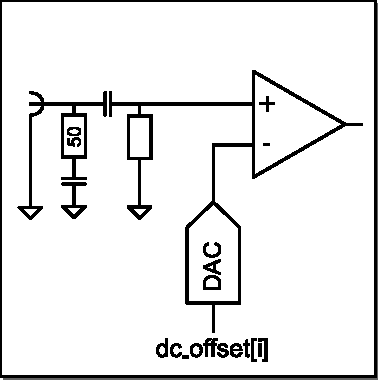
\includegraphics[width=0.3\textwidth]{xhptdc/figures/InputCircuit.pdf}
			}{
				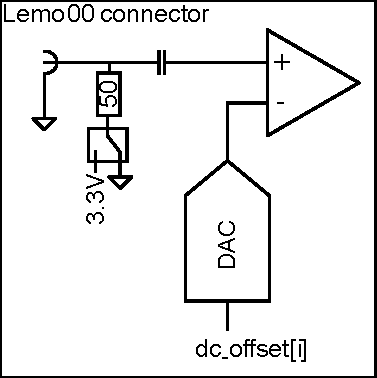
\includegraphics[width=0.3\textwidth]{figures/InputCircuit.pdf}
			}
			\caption{Input circuit for each of the input channels. \label{fig:dcoffset1}}
		\end{center} 
	\end{figure}
%%			\begin{figure}
%%				\begin{center}
%%					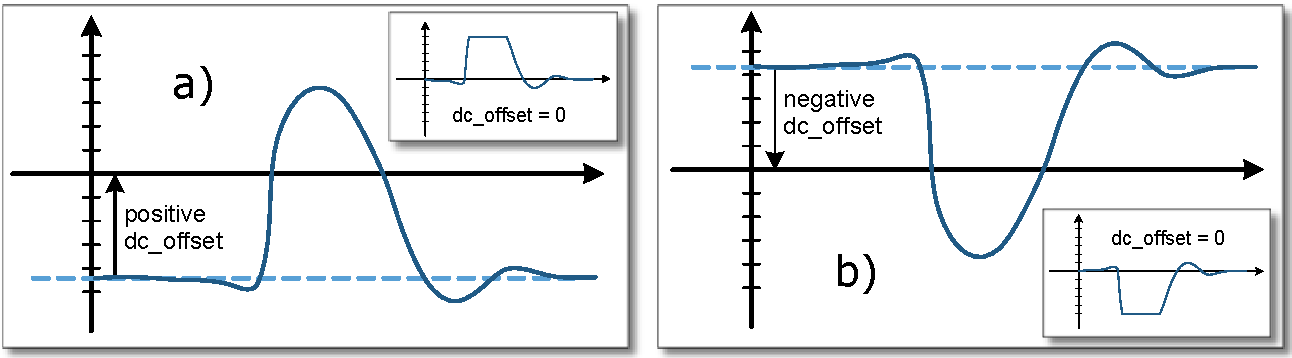
\includegraphics[width=\textwidth]{figures/dc_offset.pdf}
%%%					\caption{\textit{dc\tu offset} is used to shift the signal on each input channel such that the noise margin relative to the switching threshold is maximized.
%%					Insets of figure a) and b) show the base line of the signal with $\mathrm{\textit{dc\tu offset}}~=~0$ close to the switching threshold of the input buffer. Figure a) shows the positive pulse with $\mathrm{\textit{dc\tu offset}}~>~0$ and figure b) shows the negative pulse with $\mathrm{\textit{dc\tu offset}}~<~0$.\label{fig:dcoffset2}}
%%				\end{center}
%%			\end{figure}

	\ttvar{\prefix trigger}{trigger[\PREFIX TRIGGER\tu COUNT]}\\
	Configures the polarity of the external trigger sources.
	These are used as inputs for the TiGer blocks and as inputs to the time measurement unit.\par

	\ttvar{\prefix tiger\tu block}{tiger\tu block[\PREFIX TIGER\tu COUNT]}\\
	Configuration of the timing generators (TiGer).

	\ifxHPTDC{
		\ttvar{\prefix tiger\tu block}{gating\tu block[\PREFIX GATE\tu COUNT]}\\
		Configuration of the gating blocks.	
	}{} % only for xHPTDC8

	\ttvar{\prefix channel}{channel[\PREFIX CHANNEL\tu COUNT]}\\
		Configure the TDC channels.

	\ifxHPTDC{
		\cronvar{crono\tu bool\tu t}{skip\tu alignment}\\
		If set,  the phase of the two TDC chips is not realigned when capturing is restartet.

		\cronvar{crono\tu bool\tu t}{alignment\tu source}\\
		Define a signal source that is used for phase alignment. Should usually be left unchanged.
		\begin{tabular}{ll}
			\ttdef{ALIGN\tu TIGER} & 0\\
			\ttdef{ALIGN\tu PIN} & 1\\
			\ttdef{ALIGN\tu RESERVED} & 2\\
		\end{tabular}\par
		
	}{
		\ttvar{\prefix low-res\tu channel}{low-res\tu channel[\PREFIX LOWRES\tu CHANNEL\tu COUNT]}\\
		\itett{
			Not applicable for \deviceName. 
		}{
			Only applicable to the xTDC4-Sciex. Configures the additional digital low-res inputs.
		}\par
		\autotrigger
	
	}

	

%%%%%%%%% trigger
	\subsection{Structure \prefix trigger}
	\label{structtrigger}
	For each input this structure determines wheter rising or falling edges on the inputs create trigger events for the TiGer \ifxHPTDC{and gating}{} blocks.

	\cronvar{crono\tu bool\tu t}{falling}\\
	\cronvar{crono\tu bool\tu t}{rising}\\
	Select for which edges a trigger event is created inside the FPGA.
	\txh{
		Set the corresponding flag for one of the edges or both edges then using the input with a TiGer.
	}{
		The \deviceName can output measurements with a reduced bin size of $5/6~ns = 833,\overline{3}~ps$ for one or both edges of input signals. 
		See section \ref{difficulthits} for more information on hits with varying resolution.
		Use \textsf{xtdc4\tu channel.rising} on page \pageref{structchannel} to select which edge is measured with full resolution.
		The edge that is selected for full resolution measurement must also be enabled for low resolution measurement.
	}{
		While the TDC can only measure either rising or falling edges, the gating blocks and the TiGer are more flexibel. 
		Set the corresponding flag for one of the edges or both edges when using the input with a TiGer or gating block.
	}\par

%%%%% tiger_block			

	\subsection{Structure \prefix tiger\tu block\label{cp:tigerblock}}
	See section \ref{cp:tiger} for additional information.
	\ifxHPTDC{
		\cronvar{int}{mode}\\*
		Enables the desired mode of operation for the tiger. \\*
		\begin{tabular}{lrl}
			\ttdef{TIGER \tu OFF} & 0 & No operation \\
			\ttdef{TIGER \tu OUTPUT} & 1 & Output is driven with 2V amplitude. \\*
										&   &There must be no input connected \\
			\ttdef{TIGER \tu BIDI} & 2 & Output is driven with 1V amplitude. \\*
									&   & Pulse rate should be low. \\*
			\ttdef{TIGER \tu BIPOLAR} & 3 & Output is driven with 1~V bidirectional pulses.\\*
									&   & $start = stop -1$\\*
		\end{tabular}
		The gating blocks are only used internally and produce no pulses accessible to the user.		
		Gating blocks interpret any value that is not 0 as as enable.\\*
		\begin{tabular}{lrl}
			\ttdef{GATE \tu OFF} & 0 & No gating, alle hits are captured. \\*
			\ttdef{GATE \tu ON} & 1 & No hits are captured while the gate is active.\\*
		\end{tabular}
	
	}{
		\cronvar{crono\tu bool\tu t}{enable}\\
		Activates the timing generator (TiGer).\par
	}

	\cronvar{crono\tu bool\tu t}{negate}\\
	Inverts output polarity. Default is set to false.
	\ifxHPTDC{For gating blocks, a value of false blocks inputs between start and stop, a value of true blocks outputs outside that interval.
	The TiGer creates a high pulse from \textsf{start} to \textsf{stop} unless negated.}{}\par

	\cronvar{crono\tu bool\tu t}{retrigger}\\
	Enables retrigger setting.\\
	If enabled the timer is reset to the value of the \textsf{start} parameter, whenever the input signal is set while waiting to reach the \textsf{stop} time.\par

	\cronvar{crono\tu bool\tu t}{extend}\\
	Not implemented.

	\ifxHPTDC{}{
		\cronvar{crono\tu bool\tu t}{enable\tu lemo\tu output}\\
		Enables the LEMO output. Drive the TiGer Signal to the corresponding Lemo connector as an output. 
		This is DC coupled, so make sure that you do not any devices connected as inputs.
		Pulses created by the TiGer are visible at the \deviceName inputs and can be measured again to get the exact timing.  
	}

	\cronvar{int}{start}\\
	\cronvar{int}{stop}\\
	\itett{
		In multiples of $4~ns$.
	}{
		In multiples of $20~ns/3 = 6,\overline{6}~ns$
	}
	The time during which the TiGer output is set, relative to the trigger input. The parameters \textsf{start} and \textsf{stop} must fulfill the following conditions:
	\[ 0 <= start <= stop <= 2^{16}-1 \]
	If retriggering is enabled, the timer is reset to the value of the start parameter whenever the input signal is set while waiting for the stop time. \par
	

	\cronvar{int}{sources}\\
	A bit mask with a bit set for all trigger sources that can trigger this TiGer block. 
	Default is \textsf{\PREFIX TRIGGER\tu SOURCE\tu \ifxHPTDC{A}{S}}.\par

	\begin{tabular}{lc}
			\ttdef{TRIGGER\tu SOURCE\tu NONE} & 0x00000000\\
		\ifxHPTDC{
			\ttdef{TRIGGER\tu SOURCE\tu A} & 0x00000001\\
			\ttdef{TRIGGER\tu SOURCE\tu B} & 0x00000002\\
			\ttdef{TRIGGER\tu SOURCE\tu C} & 0x00000004\\
			\ttdef{TRIGGER\tu SOURCE\tu D} & 0x00000008\\
			\ttdef{TRIGGER\tu SOURCE\tu E} & 0x00000010\\
			\ttdef{TRIGGER\tu SOURCE\tu F} & 0x00000020\\
			\ttdef{TRIGGER\tu SOURCE\tu G} & 0x00000040\\
			\ttdef{TRIGGER\tu SOURCE\tu H} & 0x00000080\\
			\ttdef{TRIGGER\tu SOURCE\tu TDC1\tu SYNC} & 0x00000100\\
			\ttdef{TRIGGER\tu SOURCE\tu TDC2\tu SYNC} & 0x00000200\\
			\ttdef{TRIGGER\tu SOURCE\tu TDC\tu EXT\tu SYNC} & 0x00000400\\
			\ttdef{TRIGGER\tu SOURCE\tu ADC1\tu CONV} & 0x00000800\\
			\ttdef{TRIGGER\tu SOURCE\tu ADC2\tu CONV} & 0x00001000\\
			\ttdef{TRIGGER\tu SOURCE\tu AUTO} & 0x00004000\\
			\ttdef{TRIGGER\tu SOURCE\tu ONE}  & 0x00008000	
		}{
				\ttdef{TRIGGER\tu SOURCE\tu S} & 0x00000001\\
				\ttdef{TRIGGER\tu SOURCE\tu A} & 0x00000002\\
				\ttdef{TRIGGER\tu SOURCE\tu B} & 0x00000004\\
				\ttdef{TRIGGER\tu SOURCE\tu C} & 0x00000008\\
				\ttdef{TRIGGER\tu SOURCE\tu D} & 0x00000010\\
				\ttdef{TRIGGER\tu SOURCE\tu AUTO} & 0x00004000\\
				\ttdef{TRIGGER\tu SOURCE\tu ONE} & 0x00008000
		}
	\end{tabular} 

%%%%%%%%%%%%%%%%%%%%%%%% channel

	\subsection{Structure \prefix channel}
		\label{structchannel}
		Contains TDC channel settings.\par

		\cronvar{crono\tu bool\tu t}{enable\ifxHPTDC{}{d}}\\
		Enable TDC channel.\par

		\cronvar{crono\tu bool\tu t}{rising}\\
		\txh{
			Not applicable for \deviceName.
		}{
			Select which edge of the signal is used for full resolution measurements. 
			\textsf{xtdc4\tu trigger.rising} and \textsf{xtdc4\tu trigger.falling} described on page \pageref{structtrigger} are used 
			to select which edges are recorded for low resolution measurement. 
			The edge that is selected for full resolution measurement must also be enabled for low resolution measurement.
			See section \ref{difficulthits} for more information on hits with varying resolution.
		}{
			Select which edge of the signal is measured by the TDC. 
			The TiGer and gating blocks use a separate configuration that allows to use both edges simultaneously on each input. See section \ref{structtrigger}
		}\par

		\txh{}{ %only for xTDC4
			\cronvar{crono\tu bool\tu t}{cc\tu enable}\\
			Enable carry chain TDC. This is set to \emph{true} by default and should be left unchanged. \par

			\cronvar{crono\tu bool\tu t}{cc\tu same\tu edge}\\
			Sets whether the carry chain TDC records the same or opposite edge as the TDC chip. 
			If the same edge is selected, that carry chain TDC acts  as a backup if the chip misses hits due to FIFO overflows or short input pulses.
			If opposite edges are selected, both edges of a pulse can be measured with reasonable resolution. See section \ref{difficulthits} for more information.\par

			\cronvar{crono\tu bool\tu t}{ths788\tu disable}\\
			Disable full resolution timestamps. This is set to \emph{false} by default and should be left unchanged.\par
		}{}

		\ifxHPTDC{}{
			\cronvar{int}{start}\\
			\cronvar{int}{stop}\\
			Veto function for grouping of hits into packets in multiples of the binsize. Only hits between start and stop are read out.
			The parameters must adhere to the following relations:
			\[
				0 <= start <= stop < 2^{ \itett{31}{30}}
			\]
		}

%%%%%%%%%%%%%%%%%%%%% grouping, only fpr xHPTDC8

\ifxHPTDC{
	\subsection{Structure \prefix grouping\tu configuration}	
	\label{structgrouping}
	This structure configures the behaviour of the grouping functionality. See section \ref{grouping}.
	Grouping is enabled with the \textsf{tdc\tu mode} paramter defined in the top level of the config structure.

	In this structure intervals are always provided in picoseconds, independently of the bin size of the TDC.

	\cronvar{bool}{enable}
	Enable grouping. Defaults to \textsf{false}.

	\cronvar{int}{trigger\tu channel}\\
	Channel number that is used to trigger the creation of a group.\par

	\cronvar{int}{zero\tu channel}\\
	Optionally a different channel can be used to calculate the relative timestamps in a group. 
	This is disabled per default by setting this paramteer to $-1$.\par
	
	\cronvar{\tu\tu int64}{zero\tu channel\tu offset}\\
	This offset in picoseconds is added to relative timestamps within a group.\par

	\cronvar{\tu\tu int64}{range\tu start}\\
	\cronvar{\tu\tu int64}{range\tu stop}\\
	Values in the interval from \textsf{range\tu start} to \textsf{range\tu stop} are included in the group. 
	Either or both values can be negative to create common-stop behaviour. 
	\[
		-2^{63} \le range\_start \le range\_stop < 2^{63} 
	\]\par

	\cronvar{\tu\tu int64}{trigger\tu deadtime}\\
	After a trigger was detected additional triggers will be suppressed for this interval. Must not be negative.\par

	\cronvar{crono\tu bool\tu t}{require\tu windows\tu hit}\\
	If set a group is only created if there is at least one hit in the window defined by \textsf{window\tu start} and \textsf{window\tu stop}.\par

	\cronvar{\tu\tu int64}{window\tu start}\\
	\cronvar{\tu\tu int64}{window\tu stop}\\
	\[
		-2^{63} \le window\_ start \le window\_ stop < 2^{63} 
	\]\par

	\cronvar{int}{veto\tu mode}\\
	A window defined by \textsf{veto\tu start} and \textsf{veto\tu stop} can be used to suppress hits. 
	The functionality is very similar to the gating blocks but is defined in software. 
	While gating blocks can only work locally on the information available within each board the veto function is applied globally accross all boards.
	This feature can not be used to improve FIFO usage or PCIe bandwidth usage. 
	 \\*
	Either data inside or outside the veto window can be suppressed.\\*
	\begin{tabular}{lc}
		\ttdef{VETO\tu OFF}     & 0 \\
		\ttdef{VETO\tu INSIDE}  & 1 \\
		\ttdef{VETO\tu OUTSIDE} & 2 \\
	\end{tabular}\par

	\cronvar{\tu\tu int64}{veto\tu start}\\
	\cronvar{\tu\tu int64}{veto\tu stop}\\
	\[
		-2^{63} \le veto\_ start \le veto\_ stop < 2^{63} 
	\]\par

	\cronvar{crono\tu bool\tu t}{veto\tu relative\tu zero}\\
	If set, the veto window is defined relative to the zero channel. Otherwise the window is defined relative to the trigger.\par 

	\cronvar{crono\tu bool\tu t}{overlap}\\
	Unsupported, must remain \textsf{false}.

}{}



	
  
		  
	\chapter{Run Time Control\label{cp:readout}}  % and packet format
		\ifxHPTDC{
				%%%%%%%%%%%%%%%%% run time control
	\section{Controlling the State of the Driver}
	Once the devices are configured the following functions can be used to control the behaviour of the devices. 
	All of these functions return quickly with very little overhead, but they are not guaranteed to be thread safe.

		\ttvar{int}{start\tu capture(}\device)\\
		Start data acquisition.\par

		\ttvar{int}{pause\tu capture(}\device)\\
		Pause a started data acquisition. 
		Pause and continue have less overhead than start and stop but don't allow for a configuration change.\par

		\ttvar{int}{continue\tu capture(}\device)\\
		Call this to resume data acquisition after a call to \textsf{\prefix pause\tu capture()}.
		Pause and continue have less overhead than start and stop but don't allow for a configuration change.\par

		\ttvar{int}{stop\tu capture(}\device)\\
		Stop data acquisition.\par

		\ttvar{int}{start\tu tiger(}\device, \cronvar{int}{index})\\
		\ttvar{int}{stop\tu tiger(}\device, \cronvar{int}{index})\\
		Start and stop the timing generator of an individual board. 
		This can be done independently of the state of the data acquisition.\par	


\section{Readout}

\ttvar{int}{read\tu hits(}\device,  \cronvar{TDCHit}{*hit\tu buf,} \cronvar{size\tu t}{size} )\\
Read a multitude of hits into a buffer provided by the user. Returns the number of read hits.\\
If grouping is enabled a single group is read. 
If the group is to large for the buffer the remaining hits of the group are discarded.\\*
If grouping is disabled, all availabe data is read up to the size of the buffer. \\
The method always returns immediately. If no hits are read it of is beneficial to call \textsf{sleep()} 
or yield the CPU to another process instead of trying again immediately.\\
Make sure to set \textsf{size} to the number of elemenst that fit into the buffer.\\*

This function is not thread safe. 
If you want to process the read data in multiple threads the data needs to be copied to a seperate buffer for each thread.






		}{
			% NOTE: xHPTDC has a seperate file describing the readout

%%%%%%%%%%%%%%%%% run time control
\section{Run Time Control}
	\ttvar{int}{start\tu capture(}\device)\\
	Start data acquisition.\par

	\ttvar{int}{pause\tu capture(}\device)\\
	Pause a started data acquisition. 
	Pause and continue have less overhead than start and stop but don't allow for a configuration change.\par

	\ttvar{int}{continue\tu capture(}\device)\\
	Call this to resume data acquisition after a call to \textsf{\prefix pause\tu capture()}.
	Pause and continue have less overhead than start and stop but don't allow for a configuration change.\par

	\ttvar{int}{stop\tu capture(}\device)\\
	Stop data acquisition.\par

	\ttvar{int}{start\tu tiger(}\device)\\
	Start timing generator. This can be done independently of the state of the data acquisition.\par

	\ttvar{int}{stop\tu tiger(}\device)\\
	Stop timing generator. This can be done independently of the state of the data acquisition.\par

%%%%%% readout
\section{Readout}
	\ttvar{int}{acknowledge(}\device, \cronvar{crono\tu packet}{*packet)}\\
	Acknowledges the processing of the last read block. This is only necessary if \textsf{\prefix read()} is not called with 
	\textsf{in.acknowledge\tu last\tu read} set.\\
	This feature allows to either free up partial DMA space early if there will be no call to \textsf{\prefix read()} anytime soon. 
	It also allows to keep data over multiple calls to \textsf{\prefix read()} to avoid unnecessary copying of data. \par

	\ttvar{int}{read(}\device \cronvar{\prefix read\tu in}{*in,} \\ \cronvar{\prefix read\tu out}{*out)}\\
	Return a pointer to an array of captured data in \textsf{read\tu out}. 
	The result can contain any number of packets of type \textsf{\prefix packet}.
	\textsf{read\tu in} provides parameters to the driver. 
	A call to this method automatically allows the driver to reuse the memory returned in the previous call if \textsf{read\tu in.acknowledge\tu last\tu read} is set.\\
	Returns an error code as defined in the structure \textsf{\prefix read\tu out}.

	\subsection{Input Structure \prefix read\tu in}

		\ttvar{\prefix bool\tu t}{acknowledge\tu last\tu read}\\
		If set \textsf{\prefix read()} automatically acknowledges packets from the last read. 
		Otherwise \textsf{\prefix acknowledge()} needs to be called explicitely be the user. 

	\subsection{Input Structure \prefix read\tu out}
		\cronvar{crono\tu packet}{*first\tu packet}\\
		Pointer to the first packet that was captureed by the call of \textsf{\prefix read()}.\par

		\cronvar{crono\tu packet}{*last\tu packet}\\
		Address of header of the last packet in the buffer.\par

		\cronvar{int}{error\tu code}\\
		Assignments of the error codes.\par
		\begin{tabular}{lc}
			\crondef{CRONO\tu READ\tu OK} & 0\\
			\crondef{CRONO\tu READ\tu NO\tu DATA} & 1\\
			\crondef{CRONO\tu READ\tu INTERNAL\tu ERROR} & 2\\
			\crondef{CRONO\tu READ\tu TIMEOUT} & 3\par
		\end{tabular}\par

		\cronvar{const char}{*error\tu message}
		The last error in human readable form, possibly with additional information on the error.

	
		} 

	\chapter{Output Data Format\label{cp:packetformat}} 
		\ifxHPTDC{
			For each measured edge the \deviceName\ creates a 12 byte data structure TDCHit that contains a 64 bit timestamp in picoseconds and three fields with additional information. 

\section{Structure TDCHit}
\label{TDCHit}
\cronvar{long long}{time}\\
The time stamp of the hit in picoseconds. 

If grouping is disabled the timestamps are continuously counting up from the call to \textsf{start\tu capture()}.

If grouping is enabled the timestamps are relative to the trigger or the separate zero reference of the group. 
The first of a group has channel number 255 and provides the absolute time of the group. 
The absolute time of each of the hits can be obtained by adding this value to each of the relative timestamps.

\cronvar{unsigned char}{channel}\\
For the first board in the system this is 0 to 7 for the TDC channels A to H. 8 or 9 for ADC data. Data from channels 8 and 9 should usually be treated as data from the same channel. 
For the other boards the channel number is incremented by $board\_id \cdot 10$.
In grouping mode the first hit of each group has channel number 255 and contains the absolute time of the group.

\cronvar{unsigned char}{type}\\
Additional information on the type of hit recorded. See section \ref{hittypes}.

\cronvar{unsigned short}{bin}\\
For ADC hits this contains the sampled voltage. For TDC hits the content is undefined.

\newpage
\subsection{TDCHit Types \label{hittypes}}
\newcommand{\HTYPE}{\PREFIX TDCHIT\tu TYPE\tu}

\paragraph*{Type information for TDC measurements}
If the hit is a TDC measurement on channels A to H the following flags are defined for the \textsf{type} field of the TDCHit structure:\\*
\begin{tabular}{lc}
    \crondef{\HTYPE RISING} & 0x01\\
    \indent Rising edge &\\
    \crondef{\HTYPE ERROR}  & 0x02\\
    \indent any type of error& \\
    \crondef{\HTYPE ERROR\tu TIMESTAMP\tu LOST}  & 0x04\\
    \indent Hits missing due to L1 FIFO overflow&\\
    \crondef{\HTYPE ERROR\tu ROLLOVER\tu LOST}  & 0x08\\
    \indent Invalid timestamp due to internal error&\\
    \crondef{\HTYPE ERROR\tu PACKET\tu LOST}  & 0x10\\
    \indent Hits missing due to a lost DMA packet&\\
    \crondef{\HTYPE ERROR\tu SHORTENED}  & 0x20\\
    \indent Hits missing due to a shortened DMA packet&\\
    \crondef{\HTYPE ERROR\tu DMA\tu FIFO\tu FULL}  & 0x40\\
    \indent Hits missing due to L2 FIFO overflow&\\
    \crondef{\HTYPE ERROR\tu HOST\tu BUFFER\tu FULL}  & 0x80\\
    \indent Hits missing due to host buffer overflow &\\
\end{tabular}

If hits are missing the error flag is set on the next hit from the same board that is read out.

\paragraph*{Type information for ADC measurements}
If the hit is an ADC measurement on channels 8 or 9 the following flags are defined for the \textsf{type} field of the TDCHit structure:\\*
\begin{tabular}{lc}
    \crondef{\HTYPE ADC\tu INTERNAL} & 0x01\\
    \indent ADC measurement triggered by TiGer &\\
    \crondef{\HTYPE ADC\tu ERROR}  & 0x02\\
    \indent any type of error& \\
    \crondef{\HTYPE ADC\tu ERROR\tu INVALID\tu TRIGGER}  & 0x08\\
    \indent TRG input violated timing requirements. Data may be corrupted&\\
    \crondef{\HTYPE ADC\tu ERROR\tu DATA\tu LOST}  & 0x10\\
    \indent ADC measurement missing due to overflow of any buffer&\\
\end{tabular}

If hits are missing the error flag is set on the next hit from the same board that is read out.


 
		}{
			


\section{Output Structure crono\tu packet}

	\cronvar{unsigned char}{channel}\\
	Unused, always 0.\par

	\cronvar{unsigned char}{card}\\
	Identifies the source card in case there are multiple boards present. Defaults to 0 if no value is assigned to the parameter \textsf{board\tu id} in Structure \textsf{ndigo\tu init\tu parameters}.\par

	\cronvar{unsigned char}{type}\\
	The data stream consists of 32-bit unsigned data as signified by a value of 6.\par

	\cronvar{unsigned char}{flags}\\
	\indent\ttdef{ PACKET\tu FLAG\tu ODD\tu HITS} 1\\
	\indent The last data word in the data array consists of one timestamp only which is located in the lower 32 bits of the 64-bit data word (little endian).\par
	\indent\ttdef{ PACKET\tu FLAG\tu SLOW\tu SYNC} 2\\
	\indent Start pulse distance is larger than the extended timestamp counter range.\par
	\indent\ttdef{ PACKET\tu FLAG\tu START\tu MISSED} 4\\
	\indent The trigger unit has discarded packets due to a full FIFO.\par
	\indent\ttdef{ PACKET\tu FLAG\tu SHORTENED} 8\\
	\indent The trigger unit has shortened the current packet due to full FIFO.\par
	\indent\ttdef{ PACKET\tu FLAG\tu DMA\tu FIFO\tu FULL} 16\\
	\indent The internal DMA FIFO was full. Might or might not result in dropped packets.\par
	\indent\ttdef{ PACKET\tu FLAG\tu HOST\tu BUFFER\tu FULL} 32\\
	\indent The host buffer was full. Might or might not result in dropped packets.\par

	\cronvar{unsigned int}{length}\\
	Number of 64-bit elements (each containing up to 2 TDC hits) in the data array.\par

	\cronvar{unsigned \tu\tu int64}{timestamp}\\
	Coarse timestamp of the start pulse. Values are given in multiples of \itett{$500$~ps}{$5/3=1.\overline{6}$~ns}.\par

	\cronvar{unsigned \tu\tu int64}{data[1]}\\
	TDC hits. the user can cast the array to uint32* to directly operate on the TDC hits.

	\noindent
	\begin{small}
	\begin{tabular}{|c||p{9cm}|p{1,5cm}|p{1,5cm}|}
		\hline
		bits & 31~ ~ ~ ~ ~ ~ ~ ~ ~ ~ ~ ~ ~ ~ ~ ~ ~ to ~ ~ ~ ~ ~ ~ ~ ~ ~ ~ ~ ~ ~ ~ ~ ~ ~ 8 & 7~ ~ to ~ ~ 4 & 3~ ~ to ~ ~ 0\\\hline
		content & TDC DATA & FLAGS & CHN \\\hline
	\end{tabular}
	\end{small}

	The timestamp of the hit is stored in bits 31 down to 8 in multiples of 
	\itett{500~ps. For the -1G Variant bit 8 is always 0.}{
		$5/(3*128) = 13.0208\overline{3}$~ps
	}\\
	
	\label{flags}
	Bits 7 down to 4 are hit flags:\par
	\itett{
		Bit 7: Always 0.\par
		Bit 6: Always 1.\par
	} {
		Bit 7, 6: Resolution of this measurement. \ifxHPTDC{}{See section \ref{difficulthits}}.\\
		\noindent
		\begin{small}
		\begin{tabular}{|c|c||l|}
			\hline
			bit 7 & bit 6 & Measurement Type \\\hline\hline
			0 & 0 &  Normal full resolution measurement.\\\hline
			0 & 1 &  Measurement performed with carry chain TDC at about 150~ps resolution.\\\hline
			1 & 0 &  Full resolution measurement that might in the wrong place in the data stream.\\\hline
			1 & 1 &  Measurement with only $5/6~ns = 833.\overline{3}~ps$ resolution. \\\hline
		\end{tabular}
		\end{small}
		
	}
	Bit 5: Rollover. The time since start pulse exceeded the \itett{23}{24}-bit range that can be ecnoded in a data word. This word does not encode a measurement. 
	Instead the readout software should increment a rollover counter that can be used as the upper bits of consecutive time stamps.  
	The counters should be reset for each packet.
	The total offset of a hit in picoseconds can be computed by
	\[	\Delta T_{hit} = \mathrm{(\#\ rollovers \cdot 2^{\itett{23}{24}} + TDC\_ DATA_{hit}) \cdot \itett{timetagger4}{xtdc4}\_param\_info.binsize} \]
	\indent
	Bit 4: Set if this word encodes a rising edge. Otherwise, this word belongs to a falling edge.
	The channel number is given in the lowest nibble of the data word. A value of 0 corresponds to channel A, a value of 3 to channel D.\par
 
		}  
 
	\chapter{C Example}  
		% SVN Info:
% $Date: 2021-01-31 20:06:56 +0100 (So, 31 Jan 2021) $
% $Rev: 1040 $
% $Author: kolja $

	The following C++ source code shows how to initializes a \deviceName\ board, configure it and loop over incoming packets.	

	If you are reading this documentation in portable document format, the source code of the C example is also embedded as an
	\txh{
		\textattachfile[color=cronlightgreen, description={Example Source Code}]{"timetagger/example.cpp"}{attachment}
		to the file. You can open it in an external viewer or save it to disk by clicking on it.
		\lstinputlisting{timetagger/example.cpp}
	}{
		\textattachfile[color=cronlightgreen, description={Example Source Code}]{xtdc/example.cpp}{attachment}
		to the file. You can open it in an external viewer or save it to disk by clicking on it.
		\lstinputlisting{xtdc/example.cpp}
	}{	
		\textattachfile[color=cronlightgreen, description={Example Source Code}]{xhptdc/example.cpp}{attachment}
		to the file. You can open it in an external viewer or save it to disk by clicking on it.

		The example code is managed as open source on GitHub at 
		\href{https://github.com/cronologic-de/xhptdc8_babel/tree/main/ug_example}{https://github.com/cronologic-de/xhptdc8\tu babel}. 
		The repository contains a complete project for Microsoft Visual Studio that you can use to compile the example.
		Examples for more programming languages such as Golang, Rust, Python and LabView will be added to the repository over time.

		At the time this document is written, the following source code can be found in the repository:
		\begin{itemize}
			\item \href{https://github.com/cronologic-de/xhptdc8_babel/tree/main/dummy}{dummy library} to be able to develop code for the \deviceName\ without a physical board beeing present
			\item \href{https://github.com/cronologic-de/xhptdc8_babel/tree/main/util}{utility library} to configure the device from YAML strings or YAML files 
			\item command line info tool to list information about all \deviceName\ boards in the system. This tool is written in Go.
		\end{itemize}

		\lstinputlisting{xhptdc/example.cpp}
	}
	% there were problems with underscores in file names so we removed them



	\chapter{Technical Data}    
		\ttinput{Tech.tex} 
		% SVN Info:
% $Date: 2021-01-29 22:28:41 +0100 (Fr, 29 Jan 2021) $
% $Rev: 1039 $
% $Author: kolja $
\section{Electrical Characteristics}

	\subsection{Power Supply}

		\noindent
		\begin{tabularx}{\textwidth}{|c|X|c|c|c|c|}
			\hline
			Symbol & Parameter & Min & Typical & Max & Units\\
			\hline\hline
			P & Total power consumption &&& 25& W\\
			\hline
			I & PCIe 3,3V rail input current &&&4& mA\\
			\hline
			VCC & PCIe 3,3V rail power supply voltage &3,1&3,3&3,5& V\\
			\hline
			I & PCIe 12V rail input current &&&2,1& A\\
			\hline
			VCC & PCIe 12V rail power supply voltage &11,1&12&12,9& V\\
			\hline
			I & PCIe 3,3VAux rail input current &&0&& A\\
			\hline
			VCC & PCIe 3,3VAux rail power supply voltage &&3,3&& V\\
			\hline
		\end{tabularx}

	\subsection{TDC Inputs}

		The \deviceName's inputs are single-ended AC-coupled with 50$\Omega$ DC termination.

		\noindent
		\begin{tabularx}{\textwidth}{|c|X|c|c|c|c|}
			\hline
			Symbol & Parameter & Min & Typical & Max & Units\\
			\hline\hline
			V\subscript{Base} & Input Baseline & 0 & & 5 & V\\
			\hline
			V\subscript{Threshold} & Trigger Level & V\subscript{Base} - 1.32 & & V\subscript{Base} + 1.18 & V\\
			\hline
			t\subscript{Pulse} & Pulse Length & 2 & 5 & 200 & ns\\
			\hline
			t\subscript{Rise} & Pulse Edge 20\% to 80\%  &  &  & 10 & ns\\
			\hline
			t\subscript{Fall} & Pulse Edge 80\% to 20\%  &  &  & 10 & ns\\
			\hline
			Z\subscript{P} & Input Impedance && 50 && $\Omega$\\
			\hline
			I\subscript{Term} & Termination Current & -50 & -20 & 50 & mA\\
			\hline
		\end{tabularx}

	All inputs are AC coupled. The inputs have very high input bandwidth requirements and therefore there are no circuits that provide over voltage protection for these signals. 
	Any voltage on the inputs above 5V or below -5V relative to the voltage of the slot cover can result in permanent damage to the board.
	
	\ifxHPTDC{
		All digital inputs can output AC coupled pulses from the TiGer. 
		Special care should be taken not to enable the TiGer output when sensitive equipment is connected that could be damaged by the pulses. 
	}{
		Make sure not to drive the inputs when the connector is configured as a TiGer output. 
	}
	See Section \ref{cp:tiger}. 
%%%%%%%%%%% ADC input
	\ifxHPTDC{
	\newpage
	\subsection{ADC Inputs}
	The ADC input is DC coupled to a differential termination voltage of 400~mV. 
	This means that the actual voltage seen by the ADC will depend on the output impedance of the source that is driving the input.\\*
	\noindent
		\begin{tabularx}{\textwidth}{|c|X|c|c|c|c|}
			\hline
			Symbol & Parameter & Min & Typical & Max & Units\\
			\hline\hline
			V\subscript{in} & Input voltage & -2.0 &  & 2.5 & V \\
			\hline 
			V\subscript{term} & Termination voltage & & 0.4 & & V \\
			\hline 
			Z\subscript{in} & Input Impedance & & 50  & & $\Omega$ \\
			\hline
		\end{tabularx}

%%%%%%%%%%% clock input		
	\subsection{Clock input J2}
	The ADC input is DC coupled to a differential termination voltage of 400~mV. 
	This means that the actual voltage seen by the ADC will depend on the output impedance of the source that is driving the input.\\*
	\noindent
		\begin{tabularx}{\textwidth}{|c|X|c|c|c|c|}
			\hline
			Symbol & Parameter & Min & Typical & Max & Units\\
			\hline\hline
			V\subscript{p-p} & Peak to Peak voltage & 1 &  & 3.3 & V \\
			\hline 
			V\subscript{cm} & Common mode voltage voltage &-3 & 0 & 3 & V \\
			\hline 
			V\subscript{tck} & Clock termination voltage & & 0 &  & V \\
			\hline 
			Z\subscript{in} & Input Impedance & & 50  & & $\Omega$ \\
			\hline 
			D\subscript{J2} & Duty cycle & 45 & 50 & 55 & \% \\
			 \hline 
			 f\subscript{J2}& Frequency &  & 10 &  & MHz \\
			\hline
		\end{tabularx}
}{}

\newpage
\section{Information Required by DIN EN 61010-1}
\subsection{Manufacturer\label{cp:manu}}

The \deviceName\ is a product of:\

\begin{quote}
	cronologic GmbH \& Co. KG\\
	Jahnstra\ss{}e 49\\
	60318 Frankfurt\par
	Germany
	\noindent HRA 42869 beim Amtsgericht Frankfurt/M\par
	\noindent VAT-ID: DE235184378
	\noindent PCI Vendor ID: 0x1A13
\end{quote}

\subsection{Intended Use and System Integration}

	The devices are not ready to use as delivered by cronologic. It requires the development of specialized software to fulfill the application of the end user. The device is provided to system integrators to be built into measurement systems that are distributed to end users. These systems usually consist of the \deviceName, a main board, a case, application software and possible additional electronics to attach the system to some type of detector. They might also be integrated with the detector.\par

	The \deviceName\ is designed to comply with DIN EN 61326-1 when operated on a PCIe compliant main board housed in a properly shielded enclosure. 
	When operated in a closed standard compliant enclosure the device does not pose any hazards as defined by EN 61010-1.\par

	Radiated emissions, noise immunity and safety highly depend on the quality of the enclosure. 
	It is the responsibility of the system integrator to ensure that the assembled system is compliant to applicable standards of the country that the system is operated in, especially with regards to user safety and electromagnetic interference. \par
	 
	When handling the board, adequate measures must be taken to protect the circuits against electrostatic discharge (ESD). All power supplied to the system must be turned off before installing the board.

	\subsection{Environmental Conditions for Storage}

	The board shall be stored between operation under the following conditions:

	\noindent
	\begin{tabularx}{\textwidth}{|c|X|c|c|c|c|}
		\hline
		Symbol & Parameter & Min & Typical & Max & Units\\
		\hline\hline
		T & ambient temperature & -30 && 60 & $^{\circ}$C\\
		\hline
		RH & relative humidity at 31$^{\circ}$C noncondensing & 10 && 70 & \%\\
		\hline
	\end{tabularx}


\subsection{Environmental Conditions for Operation}

	The board is designed to be operated under the following conditions:

	\noindent
	\begin{tabularx}{\textwidth}{|c|X|c|c|c|c|}
		\hline
		Symbol & Parameter & Min & Typical & Max & Units\\
		\hline\hline
		T & ambient temperature & 5 && 40 & $^{\circ}$C\\
		\hline
		RH & relative humidity at 31$^{\circ}$C & 20 && 75 & \%\\
		\hline
	\end{tabularx}

	WARNING: Do not connect any DC coupled inputs to a channel while the TiGer of that channel is configured as an output (see Section \ref{cp:tiger}).
	Doing so could do permanent damage to the \deviceName\ and the external hardware.

\subsection{Cooling}

	The \deviceName\ in its base configuration has passive cooling that requires a certain amount of air flow. 
	If the case design can't provide enough air flow to the board, a slot cooler like Zalman ZM-SC100 can be placed next to the board. 
	Active cooling is also available as an option for the board.


\subsection{Recycling}

	cronologic is registered with the ``Stiftung Elektro-Altger\"a{}te Register'' as a manufacturer of electronic systems with Registration ID DE 77895909.\par
	The \deviceName\ belongs to category 6, ``Kleine Geräte der Informations- und Telekommunikationstechnik für die ausschließliche Nutzung in anderen als privaten Haushalten''. 
	Devices sold before 2018 belong to category 9, ``\"U{}berwachungs und Kontrollinstrumente f\"u{}r aus\-schlie\ss lich gewerbliche Nutzung''. 
	
	The last owner of a \deviceName\ must recycle it, treat the board in compliance with \S{}11 and \S{}12 of the German ElektroG, or return it to the manufacturer's address listed on page \pageref{cp:manu}.
	

	\chapter{Revision History} 
		\noindent
		User Guide \hyperlink{ugrev}{\ugrev} as of 2020-02-04\\
		\\
		cronologic GmbH \& Co. KG\\
		Jahnstraße 49\\
		60318 Frankfurt am Main\\Germany\\
		\ttinput{FwRev.tex}
		\ifxHPTDC{\section{Driver \& Applications}
\begin{tabularx}{\textwidth}{|c|c|X|}
    \hline
    Revision & Date & Comments\\
    \hline\hline
    \hypertarget{drvrev}{0.x.x} & 2021 & preliminary driver\\
    \hline
 
\end{tabularx}}{\section{Driver \& Applications}
\begin{tabularx}{\textwidth}{|c|c|X|}
    \hline
    Revision & Date & Comments\\
    \hline\hline
    \hypertarget{drvrev}{1.4.1} & 2019-11-11 & x64 32 mode issues fixed\\
    \hline
    {1.4.0} & 2019-06-04 & Improved Windows 10 support\\
    \hline
    {1.3.0} & 2019-01-23 & Added Windows 10 support\\
    \hline
\end{tabularx}} 
		% Also update date and version in User_Guide.tex

\section{User Guide}
\begin{tabularx}{\textwidth}{|c|c|X|}
    \hline
    Revision & Date & Comments \\
    \hline\hline  
    \hypertarget{ugrev}{1.8.1} & 2021-04-09 &
    \makecell[l]{
        Many corrections and updates to the xHPTDC8 API.
    }\\
    \hline 
    {1.8.0} & 2021-03-22 &
    \makecell[l]{
        Added xHPTDC8 User Guide
    }\\
    \hline 
    {1.7.0} & 2021-02-04 & 
    \makecell[l]{
        Combined User Guide for -1G and -2G \\
        Added characteristics for INL, DNL and Time Base \\
        Reordered sections for clarity \\
        Error corrections for rollovers, binsize and range \\
        Added figure \ref{fig:matrix} (TiGer matrix) \\
        Corrected board revision \\
    }\\
    \hline
    \itett{1.3.0}{1.6.0} & 2019-06-05 & API clarifications \\
    \hline
\end{tabularx} 
\end{document}  "

% or define it here
%\newcommand{\deviceName}{TimeTagger4}
%\newcommand{\deviceName}{xTDC4}

  
\ifthenelse{\isundefined{\deviceName}}{ 
	\message {\\ WARNING: Undefined device name, TimeTagger4 used}
	\newcommand{\deviceName}{TimeTagger4}}{}
\message{\\Device name is \deviceName }


%output the first option for the TimeTagger, the second one otherwise
% example: 
% \itett{THIS IS A TimeTagger4}{THIS IS NOT}
\ifthenelse{\equal{\deviceName}{TimeTagger4}}{\newcommand{\itett}[2]{#1}}{\newcommand{\itett}[2]{#2}}
\itett{\message{\\TIMETAGGER\\}}{\message{\\NO TIMETAGGER\\}}

% output code only for the xHPTDC8 
% example: 
% \ifXHPTDC{THIS IS AN xHPTDC8} {THIS IS NOT}
% NOTE: Macro names may not contain digits
\ifthenelse{\equal{\deviceName}{xHPTDC8}} {\newcommand{\ifxHPTDC}[2]{#1}}{\newcommand{\ifxHPTDC}[2]{#2}}
\ifxHPTDC{\message{\\XHPTDC8\\}}{\message{\\NO XHPTDC\\}}
 
  
 
% output code for the TimeTagger4, xTDC4 or xHPTDC8
% example: 
% \txh{THIS IS A TimeTagger4}{THIS IS AN xTDC4}{THIS IS AN xHPTDC8}
\itett{\newcommand{\txh}[3]{#1}}{\ifxHPTDC{\newcommand{\txh}[3]{#3}} {\newcommand{\txh}[3]{#2}}}
 
\txh{ % TimeTagger4
	\message{Generating User Guide for TimeTagger4}
	\newcommand{\ttinput}[1]{\input{timetagger/#1}}
	\newcommand{\titlefile}{"figures/TT4_title.pdf"}
	\newcommand{\prefix}{timetagger4\tu}
	\newcommand{\PREFIX}{TIMETAGGER4\tu}
}{ % xTDC4
	\message{Generating User Guide for xTDC4}
	\newcommand{\ttinput}[1]{\input{xtdc/#1}}
	\newcommand{\titlefile}{"figures/xTDC4_title.pdf"}
	\newcommand{\prefix}{xtdc4\tu} 
	\newcommand{\PREFIX}{XTDC4\tu}
} 
{ % xHPTDC8
	\message{Generating User Guide for xHPTDC8}
	\newcommand{\ttinput}[1]{\input{xhptdc/#1}}
	\newcommand{\titlefile}{"figures/xHPTDC8_title.pdf"}
	\newcommand{\prefix}{xhptdc8\tu}
	\newcommand{\PREFIX}{XHPTDC8\tu}
} 

\ifxHPTDC{
	\newcommand{\longlong}{uint64\tu t} 
	\newcommand{\uint}{uint32\tu t}
	\newcommand{\ushort}{uint16\tu t}
	\newcommand{\uchar}{uint8\tu t}	
}{
	\newcommand{\longlong}{\tu \tu int64}
	\newcommand{\uint}{unsigned int}
	\newcommand{\ushort}{unsigned short}
	\newcommand{\uchar}{unsigned char}	
}


\hyphenation{Time-Tagger xTDC xHPTDC cronologic}


\newcommand{\ttvar}[2]{\noindent\textsf{\textbf{\textcolor{crongrey}{#1} \prefix #2}}}%for variable declaration
\newcommand{\ttdef}[1]{\noindent\textsf{\textcolor{crongrey}{\#{}define} \PREFIX #1}}%for definitions

\newcommand{\ugrev}{{1.8.2}}
%%%%%%%%%%%%%%%%%%%%%%%%%%%%%%%%%
 
\begin{document}  
\cronofront{\titlefile}
 
% 
	\chapter{Introduction}
		\ttinput{Intro.tex}

	\chapter{Hardware}  
		\section{Installing the Board}
The \deviceName\ board can be installed in any PCIe-CEM slot with x1 or more lanes. 
Make sure the PC is powered off and the main power connector is disconnected while installing the board.\par

%
\section{\deviceName\ Inputs and Connectors}
	Figure \ref{fig:bracket} shows the location of the inputs on the slot bracket.
%
	\begin{figure*}[hb]
		\begin{center}
			\ifxHPTDC{
				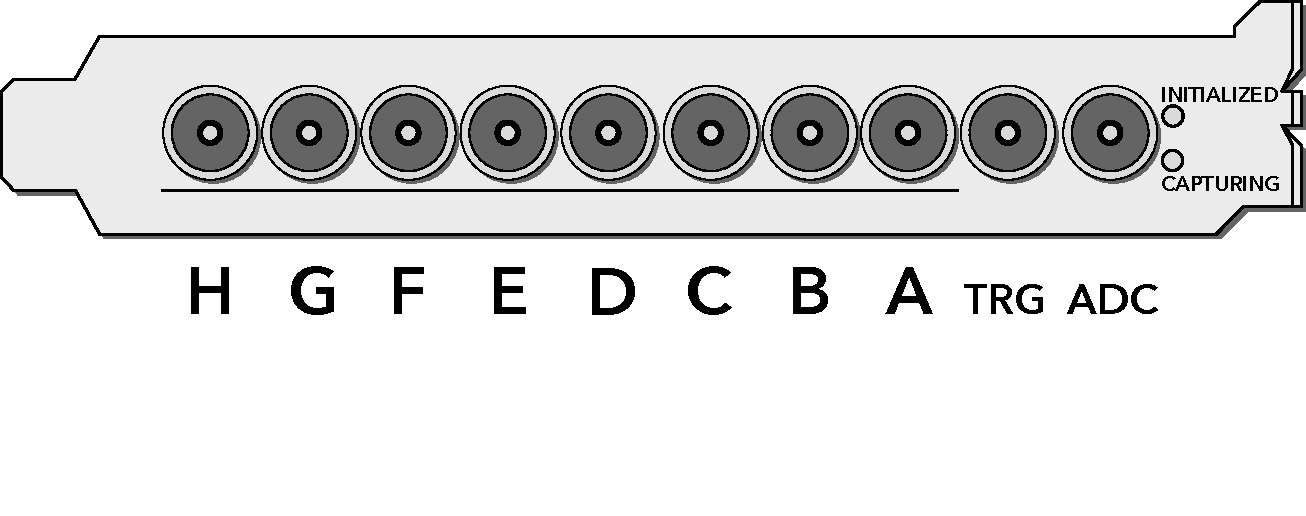
\includegraphics[width=0.6\textwidth]{figures/xHPTDC8_Slotblende.pdf}
			}{
				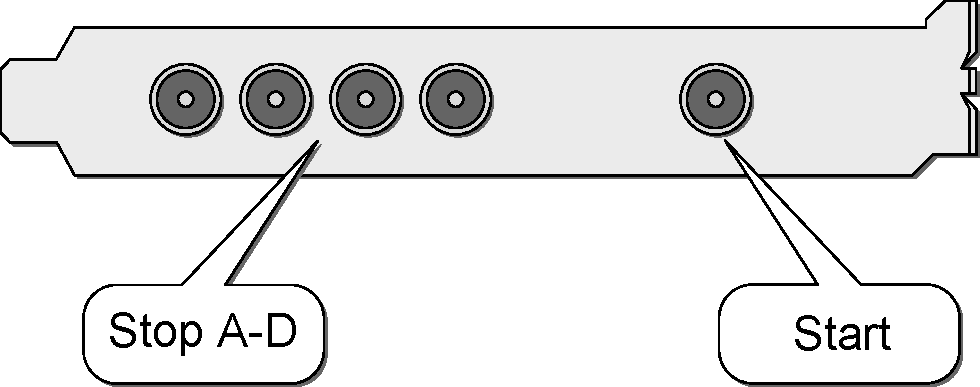
\includegraphics[width=0.6\textwidth]{figures/xTDC4_Slotblende.pdf}
			}
			\caption{Input connectors of the \deviceName\ on the PCIe bracket.\label{fig:bracket}}
		\end{center}
	\end{figure*}
	%
	\begin{figure*}[hb]
		\begin{center}
			\ifxHPTDC{
				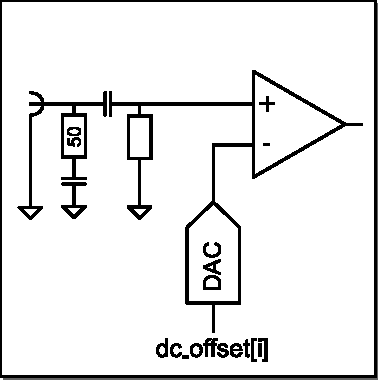
\includegraphics[width=0.3\textwidth]{xhptdc/figures/InputCircuit.pdf}
			}{
				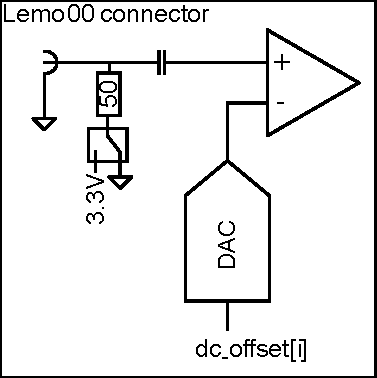
\includegraphics[width=0.3\textwidth]{figures/InputCircuit.pdf}
			}
			\caption{Input circuit for each of the input channels.\label{fig:inputcirc}}
		\end{center}
	\end{figure*}
	%

	Lemo-00 connectors are used for input connection. The inputs are AC-coupled and have an impedance of 50$\Omega$. 
	A schematic of the input circuit is shown in Figure \ref{fig:inputcirc}. 
	The digital threshold for any input can be adjusted to comply with a multitude of single ended signaling standards.
	The threshold can also be used to configure the input for either positive or negative pulses.
	
	
	The connectors can also be used as outputs. 
	\ifxHPTDC{AC-coupled}{DC-coupled} output pulses for automatic internal triggering and control of external devices 
	can be generated using the TiGer timing pattern generator. See section \ref{cp:tiger} for details on TiGer. 
	%
		\begin{figure*}[ht]
			\begin{center}
				\ifxHPTDC{
					\includegraphics[width=0.7\textwidth]{xhptdc/figures/xHPTDC8_schematic.pdf}
				}{
					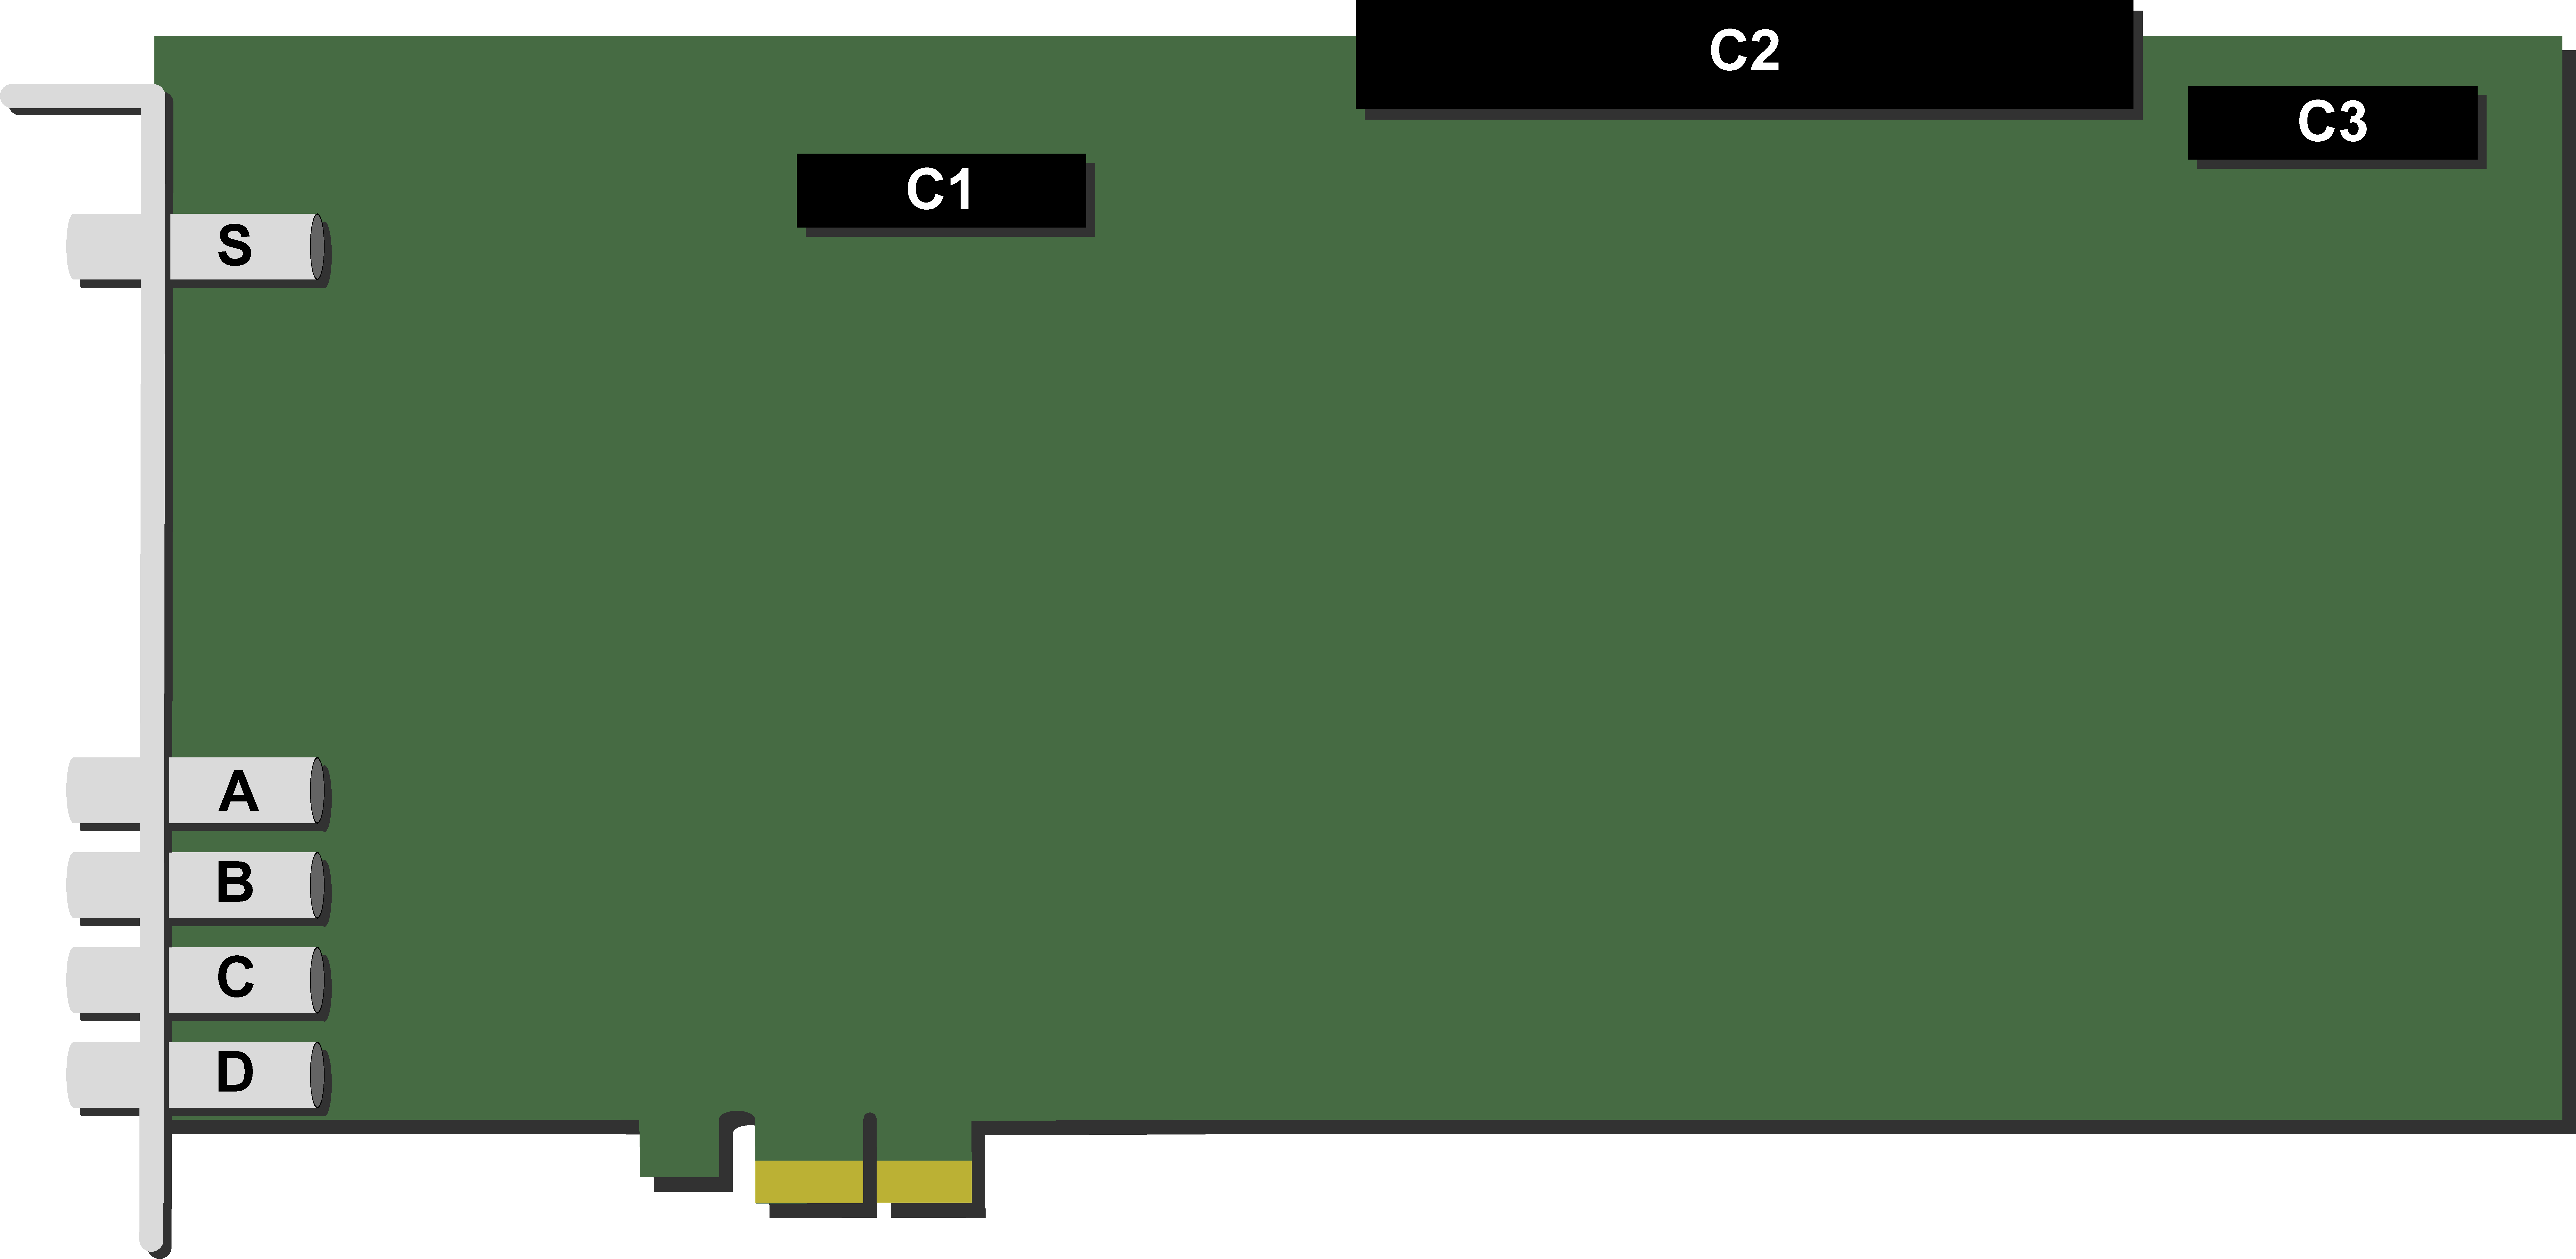
\includegraphics[width=0.7\textwidth]{figures/xTDC4_schematic.pdf}
				}
				
				\caption{Schematic view of a \deviceName\ board showing the inter-board connectors.\label{fig:schematics}}
			\end{center} 
		\end{figure*}
	%

	Furthermore, three inter-board connectors can be found at the top edge of the \deviceName\ board, 
	as displayed in Figure \ref{fig:schematics}. 
	Connector J25 is reserved for future use. The pinout of connector J12 is shown in Table \ref{J12} and the pinout of connector J6 is depicted in Table \ref{J6}.
	\ifxHPTDC{Connector J2 is a coax clock input that must receive a 10 MHz clock if multiple boards are used in together as described in section \ref{multiboard}.}{}

	\begin{table}
	\begin{small}
		\begin{center}
			\begin{tabular}{|c|c|}
				\hline
				Pin & Name\\
				\hline\hline
				1, 2 & GND\\
				\hline
				3, 4 & external CLK in N, external CLK in P\\
				\hline
				5, 6 & GND\\
				\hline
				7, 8 & reserved/NC\\
				\hline
				9, 10 & GND\\
				\hline
				11, 12 & reserved/NC\\
				\hline
				13, 14 & GND\\
				\hline
				15, 16 & reserved/NC\\
				\hline
				17, 18 & GND\\
				\hline
				19, 20 & reserved/NC\\
				\hline
				21, 22 & GND\\
				\hline
				23, 24 & reserved/NC\\
				\hline
				25, 26 & GND\\
				\hline
				27, 28 & reserved/NC\\
				\hline
				29, 30 & GND\\
				\hline
				31, 32 & reserved/NC\\
				\hline
				33, 34 & GND\\
				\hline
			\end{tabular}
			\caption{Pinout of connector J12.}
			\label{J12}
		\end{center}
	\end{small}
	\end{table}

	\begin{table}
	\begin{small}
		\begin{center}
			\begin{tabular}{|c|c|}
				\hline
				Pin & Name\\
				\hline\hline
				1 & +3.3 V\\
				\hline
				2 - 9 & reserved/NC\\
				\hline
				10 & GND\\
				\hline
			\end{tabular}
			\caption{Pinout of connector J6.}
			\label{J6}
		\end{center}
	\end{small}
	\end{table}

%%%%%%%%%%%%%%% multiboard
\ifxHPTDC{
	\section{Synchronizing multiple boards}
		\label{multiboard}
		If more than eight TDC inputs are required, up to eight boards can be synchronises within a system. 
		
		The \deviceName\ API described in chapter \ref{cp:api} manages up to eight boards automatically
		and provides a single data stream that contains sorted hit data from all boards in chronological order. 
		Channel A of each board is assigned channel number \textsf{board\tu index} $\cdot 10$. 
		The \textsf{board\tu index} is assigned to the boards in the order of the serial numbers starting at 0.

		\subsection{Connecting multiple boards}
			The boards must each receive a common 10~MHz clock on connector J2. The connector is inside the PC enclosure. 
			Connectors J12 of all boards must be connected with a flat band cable with a terminator at each end. 
			Cable and Terminator are available from cronologic. See figure \ref{fig:multiboard} for a wiring example.
			%
			\begin{figure*}[ht]
				\begin{center}
					\includegraphics[width=1\textwidth]{xhptdc/figures/multiboard.pdf}				
					\caption{Synchronising multiple boards with a ClockBox.\label{fig:multiboard}}
				\end{center} 
			\end{figure*}
			%
		\subsection{ClockBox}
			For systems of up to four boards cronologic offers the ClockBox product that conveniently makes four clock signals evailable 
			inside the PC enclosure. For use with the \deviceName, jumper JP3 of the CLockBox must be set as shown in Figure \ref{fig:clockbox} to set the clock frequency to 10~MHz. 
			%
			\begin{figure*}[ht]
				\begin{center}
					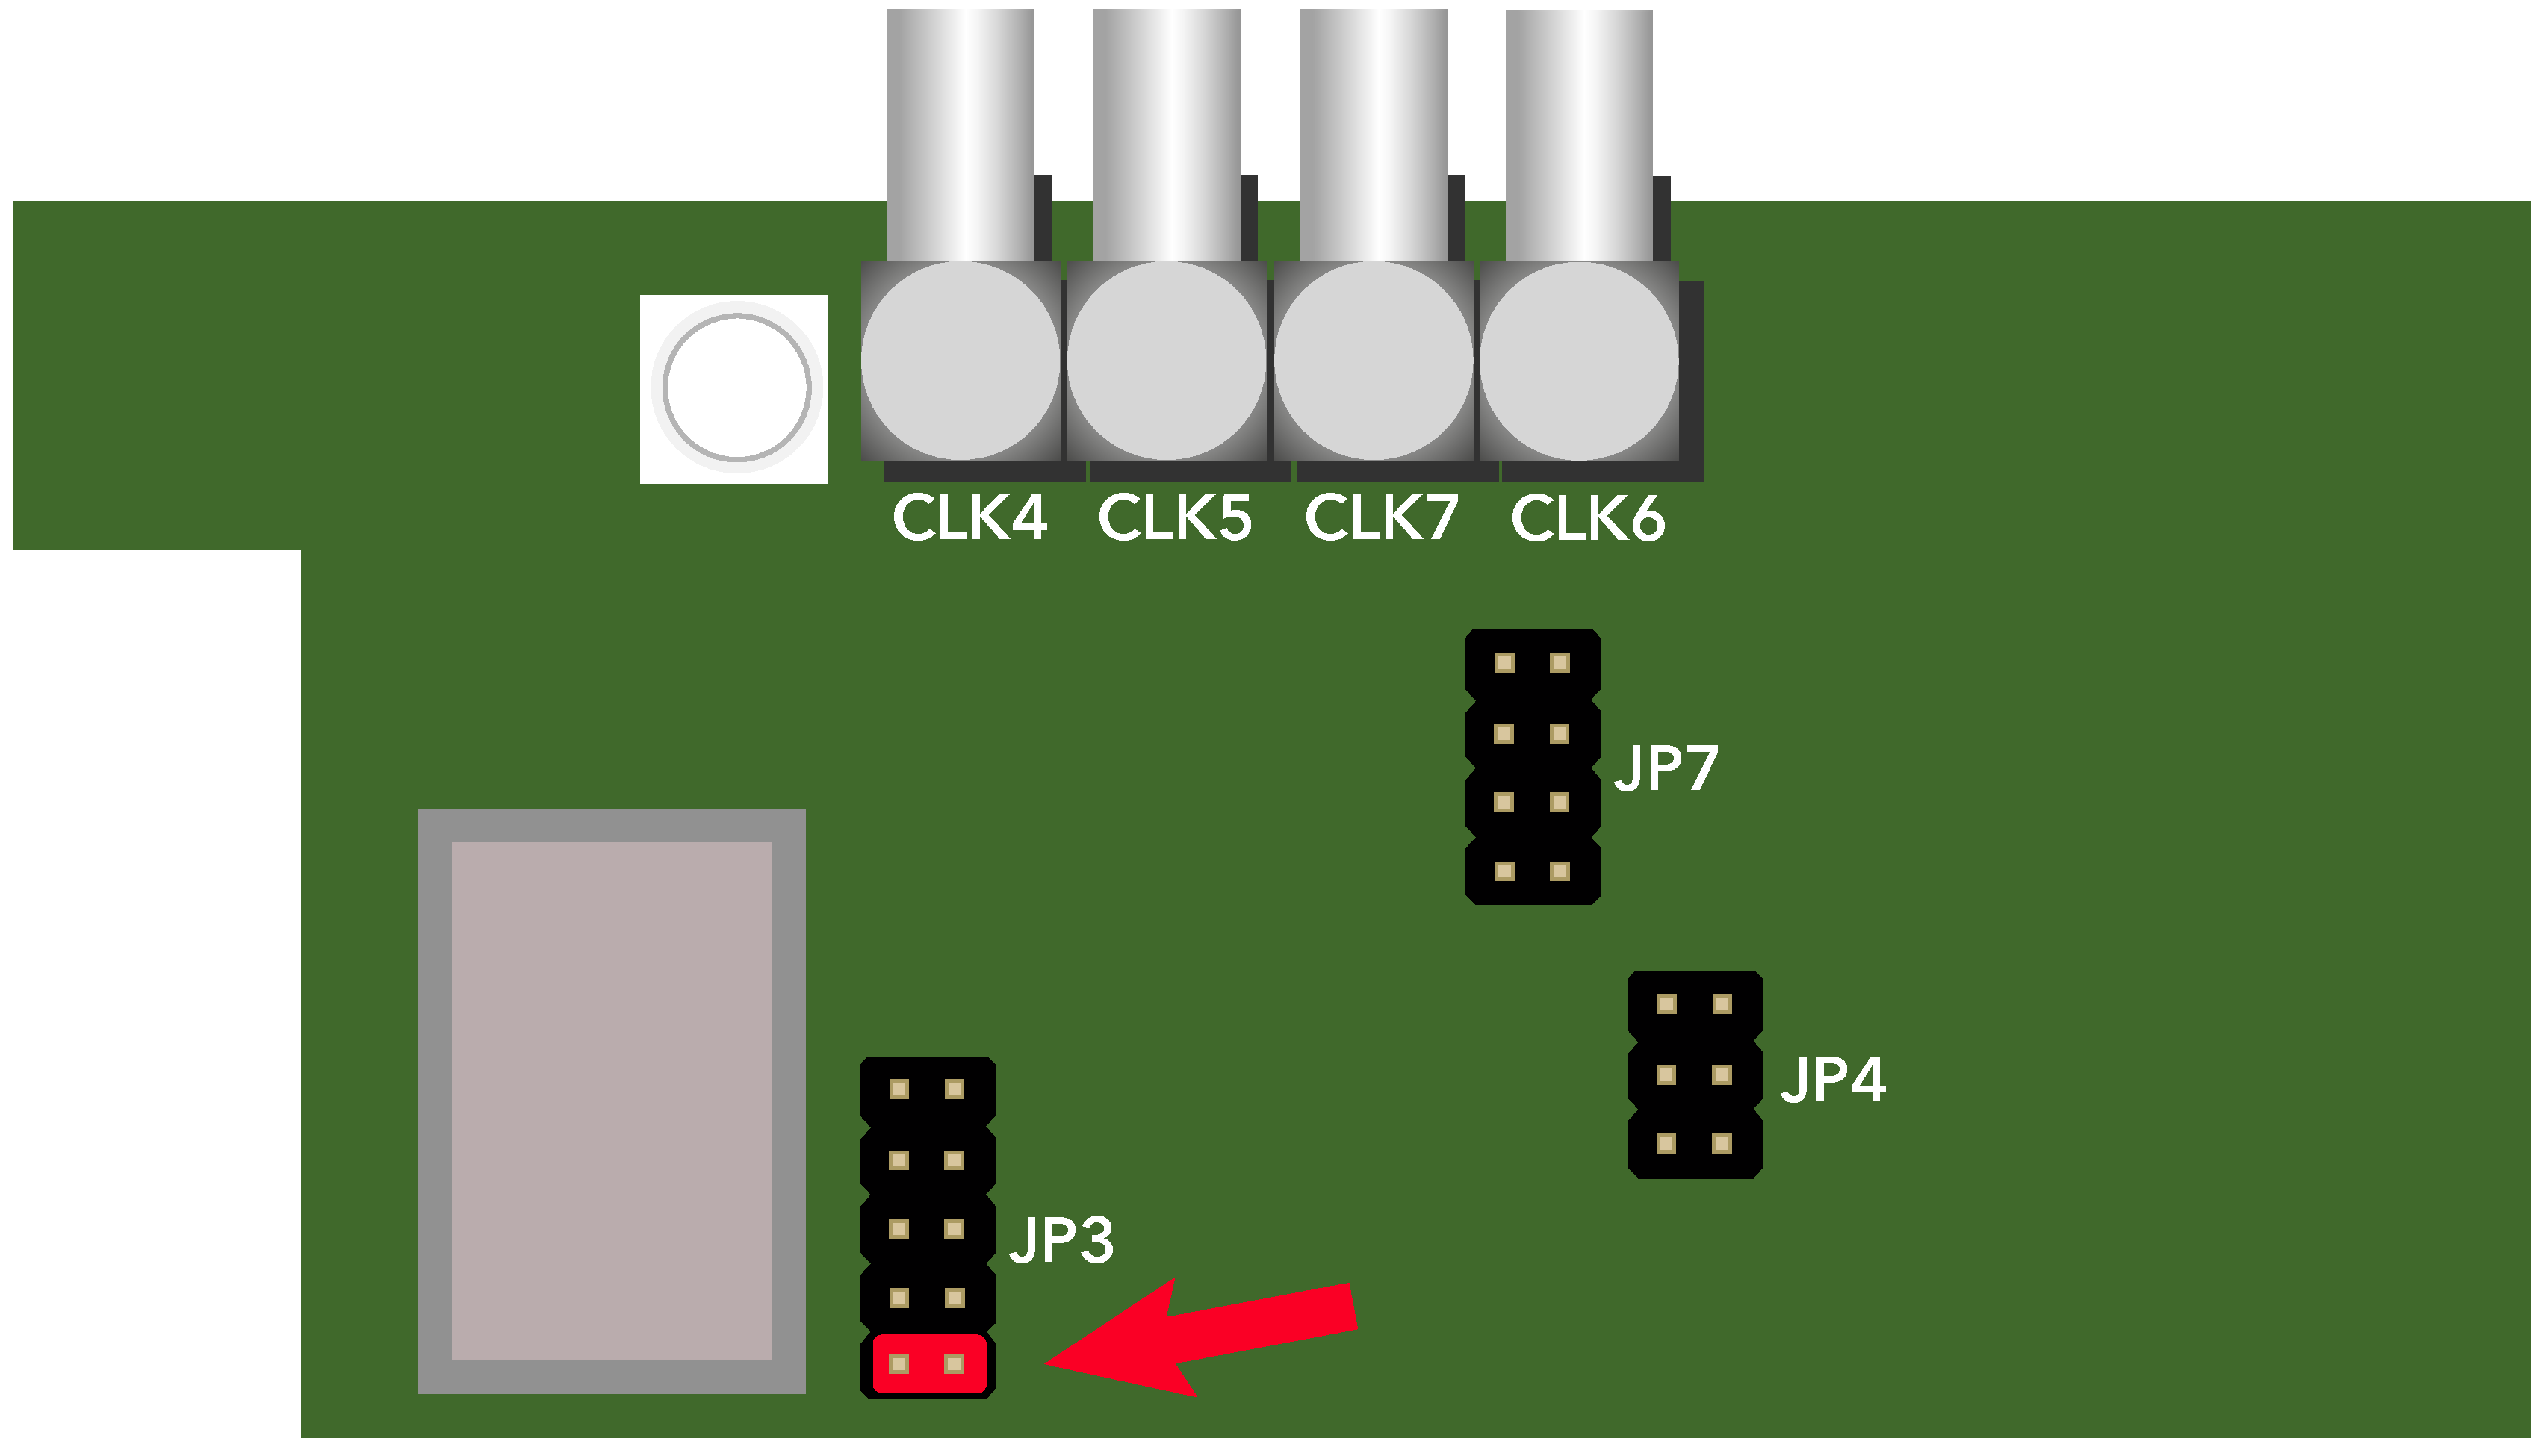
\includegraphics[width=0.5\textwidth]{xhptdc/figures/clockbox.pdf}				
					\caption{ClockBox jumper setting for 10~MHz.\label{fig:clockbox}}
				\end{center} 
			\end{figure*}
			%
		
		\subsection{Crates for multiple boards}
			Most PC mainboards don't have enough PCIe slots to support eight \deviceName s. 
			We offer external enclosure called "Ndigo Crate" that PCIe-over-cable technology to extend the number of available slots in a system.
			The extension is fully transparent to the host system. There are no additional drivers require. 
			Please see the \href{https://www.cronologic.de/products/pcie/pcie-crates}{product page} at our website \url{www.cronologic.de}.  
		

	

}{}




	




	\chapter{\deviceName\ Functionality}
		\txh{ %TimeTagger Version
The \deviceName\ is a ``classic'' common start time-to-digital converter. 

It records the time difference between a leading or trailing edge on the start input to the leading and trailing edges of the stop inputs. 
Rising and falling edges of the stop channel A-D can be enabled individually. 
The measurements are quantized to $500$~ps for -2G devices and tp $1000$~ps for -1G devices. 
The timestamps are recorded in integer multiples of a bin size of $500$~ps for both board types to simplifiy setups where data from differnt board types is combined.
Transitions of the input signals are called hits. To reliably detect hits the signal has to be stable for more than one quantisation interval before and after the edge.  
Triggers on the start channel must not occur less than 5ns apart. The \deviceName\ records events without dead time at a readout rate of about 48MHits/s.
} { %xTDC4 Version
The \deviceName\ is a ``classic'' common start time-to-digital converter. 

It records the time difference between leading or trailing edges on the start input and the stop inputs. 
Each stop channel A-D can be enabled individually. 
The standard deviation of the timestamps is approx. $8$~ps. 
The timestamps are recorded in integer multiples of a bin size of $5/(3\cdot 128) = 13.0208\overline{3}$~ps. 
The data acquisition can be limited to rising or falling signal transitions. 

The maximum trigger rate on the start channel is 4~MHz.

\subsection{Handling of Difficult Hits}
    \label{difficulthits}
    Transitions of the input signals are called hits. To measure all hits with the maximum resolution the hits must fulfill all criteria set forth in this document.
    However, the \deviceName does include mechanisms to provide as much information as possible for hits that fall out of these specs.

    To reliably detect hits the signal has to be stable for at least $900$~ps before and after the edge that is to be measured. 
    Pulses as short as $250$~ps are usually detected at full resolution but have a significant chance to be assigned to the wrong group or appear out of order. 
    For these hits bit 7 in the data word is set. See section \ref{flags} for more information on the data format.

    Between multiple hits on a stop channel a deadtime of approximately $5$~ns is required for full resolution. 
    Hits that are closer together will only be reported with a resolution of $5/6~ns = 833,\overline{3}~ps$. For these hits both bits 6 and 7 are set.

    Data is copied from the 15-entry L0 FIFO to the larger downstream FIFOs at a reate of about $12$~MHz per channel. 
    If the L0 FIFO overflows the hig resolution measurement of some hits will be discarded. 
    In this case a measurement from an alternative TDC wil be used that has a resolution of about $150$~ps. 
    For these hits bit 6 in the data word will be set
} { %xHPTDC8 version
    The \deviceName\ is a streaming time-to-digital converter. It records the timestamps of changes at the inputs A-H in an infinite stream. 
    A flexible grouping mode is available that can emulate common-start or common-stop behaviour. See section \ref{grouping} for details.

    For each channel it can be selected individually whether rising or falling edges are recorded. It is not possible to record both edges of the same channel. 
    The timestamps are recorded in integer multiples of a bin size of $5/(3\cdot 128) = 13.0208\overline{3}$~ps. 
    There must be at least 5~ns between consecutive hits on the same input channel to be detected reliably. 
    The \deviceName\ records events without dead time at a readout rate of about 48MHits/s.
} 
		\section{Grouping and Events}
\label{grouping}
\ifxHPTDC{
    If \textsf{config.tdc\tu mode} is set to \textsf{\PREFIX TDC\tu MODE\tu GROUPING} the TDC will operate in grouping mode. 
    In grouping mode each call to \textsf{xhptdc8\tu read\tu hits()} will return a group of timestamps relative to some trigger event. 
    Otherwise the call returns all available timestamps as absolute timestamps counting upwards from \textsf{xhptdc8\tu start\tu capture()}
}{} 

In typical applications a start hit is followed by a multitude of hits on e.g. a detector. 
The hits recorded are managed in groups (which are called ``events'' in some applications). 
%
\begin{figure*}[ht]
    \begin{center}
        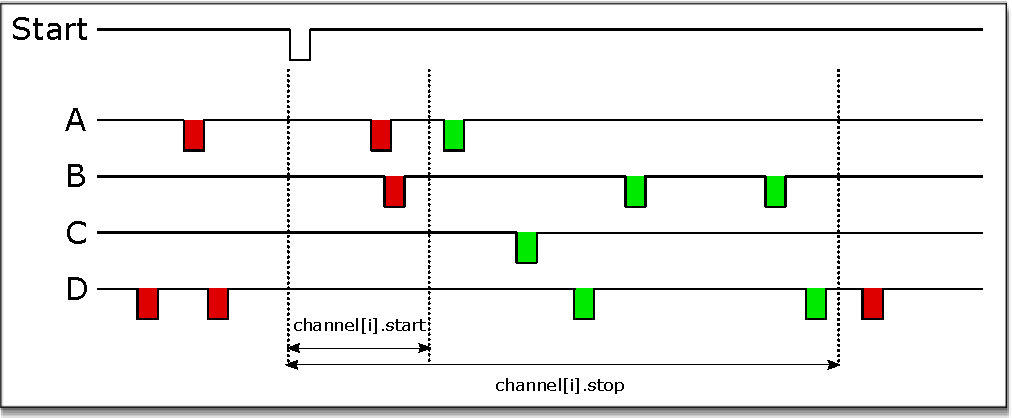
\includegraphics[width=0.7\textwidth]{figures/grouping.pdf}
        \caption{Acquired hits are merged to groups as explained in the text.\label{fig:grouping}}
    \end{center}
\end{figure*}
%

Figure \ref{fig:grouping} shows a corresponding timing diagram. The user can define the range of a group, i.e. the time window within which hits 
on the stop channels are recorded, in software. Hits occurring outside of that time window are discarded. 
 Different ranges can be set for each of the 4 stop channels by setting corresponding values for \textsf{config.grouping.start} and \textsf{.stop} values.

 \ifxHPTDC{
     The values are configured in picoseconds. Negative values can be used in common stop applications.
     \[ -2^{31} <= start <= stop <= 2^{31}-1 \]
 }{
    The values need to be set as multiples of the bin size and must not be negative.
    \[ 0 <= start <= stop <= 2^{16}-1 \]
 }

 In single board setups it is recommended to also configure the gating blocks accordingly. 
 This prevents data from beeing read out that is discarded by the grouping code anyway. 
 Plase note that the grouping parameters are given in picoseconds while the gating blocks are configured in cycles of the 150~MHz clock.


		\lstset{
	language=[Visual]C++,
	keywordstyle=\bfseries\sffamily\color[rgb]{0,0,1},
	identifierstyle=\sffamily,
	commentstyle=\color[rgb]{0.133,0.545,0.133},
	stringstyle=\sffamily\color[rgb]{0.627,0.126,0.941},
	showstringspaces=false,
	basicstyle=\small,
	numberstyle=\footnotesize,
	numbers=left,
	stepnumber=1,
	numbersep=10pt,
	tabsize=2,
	breaklines=true,
	prebreak = \raisebox{0ex}[0ex][0ex]{\ensuremath{\hookleftarrow}},
	breakatwhitespace=false,
	aboveskip={1.5\baselineskip},
	columns=fixed,
	upquote=true,
	extendedchars=true,
}

\section{Auto Triggering Function Generator\label{cp:AutoTriggeringFunctionGenerator}}
Some applications require internal periodic or random triggering. The \deviceName\ function generator provides this functionality.\par

The delay between two trigger pulses of this trigger generator is the sum of two components: A fixed value M and a pseudo random value given by the exponent N. \par

The period is

\begin{align}
    T = 1 + M + [1...2^N]
\end{align}

clock cycles \ifxHPTDC{of the 150~MHz clock}{with a duration of $4~ns$ per cycle}.\par

The trigger can be used as a source for the TiGer unit (see Section \ref{cp:tiger}).


\section{Timing Generator (TiGer)\label{cp:tiger}}
Each digital LEMO-00 input can be used as a \ifxHPTDC{AC coupled}{LVCMOS} trigger output. 
The TiGer function can be configured independently for each connector. 
See Section \ref{cp:tigerblock} for a full description of the configuration options.
% 
\begin{figure*}[ht]
    \begin{center}
        \ifxHPTDC { 
            % this is an XCIrcuit drawing  convertex from postscript with 
            %ps2pdf.exe -dEPSCrop xhptdc8_trigger_matrix.ps
            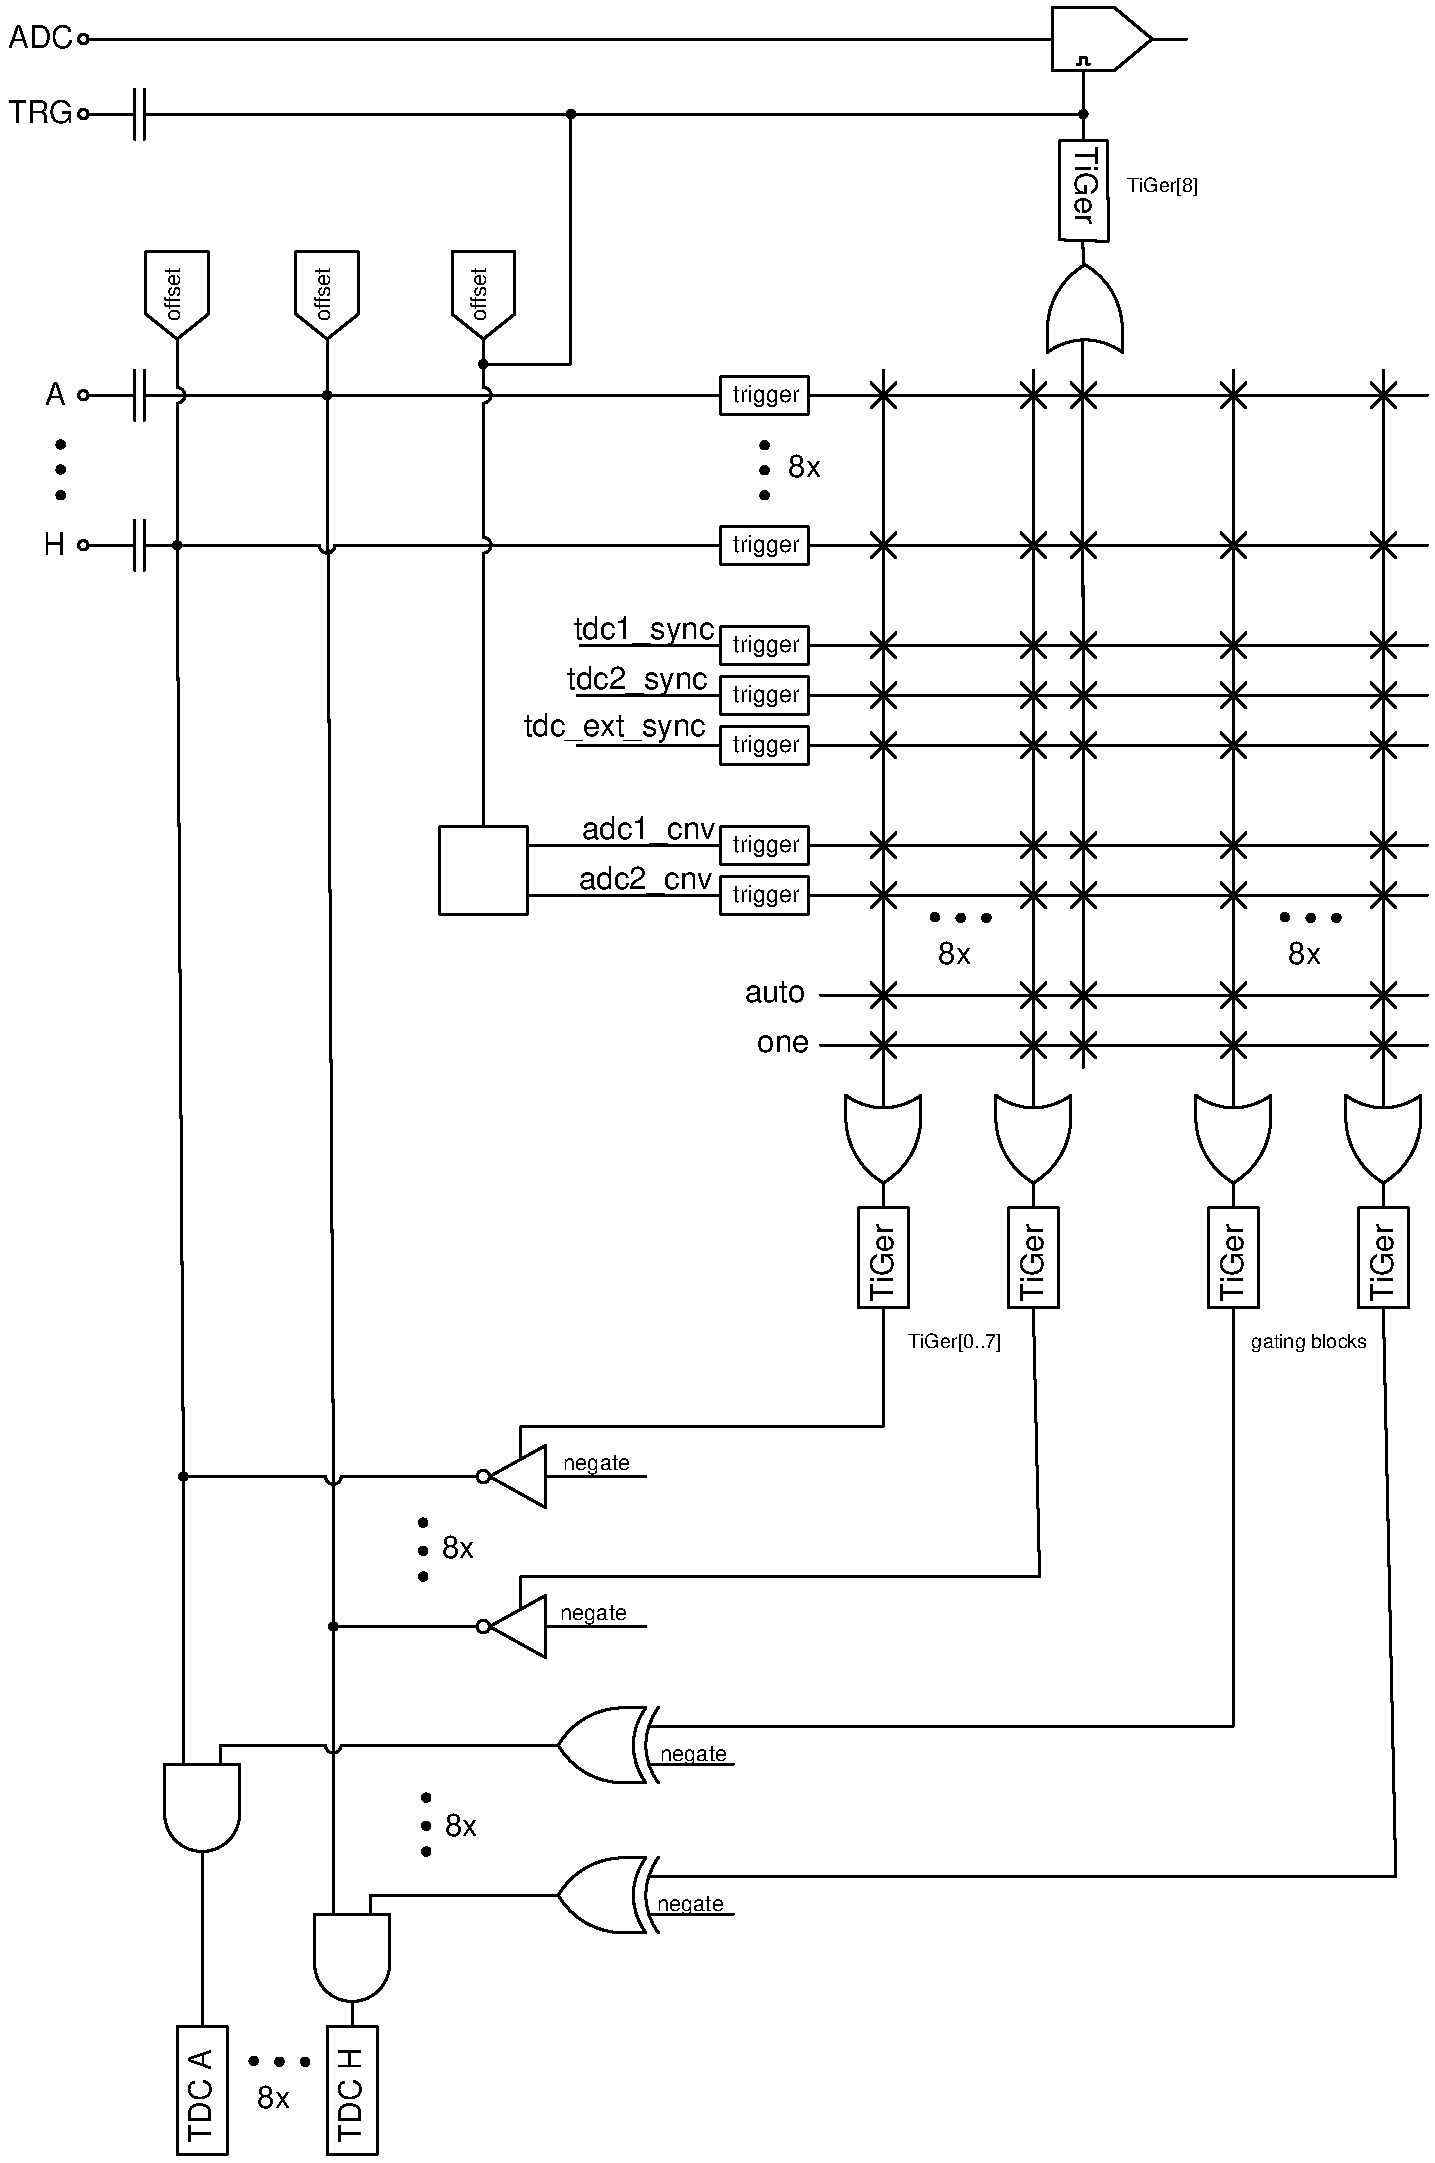
\includegraphics[width=0.6\textwidth]{xhptdc/figures/xhptdc8_trigger_matrix.pdf}
        }{
            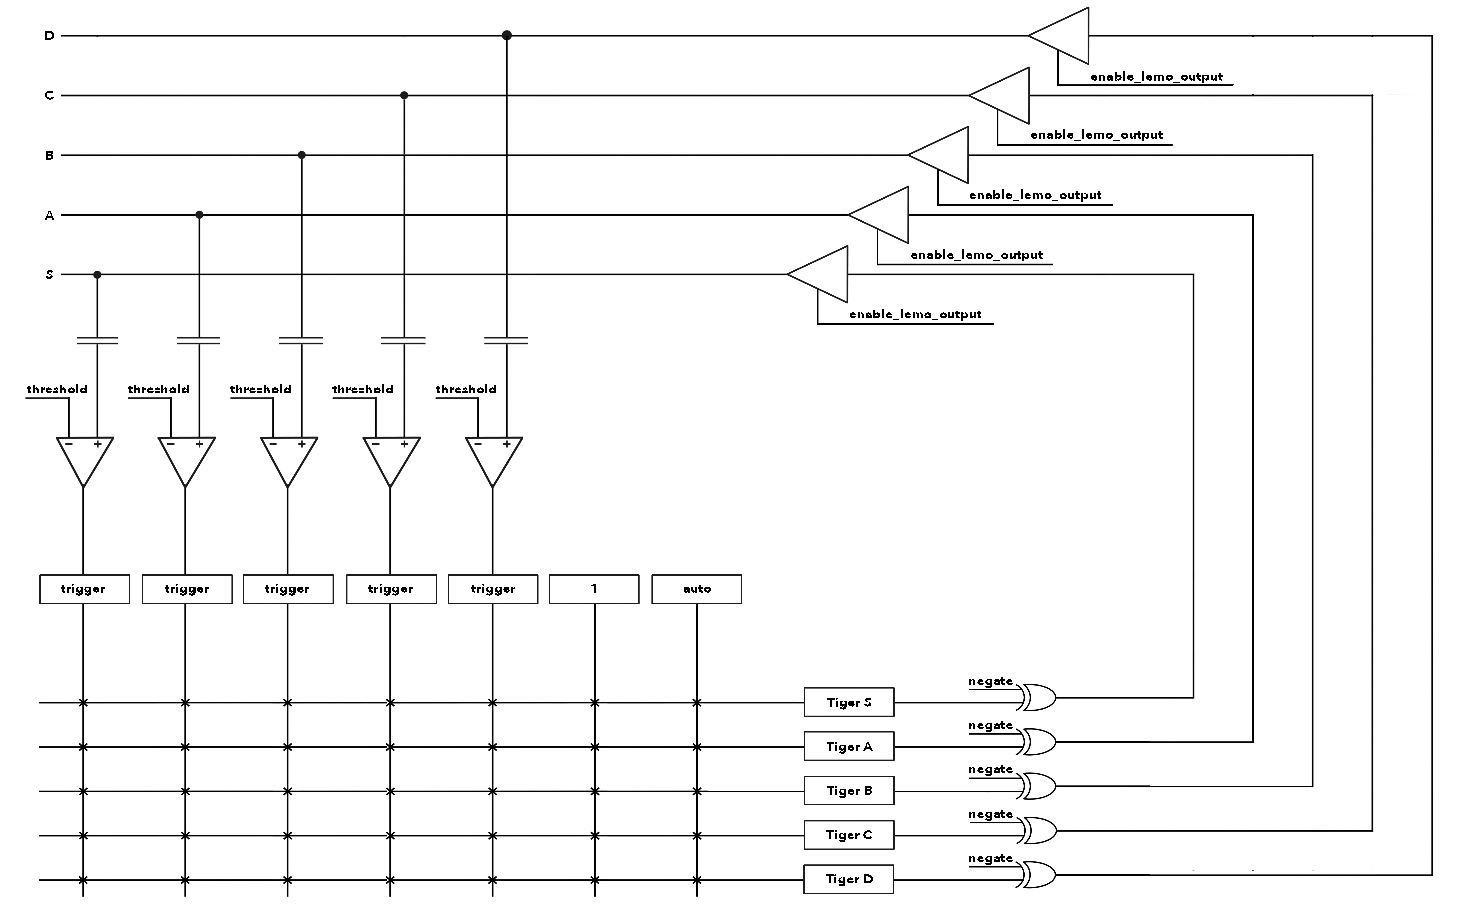
\includegraphics[width=0.7\textwidth]{figures/xTDC4_tiger_matrix.pdf}
        }
        \caption{TiGer blocks can generate outputs that are also available on inputs.\label{fig:matrix}} 
    \end{center}
\end{figure*}
%

Figure \ref{fig:matrix} shows how the TiGer blocks are connected. They can be triggered by an OR of an arbitrary combination of inputs, 
including the auto trigger. Each TiGer can drive its output to its corresponding LEMO connector. This turns the connector into an output. 

When there is an ADC trigger pulse on the TRG connector, either of the two on board ADCs is triggered in an unpredictable pattern. 
If the TRG input shall be used as a trigger the trigger sources must be contain both \textsf{ADC1\tu CNV} and \textsf{ADC21\tu CNV}.

The trigger sources with names ending in \textsf{\tu sync} are managed by the driver for multi board setups and must be left unchanged by the user.

\ifxHPTDC{
	The TiGer outputs are AC coupled to the connector. They can be operated in one of the following modes:
	\paragraph*{\textsf{\PREFIX TIGER\tu OFF}} 
		No signal is output to the connetor. 
	\paragraph*{\textsf{\PREFIX TIGER\tu OUTPUT}} 
		In this mode the connector is input only. Pulses are unipolar with 2V amplitude. 
		Connected hardware must not drive any signals to connectors used as outputs, as doing so could damage both the \deviceName and the external hardware. 
		We recommend to only use short pulses to avoid undesirable baseline shift due to the AC coupling, but the device does not pose any restrictions on the duty cycle. 
		This mode can be used as a clock output with a frequency of $75/N$~MHz for integer $N$.
	\paragraph*{\textsf{\PREFIX TIGER\tu BIDI}} 
		In this mode the TiGer creates unipolar pulses with 1~V amplitude. The connector can still be used as an input. 
		Use short pulses to keep the propability of collision and the effect on the baseline low.	
	\paragraph*{\textsf{\PREFIX TIGER\tu BIPOLAR}} 
		In this mode the connector creates bipolar pulses with 1~V amplitude. The connector can still be used as an input. 
		The pulses have no effect on the baseline offset. 
		TiGer should be configured with $stop = start$ for minimum width bipolar pulses of $2 \times 6.\overline{6}~ns$. 
		The maximum bipolar pulse width is \textsf{XHPTDC8\tu TIGER\tu MAX\tu BIPOLAR\tu PULSE\tu LENGTH = 15}.    
}{
	The TiGer is DC coupled to the connector. Connected hardware must not drive any signals to connectors used as outputs, 
	as doing so could damage both the \deviceName\  and the external hardware.
	Pulses that are short enough for the input AC coupling are available as input signals to the \deviceName. 
	This can be used to measure exact time differences between the generated output signals and input signals on other channels.
}
\ttinput{Tiger_Example.tex}	

\ifxHPTDC{
	\subsection{Triggering the ADC with the TiGer}
		\label{adctiger}
		There is a ninth TiGer that is connected to the trigger input of the ADC. See section \ref{adc} for additional information on the ADC. 

		The ADC TiGer can be used with retrigger enabled to periodically sample ADC data. 
		The period should be no shorter than 300~ns or 45 TiGer clocks.

		The ADC TiGer can also be used to sample voltages at a time relative to one of the TDC inputs. In this case 
		stop should be set to at least 45 to ensure that the sample period criterion is met even when pulses
		arrive in quick succession. A typical application would be to sample some slow control voltage once per start signal.

	\section{Gating}
		Each TDC channel has a second TiGer block that functions as a gate as shown in figure \ref{fig:matrix}. 
		While that output of that gating block is active no hits are recorded in that channel.
		If the block is negated hits are only recorded while the gating block is active.
		
		This is a useful feature in setups where the trigger creates a lot of noise.
		A suitable configuration of the gating block can reduce the bandwidth and buffer usage significantly.
		Gating is performed before the L0 buffer. Grouping is performed in software after readout. 
		
	\section{Triggerable ADC}
		\label{adc}
		The \deviceName\ is equipped with a triggerable ADC. 
		Whenever there is a rising edge on the ADC trigger connector, 
		the voltage on the ADC input connector is sampled. 
		The result is inserted as a packet with timestamp and ADC value into the readout data stream.

		The ADC trigger also is connected to the output of a TiGer block. 
		This can be used to to trigger the ADC periodical or relative to one of the TDC input as described in section \ref{adctiger}

		The ADC triggers should not be closer than 300ns apart.

		There are two interleaved ADCs  to ensure that there is always an ADC available even during readout. 
		This is exposed to the user both in the output data format and in the TiGer and Gating trigger sources.
		When using the ADC trigger as a trigger for Gating or TiGer both trigger sources shall be set to the same value.
		During readout the user shall not distinguish between data from the two ADCs unless advanced calibration is 
		desired for the ADC data. In that case the two ADCs should be treated separately.   

}{} 

	\chapter{Driver Programming API\label{cp:api}} 
		% also includes common/StructConfig.tex and common/InfoStructs.tex
		\ifxHPTDC{
	\newcommand{\device}{\cronvar{\prefix manager}{*xhptdc8\tu mgr}}
	\newcommand{\deviceindex}{\device, \cronvar{int}{index}}
	\newcommand{\deviceconfig}{\device}
	\newcommand{\initparameters}{xhptdc8manager\tu init\tu parameters}
}{
	\newcommand{\device}{\cronvar{\prefix device}{*device}}
	\newcommand{\deviceindex}{\device}
	\newcommand{\deviceconfig}{\deviceindex}
	\newcommand{\initparameters}{\prefix init\tu parameters}
}

The API is a DLL with C linkage.\par

The functions provided by the DLL are declared in \textsf{\txh{TimeTagger4}{xTDC4}{xHPTDC8}\tu interface.h}.

\section{Constants}
\ifxHPTDC{
	\crondef{XHPTDC8MANAGER\tu DEVICES\tu MAX 8}\\
	The maximum number of boards supported by the device manager.

	\ttdef{TDC\tu CHANNEL\tu COUNT 8}\\
	The number of TDC input channels.\par

	\ttdef{GATE\tu COUNT 8}\\
	The number of gating blocks. One for each TDC input.\par

	 \ttdef{TIGER\tu COUNT 9}\\
	The number of timing generators. One for each TDC input and one for the adc trigger.\par

	 \ttdef{TRIGGER\tu COUNT 16}\\
	The number of potential trigger sources for the timing generators. One for each TDC input 
	\ifxHPTDC{}{, one for the Start input} plus some specials. 
	 See Section~\ref{cp:tigerblock} for details.\par

}{ 
	\ttdef{CHANNEL\tu COUNT 4}\\
	The number of TDC input channels.\par

	 \ttdef{TIGER\tu COUNT 5}\\
	The number of timing generators. One for each TDC input and one for the start input.\par

	 \ttdef{TRIGGER\tu COUNT 16}\\
	The number of potential trigger sources for the timing generators. One for each TDC input, one for the Start input plus some specials. 
	 See Section~\ref{cp:tigerblock} for details.\par
}


\section{Driver Information}

	Even if there is no board present the driver revision can be queried using these functions.

	\ttvar{int}{get\tu driver\tu revision()}\\
	Returns the driver version, same format as \textsf{\prefix static\tu info.driver\tu revision}. 
	This function does not require a \deviceName\ board to be present.

	\ttvar{const char*}{get\tu driver\tu revision\tu str()}\\
	Returns the driver version including SVN build revision as a string. 

	\ttvar{int}{count\tu devices(}\cronvar{int}{*error\tu code}, \cronvar{char}{**error\tu message)}\\
	\label{countdevices}
	Returns the number of boards present in the system that are supported by this driver.\par


\section {Initialization}

		\ttvar{int}{close(}\device )\\
		Finalizes the driver for this device.

		\ttvar{int}{get\tu default\tu init\tu parameters(}\cronvar{\initparameters}{ *init)}\\
		Sets up the standard parameters. Gets a set of default parameters for \textsf{\prefix init()}. This must always be used to initialize the \textsf{\prefix init\tu parameter()} structure.\par

		\cronvar{\prefix \ifxHPTDC{manager}{device} *}{\prefix init(}\cronvar{\initparameters}{*params}, \\ 
		\cronvar{int}{*error\tu code}, \cronvar{char}{**error\tu message)}\\
		Opens and initializes the \deviceName\ board with the given index. 
		The user must provide pointers to memory locations where the driver can store return values.\\
		\textsf{error\tu code} shall point to an integer for the error code. \\
		\textsf{error\tu message} must point to a pointer to char. The driver will allocate a buffer for zero terminated error messages and store the address of the buffer in the location provided by the user.\par

		The paramter \textsf{params} is a structure of type \textsf{\prefix init\tu parameters} that must be completely initialized.\par

%%%%%%%%%%%%%%%%% struct init_parameters

		\subsection{Structure \initparameters}
			\cronvar{int}{version}\\
			The version number. Must be set to \textsf{\PREFIX API\tu VERSION}.\par

			\ifxHPTDC{}{
				\cronvar{int}{card\tu index}\\
				The index in the list of \deviceName\ boards that should be initialized.\\
				There might be multiple boards in the system that are handled by this driver as reported by \textsf{\prefix count\tu devices}. This index selects one of them. Boards are enumerated depending on the PCIe slot. 
				The lower the bus number and the lower the slot number the lower the card index.\par

				\cronvar{int}{board\tu id}\\
				the global index in all cronologic devices.\\
				This 8 bit number is filled into each packet created by the board and is useful if data streams of multiple boards will be merged. If only \deviceName\ cards are used this number can be set to the \textsf{card\tu index}. 
				If boards of different types that use a compatible data format are used in a system each board should get a unique id.
				Can be changed with \textsf{int \prefix set\tu board\tu id\allowbreak(\prefix device *device, int board\tu id)}.\par
			}

			\cronvar{\tu \tu int64}{buffer\tu size\ifxHPTDC{}{[8]}}\\
			The minimum size of the DMA buffer.\\
			If set to 0 the default size of 16~MByte is used. 
			\ifxHPTDC{}{For the \deviceName\ only the first entry is used.}\par

			\ifxHPTDC{}{
				\cronvar{int}{buffer\tu type}\\
				The type of buffer. Must be set to 0.
				\begin{description}
					\item[]  \ttdef{BUFFER\tu ALLOCATE   0}
					\item[]  \ttdef{BUFFER\tu USE\tu PHYSICAL   1}  // unsupported
				\end{description}
			

				\cronvar{\tu \tu int64}{buffer\tu address}\\
				This is set by \prefix init() to the start address of the reserved memory.\\ 
				The buffers will be allocated with the sizes given above. Make sure that the memory is large enough.\par
			}

			\cronvar{int}{variant}\\
			Set to 0. Can be used to activate future device variants such as different base frequencies.\par

			\cronvar{int}{device\tu type}\\
			A constant for the different devices of cronologic \textsf{CRONO\tu DEVICE\tu *}.\\
			Initialized by \textsf{\prefix get\tu default\tu init\tu parameters()}. This value is identical to the PCI Device ID. Must be left unchanged.

			\begin{tabular}{ll}
				\crondef{CRONO\tu DEVICE\tu HPTDC}       & 0x1 \\
				\crondef{CRONO\tu DEVICE\tu NDIGO5G}     & 0x2 \\
				\crondef{CRONO\tu DEVICE\tu NDIGO250M}   & 0x4 \\
				\crondef{CRONO\tu DEVICE\tu xTDC4}       & 0x6 \\
				\crondef{CRONO\tu DEVICE\tu TIMETAGGER4} & 0x8 \\
				\crondef{CRONO\tu DEVICE\tu XHPTDC8}     & 0xC \\
				\crondef{CRONO\tu DEVICE\tu NDIGO6}      & 0xD \\
			\end{tabular}

			\cronvar{int}{dma\tu read\tu delay}\\
			The update delay of the write pointer after a packet has been sent over PCIe. Specified in multiples of 16~ns.
			Should not be changed by the user.\par

			\ifxHPTDC{
				\cronvar{int}{multiboard}\\
				Set if multiple devices shall be synchronized.\par
	
				\cronvar{int}{use\tu ext\tu clock}\\
				If set to 1 use external 10 MHz reference. If set to 0 use internal reference.\par

				\cronvar{int}{ignore\tu calibration}\\
				Leave at 0 to use device calibration data.\par
		
			}{
				\cronvar{int}{use\tu ext\tu clock}\\
				If set to 1 use external 10 MHz reference. If set to 0 use internal reference.\par	
			}
	

	
	% info structures
	\section{Status Information}
	

\subsection{Functions for Information Retrieval}
    The driver provides functions to retrieve detailed information on the board type, its configuration, settings and state. 
    The information is split according to its scope and the computational requirements to query the information from the board.
    
    \ifxHPTDC{
        The information is provided on a per board basis. The parameter \textsf{index} selects which board is queried.
    }{}

    \ttvar{int}{get\tu device\tu type}(\device)\\
    Returns the type of the device as \textsf{CRONO\tu DEVICE\tu \txh{TIMETAGGER4}{XTDC4}{XHPTDC8}}.\par

    \ttvar{const char*}{get\tu last\tu error\tu message(\device)}\\
    Returns most recent error message.\par

    \ttvar{int}{get\tu fast\tu info(}\deviceindex, \lb\cronvar{\prefix fast\tu info}{*info)}\\
    Returns fast dynamic information.\\
    This call gets a structure that contains dynamic information that can be obtained within a few microseconds.\par

    \ttvar{int}{get\tu param\tu info(}\deviceindex, \lb\cronvar{\prefix param\tu info}{*info)}\\
    Returns configuration changes.\\
    Gets a structure that contains information that changes indirectly due to configuration changes.\par


    \ttvar{int}{get\tu static\tu info(}\deviceindex, \lb\cronvar{\prefix static\tu info}{*info)}\\
    Contains static information.\\
    Gets a structure that contains information about the board that does not change during run time.\par 

   \ifxHPTDC{
        \ttvar{int}{get\tu temperature\tu info(}\deviceindex, \lb\cronvar{\prefix temperature\tu info}{*info)}\\
        Get temperature measurements from multiple sources on the board.

        \ttvar{int}{get\tu clock\tu info(}\deviceindex, \lb\cronvar{\prefix clock\tu info}{*info)}\\
        Get information on clocking configuration an status.

        \ttvar{const char *}{device\tu state\tu to \tu str(}\cronvar{int state)}\\
        Convert the state value from \textsf{\prefix fast\tu info.state} into a human readable string. 
   }{   
        \ttvar{int}{get\tu slow\tu info(}\deviceindex, \lb\cronvar{\prefix slow\tu info}{*info)}\\
        Returns slow dynamic information.\\
        The data reported in this structure requires milliseconds to be obtained. 
        The application should only call it in situations where the program flow can be blocked as long.\par
   } 

%%%%%%%%%%%%%%%%% static info

\subsection{Structure \prefix static\tu info}

This structure contains information about the board that does not change during run time. It is provided by the function \textsf{\prefix get\tu static\tu info}.\par

\cronvar{int}{size}\\
The number of bytes occupied by the structure.

\cronvar{int}{version}\\
A version number that is increased when the definition of the structure is changed. The increment can be larger than one to match driver version numbers or similar. Currently only version 0 is defined.\par

\cronvar{int}{board\tu id}\\
ID of the board.\\
\ifxHPTDC{
    All \deviceName\ boards in the system are numbered according in order of their serial numbers starting at zero.
    The channel A of a board has channel number $board\_id \cdot 10$. \par
}{}

\cronvar{int}{driver\tu revision}\\
Encoded version number for the driver.\\
The lower three bytes contain a triple level hierarchy of version numbers, e.g. 0x010103 encodes version 1.1.3.\\
The versionen adheres to the Semantic Versioning scheme as defined at \href{https://semver.org}{https://semver.org}. A change in the first digit generally requires a recompilation of user applications. 
Changes in the second digit denote significant improvements or changes that don't break compatibility 
and the third digit increments with minor bug fixes and similar updates that do not affect the API.\par

\cronvar{int}{driver\tu build\tu revision}\\
The build number of the driver according to cronologic's internal versioning system.

\cronvar{int}{firmware\tu revision}\\
Revision number of the FPGA configuration.

\cronvar{int}{board\tu revision}\\
Board revision number.\\
The board revision number can be read from a register. It is a four-bit number that changes when the schematic of the board is changed. This should match the revision number printed on the board.

\cronvar{int}{board\tu configuration}\\
Describes the schematic configuration of the board.\\
The same board schematic can be populated in multiple variants. This is a four bit-code that can be read from a register.

\cronvar{int}{subversion\tu revision}\\
Subversion revision id of the FPGA configuration source code.

\txh{
    \cronvar{int}{chip\tu id}\\
    Reserved.
}{
    \cronvar{int}{chip\tu id}\\
    16 bit factory ID of the TDC chip.
}{
    \cronvar{int}{chip\tu id[2]}\\
    16 bit factory ID for each of the TDC chips.
}\par

\cronvar{int}{board\tu serial}\\
Serial number.\\
With year and running number in 8.24 format. The number is identical to the one printed on the silvery sticker on the board.\par

\cronvar{unsigned int}{flash\tu serial\tu high}\\
\cronvar{unsigned int}{flash\tu serial\tu low}\\
64-bit manufacturer serial number of the flash chip

\cronvar{crono\tu bool\tu t}{flash\tu valid}\\
If not 0 the driver found valid calibration data in the flash on the board and is using it.\par

\cronvar{int}{calibration\tu date}\\
DIN EN ISO 8601 string YYYY-MM-DD HH:DD describing the time when the card was calibrated.

%%%%%%%%%%%%%%%%%%%%%%%% param info

\subsection{Structure \prefix param\tu info}
This struct contains configuration changes provided by \textsf{\prefix get\tu param\tu info()}.

\cronvar{int}{size}\\
The number of bytes occupied by the structure. \par

\cronvar{int}{version}\\
A version number that is increased when the definition of the structure is changed. The increment can be larger than one to match driver version numbers or similar. Currently only version 0 is defined.\par


\cronvar{double}{binsize}\\
Bin size (in ps) of the measured TDC data.

\ifxHPTDC{}{ %board ID is found in the static_info structure.
    \cronvar{int}{board\tu id}\\
    Board ID.\\
    The board uses this ID to identify itself in the output data stream. The ID takes values between 0 and 255.\par
}

\cronvar{int}{channels}\\
Number of TDC channels of the board.\\
Returns \ifxHPTDC{8}{4}.\par

\cronvar{int}{channel\tu mask}\\
Bit assignment of each enabled input channel.\\
Bit $0 \leq n < \ifxHPTDC{8}{4}$ is set if channel $n$ is enabled. \par

\cronvar{\tu\tu int64}{total\tu buffer}\\
The total amount of DMA buffer in bytes.

%%%%%%%%%%%%%%%%%%%%%%%%%% fast info

\subsection{Structure \prefix fast\tu info}
\label{structfastinfo}
\cronvar{int}{size}\\
The number of bytes occupied by the structure. \par

\cronvar{int}{version}\\
A version number that is increased when the definition of the structure is changed. 
The increment can be larger than one to match driver version numbers or similar. 
Currently only version 0 is defined.\par

\ifxHPTDC{} {
    \cronvar{int}{tdc\tu rpm}\\
    Speed of the TDC fan in rounds per minute. Reports 0 if no fan is present.\par
}
\cronvar{int}{fpga\tu rpm}\\
Speed of the FPGA fan in rounds per minute. Reports 0 if no fan is present.\par

\cronvar{int}{alerts}\\
Alert bits from temperature sensor and the system monitor.
\itett{
    The TimeTagger4 does not implement any temperature alerts.
}{
    Bit 0 is set if the TDC temperature exceeds 140°C. 
    In this case the TDC did shut down and the device needs to be reinitialized. 
}\par

\cronvar{int}{pcie\tu pwr\tu mgmt}\\
Always 0. \par

\cronvar{int}{pcie\tu link\tu width}\\
Number of PCIe lanes the card uses. Should always be 1 for the \deviceName. \par

\cronvar{int}{pcie\tu max\tu payload}\\
Maximum size in bytes for one PCIe transaction. Depends on system configuration.\par

\cronvar{int}{state}\\
The state the XHPTDC8Manager is in.

\begin{tabular}{lc}
    \cronvar{const static int}{\PREFIX DEVICE\tu STATE\tu CREATED} & 0  \\*
    \cronvar{const static int}{\PREFIX DEVICE\tu STATE\tu INITIALIZED} & 1  \\*
    \cronvar{const static int}{\PREFIX DEVICE\tu STATE\tu CONFIGURED} & 2  \\*
    \cronvar{const static int}{\PREFIX DEVICE\tu STATE\tu CAPTURING} & 3  \\*
    \cronvar{const static int}{\PREFIX DEVICE\tu STATE\tu PAUSED} & 4  \\*
    \cronvar{const static int}{\PREFIX DEVICE\tu STATE\tu CLOSED} & 5  \\*
\end{tabular}\par

%%%%%%%%%%%%%%%%%%%%%%% temperature info

\ifxHPTDC{
    \subsection{Structure \prefix temperature\tu info}

        \cronvar{int}{size}\\
        The number of bytes occupied by the structure. \par

        \cronvar{int}{version}\\
        A version number that is increased when the definition of the structure is changed. The increment can be larger than one to match driver version numbers or similar. Currently only version 0 is defined.\par

        \cronvar{float}{tdc[2]}\\
        Temperature for each of the TDC chips in °C

        \cronvar{float}{fpga}
        Temperature in °C read from the FPGA's internal sensor.

    %%%%%%%%%%%%%%%%%%%%% clock info

    \subsection{Structure \prefix clock\tu info}

        \cronvar{int}{size}\\
        The number of bytes occupied by the structure. \par

        \cronvar{int}{version}\\
        A version number that is increased when the definition of the structure is changed. The increment can be larger than one to match driver version numbers or similar. Currently only version 0 is defined.\par

        \cronvar{crono\tu bool\tu t}{cdce\tu locked}\\
        Set if the jitter cleaning PLL clock synthesizer achieved lock.

        \cronvar{int}{cdce\tu version}\\
        Version information from the CDCE62005 clock synthesizer.\\
        
        \cronvar{crono\tu bool\tu t}{use\tu ext\tu clock}\\
        Source for the clock synthesizer is usually the 10MHz on board oscillator. During initialisation alternatively  an external clock on J2 can be selected.
        When multiple boards are synchonised all board use a common external clock. See section \ref{multiboard} for details.
        \\       

    
        \cronvar{crono\tu bool\tu t}{fpga\tu locked}\\
        Set if the FPGA datapath PLL achieved lock.\\
    
}{}

	

	\section{Configuration}
		\ifxHPTDC{
			All \deviceName\ boards in the system are configured by a single configuration structure which in turn contains sub structures that configure the individual boards.
		}{
			The device is configured with a configuration structure. 
		}
		The user should first obtain a structure that contains the default settings of the device read from an on-board ROM, 
		then modify the structure as needed for the user application and use the result to configure the device.\par


		\ttvar{int}{configure(}\deviceconfig, \\ \cronvar{\prefix \ifxHPTDC{manager\tu }{}configuration}{*config)}\\
		Configures the \deviceName\ manager.\par

		\ttvar{int}{get\tu current\tu configuration(}\deviceconfig, \\ \cronvar{\prefix \ifxHPTDC{manager\tu }{}configuration}{*config)}\\
		Gets current configuration. Copies the current configuration to the specified config pointer.\par

		\ttvar{int}{get\tu default\tu configuration(}\deviceconfig, \\ \cronvar{\prefix \ifxHPTDC{manager\tu }{}configuration}{*config)}\\
		Gets default configuration. Copies the default configuration to the specified config pointer.\par


	%%%%%%%%%%%%%%%%% configuration structure mostly shared between devices
	%%%%%%%%%%%% struct manager configuration
\ifxHPTDC{
	\subsection{Structure \prefix manager\tu configuration}
	\cronvar{int}{size}\\
	The number of bytes occupied by the structure.\par

	\cronvar{int}{version}\\
	A version number that is increased when the definition of the structure is changed. The increment can be larger than one to match driver version numbers or similar. Currently only version 0 is defined.\par

	\cronvar{\prefix device\tu configuration}{device\tu configs[\PREFIX DEVICES\tu MAX]}\\
	A structure with the configuration for an individual \deviceName\ board as defined in ssection \ref{structconfig}.
	Use the function \textsf{\prefix count\tu devices()} to query how many entries contain valid information. See section \ref{countdevices} for details on the function. \par 

	\cronvar{\prefix grouping\tu configuration}{grouping}\\
	Structure with the parameters for grouping. 
	See section \ref{structgrouping} for the definition of the structure and section \ref{grouping} for more information on grouping.\par

	\cronvar{void}{*bin\tu to\tu ps}\\
	Reserved for future use.
	
}{}
%%%%%%%%%%%%%% struct device_configuration
\subsection{Structure \prefix \ifxHPTDC{device\tu}{}configuration}
	\label{structconfig}
	This is the structure containing the configuration information. 
	\ifxHPTDC{}{ % xHPTDC8 uses TDC manager instead
		It is used in conjunction with \textsf{\prefix get\tu default\tu configuration()}, \textsf{\prefix get\tu current\tu configuration()} and \textsf{\prefix configure()}.\par
	}
	It uses the multiple substructures to configure various aspects of the board. 

	\cronvar{int}{size}\\
	The number of bytes occupied by the structure.\par

	\cronvar{int}{version}\\
	A version number that is increased when the definition of the structure is changed. The increment can be larger than one to match driver version numbers or similar. Currently only version 0 is defined.\par

	% autotrigger was reordered for the xHPTDC so we need to be able to use it in conditionally
	\newcommand{\autotrigger}{			
		\cronvar{int}{auto\tu trigger\tu period}\\
		\cronvar{int}{auto\tu trigger\tu random\tu exponent}\\
		Create a trigger either periodically or randomly. There are two parameters $M = \text{trigger\tu period}$ and $N = \text{random\tu exponent}$ that result in a distance between triggers of $T$ clock cycles.

		\begin{align}
			T &= 1 + M + [1...2^N]\\
			&0 \leq M < 2^{32}\\
			&0 \leq N < 32
		\end{align}

		\noindent There is no enable or reset. The auto trigger is running continously. 
		The usage of this trigger can be configured in the TiGer block source field.\par
	}
	\ifxHPTDC{
		\autotrigger
	}{}

	\ifxHPTDC{ %see xhptdc8_grouping_configuration.enable	
	}{
		\cronvar{int}{tdc\tu mode}\\
		TDC mode. Can be grouped or continuous.
		Currently only \textsf{\PREFIX TDC\tu MODE\tu GROUPED} is supported. 
		This is set per default by \textsf{\prefix get\tu current\tu configuration()} and should be left unchanged.
	}\par

	\ifxHPTDC{} % does not exist for xHPTDC8
	{
		\cronvar{crono\tu bool\tu t}{start\tu rising} 
		\itett{
			Not applicable for the \deviceName.
		}{
			Selects whether the rising or falling edge of the start signal is used to start a group.
		}\par
	}

	\cronvar{double}{threshold[\PREFIX TDC\tu CHANNEL\tu COUNT + 1]}\\	
	Set the threshold voltage for the input channels \ifxHPTDC{A \ldots H and TRG}{S, A \ldots D} (see figure \ref{fig:dcoffset1}).
	\begin{itemize}
		\ifxHPTDC{
			\item threshold[0 - 7] : threshold for channels A \ldots H
			\item threshold[8] : threshold for channel TRG
		}{
			\item dc\tu offset[0] : threshold for channel Start
			\item dc\tu offset[1 - 4] : threshold for channels A \ldots D
		}
	\end{itemize}
	Supported range is -1.32V to +1.18V. This should be close to 50\% of the height of the input pulse. Examples for various signaling standards are defined as follows:\par
	\ifxHPTDC{
		\newcommand{\DCOFFSET}{THRESHOLD\tu}
	}{
		\newcommand{\DCOFFSET}{DC\tu OFFSET\tu}
	}
	\begin{tabular}{ll}
		\ttdef{\DCOFFSET P\tu NIM} & +0.35\\
		\ttdef{\DCOFFSET P\tu CMOS} & +1.18\\
		\ttdef{\DCOFFSET P\tu LVCMOS\tu 33} & +1.18\\
		\ttdef{\DCOFFSET P\tu LVCMOS\tu 25} & +1.18\\
		\ttdef{\DCOFFSET P\tu LVCMOS\tu 18} & +0.90\\
		\ttdef{\DCOFFSET P\tu TTL} & +1.18\\
		\ttdef{\DCOFFSET P\tu LVTTL\tu 33} & +1.18\\
		\ttdef{\DCOFFSET P\tu LVTTL\tu 25} & +1.18\\
		\ttdef{\DCOFFSET P\tu SSTL\tu 3} & +1.18\\
		\ttdef{\DCOFFSET P\tu SSTL\tu 2} & +1.18\\
		\ttdef{\DCOFFSET N\tu NIM} & -0.35\\
		\ttdef{\DCOFFSET N\tu CMOS} & -1.32\\
		\ttdef{\DCOFFSET N\tu LVCMOS\tu 33} & -1.32\\
		\ttdef{\DCOFFSET N\tu LVCMOS\tu 25} & -1.25\\
		\ttdef{\DCOFFSET N\tu LVCMOS\tu 18} & -0.90\\
		\ttdef{\DCOFFSET N\tu TTL} & -1.32\\
		\ttdef{\DCOFFSET N\tu LVTTL\tu 33} & -1.32\\
		\ttdef{\DCOFFSET N\tu LVTTL\tu 25} & -1.25\\
		\ttdef{\DCOFFSET N\tu SSTL\tu 3} & -1.32\\
		\ttdef{\DCOFFSET N\tu SSTL\tu 2} & -1.25\\
	\end{tabular}\par
		\noindent The inputs are AC coupled. Thus, the absolute voltage is not important for pulse inputs. 
		It is the relative pulse amplitude that causes the input circuits to switch. 
		The parameter must be set to the relative switching voltage for the input standard in use. 
		If the pulses are negative, a negative switching threshold must be set and vice versa.
	\begin{figure}
		\begin{center}
			\ifxHPTDC{
				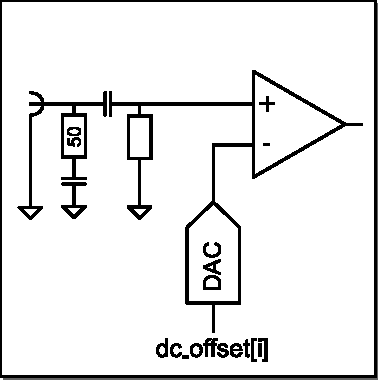
\includegraphics[width=0.3\textwidth]{xhptdc/figures/InputCircuit.pdf}
			}{
				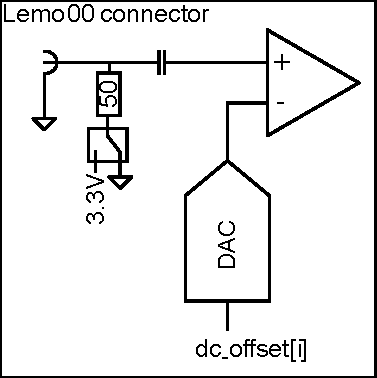
\includegraphics[width=0.3\textwidth]{figures/InputCircuit.pdf}
			}
			\caption{Input circuit for each of the input channels. \label{fig:dcoffset1}}
		\end{center} 
	\end{figure}
%%			\begin{figure}
%%				\begin{center}
%%					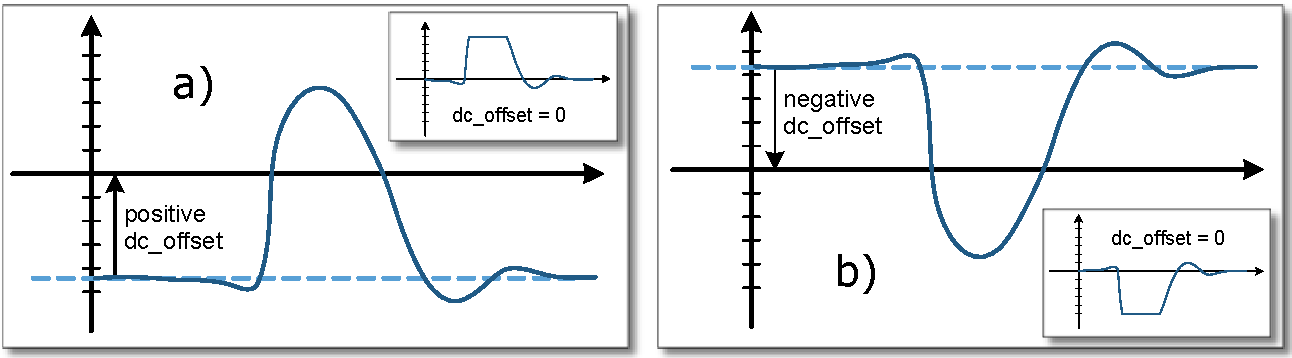
\includegraphics[width=\textwidth]{figures/dc_offset.pdf}
%%%					\caption{\textit{dc\tu offset} is used to shift the signal on each input channel such that the noise margin relative to the switching threshold is maximized.
%%					Insets of figure a) and b) show the base line of the signal with $\mathrm{\textit{dc\tu offset}}~=~0$ close to the switching threshold of the input buffer. Figure a) shows the positive pulse with $\mathrm{\textit{dc\tu offset}}~>~0$ and figure b) shows the negative pulse with $\mathrm{\textit{dc\tu offset}}~<~0$.\label{fig:dcoffset2}}
%%				\end{center}
%%			\end{figure}

	\ttvar{\prefix trigger}{trigger[\PREFIX TRIGGER\tu COUNT]}\\
	Configures the polarity of the external trigger sources.
	These are used as inputs for the TiGer blocks and as inputs to the time measurement unit.\par

	\ttvar{\prefix tiger\tu block}{tiger\tu block[\PREFIX TIGER\tu COUNT]}\\
	Configuration of the timing generators (TiGer).

	\ifxHPTDC{
		\ttvar{\prefix tiger\tu block}{gating\tu block[\PREFIX GATE\tu COUNT]}\\
		Configuration of the gating blocks.	
	}{} % only for xHPTDC8

	\ttvar{\prefix channel}{channel[\PREFIX CHANNEL\tu COUNT]}\\
		Configure the TDC channels.

	\ifxHPTDC{
		\cronvar{crono\tu bool\tu t}{skip\tu alignment}\\
		If set,  the phase of the two TDC chips is not realigned when capturing is restartet.

		\cronvar{crono\tu bool\tu t}{alignment\tu source}\\
		Define a signal source that is used for phase alignment. Should usually be left unchanged.
		\begin{tabular}{ll}
			\ttdef{ALIGN\tu TIGER} & 0\\
			\ttdef{ALIGN\tu PIN} & 1\\
			\ttdef{ALIGN\tu RESERVED} & 2\\
		\end{tabular}\par
		
	}{
		\ttvar{\prefix low-res\tu channel}{low-res\tu channel[\PREFIX LOWRES\tu CHANNEL\tu COUNT]}\\
		\itett{
			Not applicable for \deviceName. 
		}{
			Only applicable to the xTDC4-Sciex. Configures the additional digital low-res inputs.
		}\par
		\autotrigger
	
	}

	

%%%%%%%%% trigger
	\subsection{Structure \prefix trigger}
	\label{structtrigger}
	For each input this structure determines wheter rising or falling edges on the inputs create trigger events for the TiGer \ifxHPTDC{and gating}{} blocks.

	\cronvar{crono\tu bool\tu t}{falling}\\
	\cronvar{crono\tu bool\tu t}{rising}\\
	Select for which edges a trigger event is created inside the FPGA.
	\txh{
		Set the corresponding flag for one of the edges or both edges then using the input with a TiGer.
	}{
		The \deviceName can output measurements with a reduced bin size of $5/6~ns = 833,\overline{3}~ps$ for one or both edges of input signals. 
		See section \ref{difficulthits} for more information on hits with varying resolution.
		Use \textsf{xtdc4\tu channel.rising} on page \pageref{structchannel} to select which edge is measured with full resolution.
		The edge that is selected for full resolution measurement must also be enabled for low resolution measurement.
	}{
		While the TDC can only measure either rising or falling edges, the gating blocks and the TiGer are more flexibel. 
		Set the corresponding flag for one of the edges or both edges when using the input with a TiGer or gating block.
	}\par

%%%%% tiger_block			

	\subsection{Structure \prefix tiger\tu block\label{cp:tigerblock}}
	See section \ref{cp:tiger} for additional information.
	\ifxHPTDC{
		\cronvar{int}{mode}\\*
		Enables the desired mode of operation for the tiger. \\*
		\begin{tabular}{lrl}
			\ttdef{TIGER \tu OFF} & 0 & No operation \\
			\ttdef{TIGER \tu OUTPUT} & 1 & Output is driven with 2V amplitude. \\*
										&   &There must be no input connected \\
			\ttdef{TIGER \tu BIDI} & 2 & Output is driven with 1V amplitude. \\*
									&   & Pulse rate should be low. \\*
			\ttdef{TIGER \tu BIPOLAR} & 3 & Output is driven with 1~V bidirectional pulses.\\*
									&   & $start = stop -1$\\*
		\end{tabular}
		The gating blocks are only used internally and produce no pulses accessible to the user.		
		Gating blocks interpret any value that is not 0 as as enable.\\*
		\begin{tabular}{lrl}
			\ttdef{GATE \tu OFF} & 0 & No gating, alle hits are captured. \\*
			\ttdef{GATE \tu ON} & 1 & No hits are captured while the gate is active.\\*
		\end{tabular}
	
	}{
		\cronvar{crono\tu bool\tu t}{enable}\\
		Activates the timing generator (TiGer).\par
	}

	\cronvar{crono\tu bool\tu t}{negate}\\
	Inverts output polarity. Default is set to false.
	\ifxHPTDC{For gating blocks, a value of false blocks inputs between start and stop, a value of true blocks outputs outside that interval.
	The TiGer creates a high pulse from \textsf{start} to \textsf{stop} unless negated.}{}\par

	\cronvar{crono\tu bool\tu t}{retrigger}\\
	Enables retrigger setting.\\
	If enabled the timer is reset to the value of the \textsf{start} parameter, whenever the input signal is set while waiting to reach the \textsf{stop} time.\par

	\cronvar{crono\tu bool\tu t}{extend}\\
	Not implemented.

	\ifxHPTDC{}{
		\cronvar{crono\tu bool\tu t}{enable\tu lemo\tu output}\\
		Enables the LEMO output. Drive the TiGer Signal to the corresponding Lemo connector as an output. 
		This is DC coupled, so make sure that you do not any devices connected as inputs.
		Pulses created by the TiGer are visible at the \deviceName inputs and can be measured again to get the exact timing.  
	}

	\cronvar{int}{start}\\
	\cronvar{int}{stop}\\
	\itett{
		In multiples of $4~ns$.
	}{
		In multiples of $20~ns/3 = 6,\overline{6}~ns$
	}
	The time during which the TiGer output is set, relative to the trigger input. The parameters \textsf{start} and \textsf{stop} must fulfill the following conditions:
	\[ 0 <= start <= stop <= 2^{16}-1 \]
	If retriggering is enabled, the timer is reset to the value of the start parameter whenever the input signal is set while waiting for the stop time. \par
	

	\cronvar{int}{sources}\\
	A bit mask with a bit set for all trigger sources that can trigger this TiGer block. 
	Default is \textsf{\PREFIX TRIGGER\tu SOURCE\tu \ifxHPTDC{A}{S}}.\par

	\begin{tabular}{lc}
			\ttdef{TRIGGER\tu SOURCE\tu NONE} & 0x00000000\\
		\ifxHPTDC{
			\ttdef{TRIGGER\tu SOURCE\tu A} & 0x00000001\\
			\ttdef{TRIGGER\tu SOURCE\tu B} & 0x00000002\\
			\ttdef{TRIGGER\tu SOURCE\tu C} & 0x00000004\\
			\ttdef{TRIGGER\tu SOURCE\tu D} & 0x00000008\\
			\ttdef{TRIGGER\tu SOURCE\tu E} & 0x00000010\\
			\ttdef{TRIGGER\tu SOURCE\tu F} & 0x00000020\\
			\ttdef{TRIGGER\tu SOURCE\tu G} & 0x00000040\\
			\ttdef{TRIGGER\tu SOURCE\tu H} & 0x00000080\\
			\ttdef{TRIGGER\tu SOURCE\tu TDC1\tu SYNC} & 0x00000100\\
			\ttdef{TRIGGER\tu SOURCE\tu TDC2\tu SYNC} & 0x00000200\\
			\ttdef{TRIGGER\tu SOURCE\tu TDC\tu EXT\tu SYNC} & 0x00000400\\
			\ttdef{TRIGGER\tu SOURCE\tu ADC1\tu CONV} & 0x00000800\\
			\ttdef{TRIGGER\tu SOURCE\tu ADC2\tu CONV} & 0x00001000\\
			\ttdef{TRIGGER\tu SOURCE\tu AUTO} & 0x00004000\\
			\ttdef{TRIGGER\tu SOURCE\tu ONE}  & 0x00008000	
		}{
				\ttdef{TRIGGER\tu SOURCE\tu S} & 0x00000001\\
				\ttdef{TRIGGER\tu SOURCE\tu A} & 0x00000002\\
				\ttdef{TRIGGER\tu SOURCE\tu B} & 0x00000004\\
				\ttdef{TRIGGER\tu SOURCE\tu C} & 0x00000008\\
				\ttdef{TRIGGER\tu SOURCE\tu D} & 0x00000010\\
				\ttdef{TRIGGER\tu SOURCE\tu AUTO} & 0x00004000\\
				\ttdef{TRIGGER\tu SOURCE\tu ONE} & 0x00008000
		}
	\end{tabular} 

%%%%%%%%%%%%%%%%%%%%%%%% channel

	\subsection{Structure \prefix channel}
		\label{structchannel}
		Contains TDC channel settings.\par

		\cronvar{crono\tu bool\tu t}{enable\ifxHPTDC{}{d}}\\
		Enable TDC channel.\par

		\cronvar{crono\tu bool\tu t}{rising}\\
		\txh{
			Not applicable for \deviceName.
		}{
			Select which edge of the signal is used for full resolution measurements. 
			\textsf{xtdc4\tu trigger.rising} and \textsf{xtdc4\tu trigger.falling} described on page \pageref{structtrigger} are used 
			to select which edges are recorded for low resolution measurement. 
			The edge that is selected for full resolution measurement must also be enabled for low resolution measurement.
			See section \ref{difficulthits} for more information on hits with varying resolution.
		}{
			Select which edge of the signal is measured by the TDC. 
			The TiGer and gating blocks use a separate configuration that allows to use both edges simultaneously on each input. See section \ref{structtrigger}
		}\par

		\txh{}{ %only for xTDC4
			\cronvar{crono\tu bool\tu t}{cc\tu enable}\\
			Enable carry chain TDC. This is set to \emph{true} by default and should be left unchanged. \par

			\cronvar{crono\tu bool\tu t}{cc\tu same\tu edge}\\
			Sets whether the carry chain TDC records the same or opposite edge as the TDC chip. 
			If the same edge is selected, that carry chain TDC acts  as a backup if the chip misses hits due to FIFO overflows or short input pulses.
			If opposite edges are selected, both edges of a pulse can be measured with reasonable resolution. See section \ref{difficulthits} for more information.\par

			\cronvar{crono\tu bool\tu t}{ths788\tu disable}\\
			Disable full resolution timestamps. This is set to \emph{false} by default and should be left unchanged.\par
		}{}

		\ifxHPTDC{}{
			\cronvar{int}{start}\\
			\cronvar{int}{stop}\\
			Veto function for grouping of hits into packets in multiples of the binsize. Only hits between start and stop are read out.
			The parameters must adhere to the following relations:
			\[
				0 <= start <= stop < 2^{ \itett{31}{30}}
			\]
		}

%%%%%%%%%%%%%%%%%%%%% grouping, only fpr xHPTDC8

\ifxHPTDC{
	\subsection{Structure \prefix grouping\tu configuration}	
	\label{structgrouping}
	This structure configures the behaviour of the grouping functionality. See section \ref{grouping}.
	Grouping is enabled with the \textsf{tdc\tu mode} paramter defined in the top level of the config structure.

	In this structure intervals are always provided in picoseconds, independently of the bin size of the TDC.

	\cronvar{bool}{enable}
	Enable grouping. Defaults to \textsf{false}.

	\cronvar{int}{trigger\tu channel}\\
	Channel number that is used to trigger the creation of a group.\par

	\cronvar{int}{zero\tu channel}\\
	Optionally a different channel can be used to calculate the relative timestamps in a group. 
	This is disabled per default by setting this paramteer to $-1$.\par
	
	\cronvar{\tu\tu int64}{zero\tu channel\tu offset}\\
	This offset in picoseconds is added to relative timestamps within a group.\par

	\cronvar{\tu\tu int64}{range\tu start}\\
	\cronvar{\tu\tu int64}{range\tu stop}\\
	Values in the interval from \textsf{range\tu start} to \textsf{range\tu stop} are included in the group. 
	Either or both values can be negative to create common-stop behaviour. 
	\[
		-2^{63} \le range\_start \le range\_stop < 2^{63} 
	\]\par

	\cronvar{\tu\tu int64}{trigger\tu deadtime}\\
	After a trigger was detected additional triggers will be suppressed for this interval. Must not be negative.\par

	\cronvar{crono\tu bool\tu t}{require\tu windows\tu hit}\\
	If set a group is only created if there is at least one hit in the window defined by \textsf{window\tu start} and \textsf{window\tu stop}.\par

	\cronvar{\tu\tu int64}{window\tu start}\\
	\cronvar{\tu\tu int64}{window\tu stop}\\
	\[
		-2^{63} \le window\_ start \le window\_ stop < 2^{63} 
	\]\par

	\cronvar{int}{veto\tu mode}\\
	A window defined by \textsf{veto\tu start} and \textsf{veto\tu stop} can be used to suppress hits. 
	The functionality is very similar to the gating blocks but is defined in software. 
	While gating blocks can only work locally on the information available within each board the veto function is applied globally accross all boards.
	This feature can not be used to improve FIFO usage or PCIe bandwidth usage. 
	 \\*
	Either data inside or outside the veto window can be suppressed.\\*
	\begin{tabular}{lc}
		\ttdef{VETO\tu OFF}     & 0 \\
		\ttdef{VETO\tu INSIDE}  & 1 \\
		\ttdef{VETO\tu OUTSIDE} & 2 \\
	\end{tabular}\par

	\cronvar{\tu\tu int64}{veto\tu start}\\
	\cronvar{\tu\tu int64}{veto\tu stop}\\
	\[
		-2^{63} \le veto\_ start \le veto\_ stop < 2^{63} 
	\]\par

	\cronvar{crono\tu bool\tu t}{veto\tu relative\tu zero}\\
	If set, the veto window is defined relative to the zero channel. Otherwise the window is defined relative to the trigger.\par 

	\cronvar{crono\tu bool\tu t}{overlap}\\
	Unsupported, must remain \textsf{false}.

}{}



	
  
		  
	\chapter{Run Time Control\label{cp:readout}}  % and packet format
		\ifxHPTDC{
				%%%%%%%%%%%%%%%%% run time control
	\section{Controlling the State of the Driver}
	Once the devices are configured the following functions can be used to control the behaviour of the devices. 
	All of these functions return quickly with very little overhead, but they are not guaranteed to be thread safe.

		\ttvar{int}{start\tu capture(}\device)\\
		Start data acquisition.\par

		\ttvar{int}{pause\tu capture(}\device)\\
		Pause a started data acquisition. 
		Pause and continue have less overhead than start and stop but don't allow for a configuration change.\par

		\ttvar{int}{continue\tu capture(}\device)\\
		Call this to resume data acquisition after a call to \textsf{\prefix pause\tu capture()}.
		Pause and continue have less overhead than start and stop but don't allow for a configuration change.\par

		\ttvar{int}{stop\tu capture(}\device)\\
		Stop data acquisition.\par

		\ttvar{int}{start\tu tiger(}\device, \cronvar{int}{index})\\
		\ttvar{int}{stop\tu tiger(}\device, \cronvar{int}{index})\\
		Start and stop the timing generator of an individual board. 
		This can be done independently of the state of the data acquisition.\par	


\section{Readout}

\ttvar{int}{read\tu hits(}\device,  \cronvar{TDCHit}{*hit\tu buf,} \cronvar{size\tu t}{size} )\\
Read a multitude of hits into a buffer provided by the user. Returns the number of read hits.\\
If grouping is enabled a single group is read. 
If the group is to large for the buffer the remaining hits of the group are discarded.\\*
If grouping is disabled, all availabe data is read up to the size of the buffer. \\
The method always returns immediately. If no hits are read it of is beneficial to call \textsf{sleep()} 
or yield the CPU to another process instead of trying again immediately.\\
Make sure to set \textsf{size} to the number of elemenst that fit into the buffer.\\*

This function is not thread safe. 
If you want to process the read data in multiple threads the data needs to be copied to a seperate buffer for each thread.






		}{
			% NOTE: xHPTDC has a seperate file describing the readout

%%%%%%%%%%%%%%%%% run time control
\section{Run Time Control}
	\ttvar{int}{start\tu capture(}\device)\\
	Start data acquisition.\par

	\ttvar{int}{pause\tu capture(}\device)\\
	Pause a started data acquisition. 
	Pause and continue have less overhead than start and stop but don't allow for a configuration change.\par

	\ttvar{int}{continue\tu capture(}\device)\\
	Call this to resume data acquisition after a call to \textsf{\prefix pause\tu capture()}.
	Pause and continue have less overhead than start and stop but don't allow for a configuration change.\par

	\ttvar{int}{stop\tu capture(}\device)\\
	Stop data acquisition.\par

	\ttvar{int}{start\tu tiger(}\device)\\
	Start timing generator. This can be done independently of the state of the data acquisition.\par

	\ttvar{int}{stop\tu tiger(}\device)\\
	Stop timing generator. This can be done independently of the state of the data acquisition.\par

%%%%%% readout
\section{Readout}
	\ttvar{int}{acknowledge(}\device, \cronvar{crono\tu packet}{*packet)}\\
	Acknowledges the processing of the last read block. This is only necessary if \textsf{\prefix read()} is not called with 
	\textsf{in.acknowledge\tu last\tu read} set.\\
	This feature allows to either free up partial DMA space early if there will be no call to \textsf{\prefix read()} anytime soon. 
	It also allows to keep data over multiple calls to \textsf{\prefix read()} to avoid unnecessary copying of data. \par

	\ttvar{int}{read(}\device \cronvar{\prefix read\tu in}{*in,} \\ \cronvar{\prefix read\tu out}{*out)}\\
	Return a pointer to an array of captured data in \textsf{read\tu out}. 
	The result can contain any number of packets of type \textsf{\prefix packet}.
	\textsf{read\tu in} provides parameters to the driver. 
	A call to this method automatically allows the driver to reuse the memory returned in the previous call if \textsf{read\tu in.acknowledge\tu last\tu read} is set.\\
	Returns an error code as defined in the structure \textsf{\prefix read\tu out}.

	\subsection{Input Structure \prefix read\tu in}

		\ttvar{\prefix bool\tu t}{acknowledge\tu last\tu read}\\
		If set \textsf{\prefix read()} automatically acknowledges packets from the last read. 
		Otherwise \textsf{\prefix acknowledge()} needs to be called explicitely be the user. 

	\subsection{Input Structure \prefix read\tu out}
		\cronvar{crono\tu packet}{*first\tu packet}\\
		Pointer to the first packet that was captureed by the call of \textsf{\prefix read()}.\par

		\cronvar{crono\tu packet}{*last\tu packet}\\
		Address of header of the last packet in the buffer.\par

		\cronvar{int}{error\tu code}\\
		Assignments of the error codes.\par
		\begin{tabular}{lc}
			\crondef{CRONO\tu READ\tu OK} & 0\\
			\crondef{CRONO\tu READ\tu NO\tu DATA} & 1\\
			\crondef{CRONO\tu READ\tu INTERNAL\tu ERROR} & 2\\
			\crondef{CRONO\tu READ\tu TIMEOUT} & 3\par
		\end{tabular}\par

		\cronvar{const char}{*error\tu message}
		The last error in human readable form, possibly with additional information on the error.

	
		} 

	\chapter{Output Data Format\label{cp:packetformat}} 
		\ifxHPTDC{
			For each measured edge the \deviceName\ creates a 12 byte data structure TDCHit that contains a 64 bit timestamp in picoseconds and three fields with additional information. 

\section{Structure TDCHit}
\label{TDCHit}
\cronvar{long long}{time}\\
The time stamp of the hit in picoseconds. 

If grouping is disabled the timestamps are continuously counting up from the call to \textsf{start\tu capture()}.

If grouping is enabled the timestamps are relative to the trigger or the separate zero reference of the group. 
The first of a group has channel number 255 and provides the absolute time of the group. 
The absolute time of each of the hits can be obtained by adding this value to each of the relative timestamps.

\cronvar{unsigned char}{channel}\\
For the first board in the system this is 0 to 7 for the TDC channels A to H. 8 or 9 for ADC data. Data from channels 8 and 9 should usually be treated as data from the same channel. 
For the other boards the channel number is incremented by $board\_id \cdot 10$.
In grouping mode the first hit of each group has channel number 255 and contains the absolute time of the group.

\cronvar{unsigned char}{type}\\
Additional information on the type of hit recorded. See section \ref{hittypes}.

\cronvar{unsigned short}{bin}\\
For ADC hits this contains the sampled voltage. For TDC hits the content is undefined.

\newpage
\subsection{TDCHit Types \label{hittypes}}
\newcommand{\HTYPE}{\PREFIX TDCHIT\tu TYPE\tu}

\paragraph*{Type information for TDC measurements}
If the hit is a TDC measurement on channels A to H the following flags are defined for the \textsf{type} field of the TDCHit structure:\\*
\begin{tabular}{lc}
    \crondef{\HTYPE RISING} & 0x01\\
    \indent Rising edge &\\
    \crondef{\HTYPE ERROR}  & 0x02\\
    \indent any type of error& \\
    \crondef{\HTYPE ERROR\tu TIMESTAMP\tu LOST}  & 0x04\\
    \indent Hits missing due to L1 FIFO overflow&\\
    \crondef{\HTYPE ERROR\tu ROLLOVER\tu LOST}  & 0x08\\
    \indent Invalid timestamp due to internal error&\\
    \crondef{\HTYPE ERROR\tu PACKET\tu LOST}  & 0x10\\
    \indent Hits missing due to a lost DMA packet&\\
    \crondef{\HTYPE ERROR\tu SHORTENED}  & 0x20\\
    \indent Hits missing due to a shortened DMA packet&\\
    \crondef{\HTYPE ERROR\tu DMA\tu FIFO\tu FULL}  & 0x40\\
    \indent Hits missing due to L2 FIFO overflow&\\
    \crondef{\HTYPE ERROR\tu HOST\tu BUFFER\tu FULL}  & 0x80\\
    \indent Hits missing due to host buffer overflow &\\
\end{tabular}

If hits are missing the error flag is set on the next hit from the same board that is read out.

\paragraph*{Type information for ADC measurements}
If the hit is an ADC measurement on channels 8 or 9 the following flags are defined for the \textsf{type} field of the TDCHit structure:\\*
\begin{tabular}{lc}
    \crondef{\HTYPE ADC\tu INTERNAL} & 0x01\\
    \indent ADC measurement triggered by TiGer &\\
    \crondef{\HTYPE ADC\tu ERROR}  & 0x02\\
    \indent any type of error& \\
    \crondef{\HTYPE ADC\tu ERROR\tu INVALID\tu TRIGGER}  & 0x08\\
    \indent TRG input violated timing requirements. Data may be corrupted&\\
    \crondef{\HTYPE ADC\tu ERROR\tu DATA\tu LOST}  & 0x10\\
    \indent ADC measurement missing due to overflow of any buffer&\\
\end{tabular}

If hits are missing the error flag is set on the next hit from the same board that is read out.


 
		}{
			


\section{Output Structure crono\tu packet}

	\cronvar{unsigned char}{channel}\\
	Unused, always 0.\par

	\cronvar{unsigned char}{card}\\
	Identifies the source card in case there are multiple boards present. Defaults to 0 if no value is assigned to the parameter \textsf{board\tu id} in Structure \textsf{ndigo\tu init\tu parameters}.\par

	\cronvar{unsigned char}{type}\\
	The data stream consists of 32-bit unsigned data as signified by a value of 6.\par

	\cronvar{unsigned char}{flags}\\
	\indent\ttdef{ PACKET\tu FLAG\tu ODD\tu HITS} 1\\
	\indent The last data word in the data array consists of one timestamp only which is located in the lower 32 bits of the 64-bit data word (little endian).\par
	\indent\ttdef{ PACKET\tu FLAG\tu SLOW\tu SYNC} 2\\
	\indent Start pulse distance is larger than the extended timestamp counter range.\par
	\indent\ttdef{ PACKET\tu FLAG\tu START\tu MISSED} 4\\
	\indent The trigger unit has discarded packets due to a full FIFO.\par
	\indent\ttdef{ PACKET\tu FLAG\tu SHORTENED} 8\\
	\indent The trigger unit has shortened the current packet due to full FIFO.\par
	\indent\ttdef{ PACKET\tu FLAG\tu DMA\tu FIFO\tu FULL} 16\\
	\indent The internal DMA FIFO was full. Might or might not result in dropped packets.\par
	\indent\ttdef{ PACKET\tu FLAG\tu HOST\tu BUFFER\tu FULL} 32\\
	\indent The host buffer was full. Might or might not result in dropped packets.\par

	\cronvar{unsigned int}{length}\\
	Number of 64-bit elements (each containing up to 2 TDC hits) in the data array.\par

	\cronvar{unsigned \tu\tu int64}{timestamp}\\
	Coarse timestamp of the start pulse. Values are given in multiples of \itett{$500$~ps}{$5/3=1.\overline{6}$~ns}.\par

	\cronvar{unsigned \tu\tu int64}{data[1]}\\
	TDC hits. the user can cast the array to uint32* to directly operate on the TDC hits.

	\noindent
	\begin{small}
	\begin{tabular}{|c||p{9cm}|p{1,5cm}|p{1,5cm}|}
		\hline
		bits & 31~ ~ ~ ~ ~ ~ ~ ~ ~ ~ ~ ~ ~ ~ ~ ~ ~ to ~ ~ ~ ~ ~ ~ ~ ~ ~ ~ ~ ~ ~ ~ ~ ~ ~ 8 & 7~ ~ to ~ ~ 4 & 3~ ~ to ~ ~ 0\\\hline
		content & TDC DATA & FLAGS & CHN \\\hline
	\end{tabular}
	\end{small}

	The timestamp of the hit is stored in bits 31 down to 8 in multiples of 
	\itett{500~ps. For the -1G Variant bit 8 is always 0.}{
		$5/(3*128) = 13.0208\overline{3}$~ps
	}\\
	
	\label{flags}
	Bits 7 down to 4 are hit flags:\par
	\itett{
		Bit 7: Always 0.\par
		Bit 6: Always 1.\par
	} {
		Bit 7, 6: Resolution of this measurement. \ifxHPTDC{}{See section \ref{difficulthits}}.\\
		\noindent
		\begin{small}
		\begin{tabular}{|c|c||l|}
			\hline
			bit 7 & bit 6 & Measurement Type \\\hline\hline
			0 & 0 &  Normal full resolution measurement.\\\hline
			0 & 1 &  Measurement performed with carry chain TDC at about 150~ps resolution.\\\hline
			1 & 0 &  Full resolution measurement that might in the wrong place in the data stream.\\\hline
			1 & 1 &  Measurement with only $5/6~ns = 833.\overline{3}~ps$ resolution. \\\hline
		\end{tabular}
		\end{small}
		
	}
	Bit 5: Rollover. The time since start pulse exceeded the \itett{23}{24}-bit range that can be ecnoded in a data word. This word does not encode a measurement. 
	Instead the readout software should increment a rollover counter that can be used as the upper bits of consecutive time stamps.  
	The counters should be reset for each packet.
	The total offset of a hit in picoseconds can be computed by
	\[	\Delta T_{hit} = \mathrm{(\#\ rollovers \cdot 2^{\itett{23}{24}} + TDC\_ DATA_{hit}) \cdot \itett{timetagger4}{xtdc4}\_param\_info.binsize} \]
	\indent
	Bit 4: Set if this word encodes a rising edge. Otherwise, this word belongs to a falling edge.
	The channel number is given in the lowest nibble of the data word. A value of 0 corresponds to channel A, a value of 3 to channel D.\par
 
		}  
 
	\chapter{Code Example}  
		% SVN Info:
% $Date: 2021-01-31 20:06:56 +0100 (So, 31 Jan 2021) $
% $Rev: 1040 $
% $Author: kolja $

	The following C++ source code shows how to initializes a \deviceName\ board, configure it and loop over incoming packets.	

	If you are reading this documentation in portable document format, the source code of the C example is also embedded as an
	\txh{
		\textattachfile[color=cronlightgreen, description={Example Source Code}]{"timetagger/example.cpp"}{attachment}
		to the file. You can open it in an external viewer or save it to disk by clicking on it.
		\lstinputlisting{timetagger/example.cpp}
	}{
		\textattachfile[color=cronlightgreen, description={Example Source Code}]{xtdc/example.cpp}{attachment}
		to the file. You can open it in an external viewer or save it to disk by clicking on it.
		\lstinputlisting{xtdc/example.cpp}
	}{	
		\textattachfile[color=cronlightgreen, description={Example Source Code}]{xhptdc/example.cpp}{attachment}
		to the file. You can open it in an external viewer or save it to disk by clicking on it.

		The example code is managed as open source on GitHub at 
		\href{https://github.com/cronologic-de/xhptdc8_babel/tree/main/ug_example}{https://github.com/cronologic-de/xhptdc8\tu babel}. 
		The repository contains a complete project for Microsoft Visual Studio that you can use to compile the example.
		Examples for more programming languages such as Golang, Rust, Python and LabView will be added to the repository over time.

		At the time this document is written, the following source code can be found in the repository:
		\begin{itemize}
			\item \href{https://github.com/cronologic-de/xhptdc8_babel/tree/main/dummy}{dummy library} to be able to develop code for the \deviceName\ without a physical board beeing present
			\item \href{https://github.com/cronologic-de/xhptdc8_babel/tree/main/util}{utility library} to configure the device from YAML strings or YAML files 
			\item command line info tool to list information about all \deviceName\ boards in the system. This tool is written in Go.
		\end{itemize}

		\lstinputlisting{xhptdc/example.cpp}
	}
	% there were problems with underscores in file names so we removed them



	\chapter{Technical Data}    
		\ttinput{Tech.tex} 
		% SVN Info:
% $Date: 2021-01-29 22:28:41 +0100 (Fr, 29 Jan 2021) $
% $Rev: 1039 $
% $Author: kolja $
\section{Electrical Characteristics}

	\subsection{Power Supply}

		\noindent
		\begin{tabularx}{\textwidth}{|c|X|c|c|c|c|}
			\hline
			Symbol & Parameter & Min & Typical & Max & Units\\
			\hline\hline
			P & Total power consumption &&& 25& W\\
			\hline
			I & PCIe 3,3V rail input current &&&4& mA\\
			\hline
			VCC & PCIe 3,3V rail power supply voltage &3,1&3,3&3,5& V\\
			\hline
			I & PCIe 12V rail input current &&&2,1& A\\
			\hline
			VCC & PCIe 12V rail power supply voltage &11,1&12&12,9& V\\
			\hline
			I & PCIe 3,3VAux rail input current &&0&& A\\
			\hline
			VCC & PCIe 3,3VAux rail power supply voltage &&3,3&& V\\
			\hline
		\end{tabularx}

	\subsection{TDC Inputs}

		The \deviceName's inputs are single-ended AC-coupled with 50$\Omega$ DC termination.

		\noindent
		\begin{tabularx}{\textwidth}{|c|X|c|c|c|c|}
			\hline
			Symbol & Parameter & Min & Typical & Max & Units\\
			\hline\hline
			V\subscript{Base} & Input Baseline & 0 & & 5 & V\\
			\hline
			V\subscript{Threshold} & Trigger Level & V\subscript{Base} - 1.32 & & V\subscript{Base} + 1.18 & V\\
			\hline
			t\subscript{Pulse} & Pulse Length & 2 & 5 & 200 & ns\\
			\hline
			t\subscript{Rise} & Pulse Edge 20\% to 80\%  &  &  & 10 & ns\\
			\hline
			t\subscript{Fall} & Pulse Edge 80\% to 20\%  &  &  & 10 & ns\\
			\hline
			Z\subscript{P} & Input Impedance && 50 && $\Omega$\\
			\hline
			I\subscript{Term} & Termination Current & -50 & -20 & 50 & mA\\
			\hline
		\end{tabularx}

	All inputs are AC coupled. The inputs have very high input bandwidth requirements and therefore there are no circuits that provide over voltage protection for these signals. 
	Any voltage on the inputs above 5V or below -5V relative to the voltage of the slot cover can result in permanent damage to the board.
	
	\ifxHPTDC{
		All digital inputs can output AC coupled pulses from the TiGer. 
		Special care should be taken not to enable the TiGer output when sensitive equipment is connected that could be damaged by the pulses. 
	}{
		Make sure not to drive the inputs when the connector is configured as a TiGer output. 
	}
	See Section \ref{cp:tiger}. 
%%%%%%%%%%% ADC input
	\ifxHPTDC{
	\newpage
	\subsection{ADC Inputs}
	The ADC input is DC coupled to a differential termination voltage of 400~mV. 
	This means that the actual voltage seen by the ADC will depend on the output impedance of the source that is driving the input.\\*
	\noindent
		\begin{tabularx}{\textwidth}{|c|X|c|c|c|c|}
			\hline
			Symbol & Parameter & Min & Typical & Max & Units\\
			\hline\hline
			V\subscript{in} & Input voltage & -2.0 &  & 2.5 & V \\
			\hline 
			V\subscript{term} & Termination voltage & & 0.4 & & V \\
			\hline 
			Z\subscript{in} & Input Impedance & & 50  & & $\Omega$ \\
			\hline
		\end{tabularx}

%%%%%%%%%%% clock input		
	\subsection{Clock input J2}
	The ADC input is DC coupled to a differential termination voltage of 400~mV. 
	This means that the actual voltage seen by the ADC will depend on the output impedance of the source that is driving the input.\\*
	\noindent
		\begin{tabularx}{\textwidth}{|c|X|c|c|c|c|}
			\hline
			Symbol & Parameter & Min & Typical & Max & Units\\
			\hline\hline
			V\subscript{p-p} & Peak to Peak voltage & 1 &  & 3.3 & V \\
			\hline 
			V\subscript{cm} & Common mode voltage voltage &-3 & 0 & 3 & V \\
			\hline 
			V\subscript{tck} & Clock termination voltage & & 0 &  & V \\
			\hline 
			Z\subscript{in} & Input Impedance & & 50  & & $\Omega$ \\
			\hline 
			D\subscript{J2} & Duty cycle & 45 & 50 & 55 & \% \\
			 \hline 
			 f\subscript{J2}& Frequency &  & 10 &  & MHz \\
			\hline
		\end{tabularx}
}{}

\newpage
\section{Information Required by DIN EN 61010-1}
\subsection{Manufacturer\label{cp:manu}}

The \deviceName\ is a product of:\

\begin{quote}
	cronologic GmbH \& Co. KG\\
	Jahnstra\ss{}e 49\\
	60318 Frankfurt\par
	Germany
	\noindent HRA 42869 beim Amtsgericht Frankfurt/M\par
	\noindent VAT-ID: DE235184378
	\noindent PCI Vendor ID: 0x1A13
\end{quote}

\subsection{Intended Use and System Integration}

	The devices are not ready to use as delivered by cronologic. It requires the development of specialized software to fulfill the application of the end user. The device is provided to system integrators to be built into measurement systems that are distributed to end users. These systems usually consist of the \deviceName, a main board, a case, application software and possible additional electronics to attach the system to some type of detector. They might also be integrated with the detector.\par

	The \deviceName\ is designed to comply with DIN EN 61326-1 when operated on a PCIe compliant main board housed in a properly shielded enclosure. 
	When operated in a closed standard compliant enclosure the device does not pose any hazards as defined by EN 61010-1.\par

	Radiated emissions, noise immunity and safety highly depend on the quality of the enclosure. 
	It is the responsibility of the system integrator to ensure that the assembled system is compliant to applicable standards of the country that the system is operated in, especially with regards to user safety and electromagnetic interference. \par
	 
	When handling the board, adequate measures must be taken to protect the circuits against electrostatic discharge (ESD). All power supplied to the system must be turned off before installing the board.

	\subsection{Environmental Conditions for Storage}

	The board shall be stored between operation under the following conditions:

	\noindent
	\begin{tabularx}{\textwidth}{|c|X|c|c|c|c|}
		\hline
		Symbol & Parameter & Min & Typical & Max & Units\\
		\hline\hline
		T & ambient temperature & -30 && 60 & $^{\circ}$C\\
		\hline
		RH & relative humidity at 31$^{\circ}$C noncondensing & 10 && 70 & \%\\
		\hline
	\end{tabularx}


\subsection{Environmental Conditions for Operation}

	The board is designed to be operated under the following conditions:

	\noindent
	\begin{tabularx}{\textwidth}{|c|X|c|c|c|c|}
		\hline
		Symbol & Parameter & Min & Typical & Max & Units\\
		\hline\hline
		T & ambient temperature & 5 && 40 & $^{\circ}$C\\
		\hline
		RH & relative humidity at 31$^{\circ}$C & 20 && 75 & \%\\
		\hline
	\end{tabularx}

	WARNING: Do not connect any DC coupled inputs to a channel while the TiGer of that channel is configured as an output (see Section \ref{cp:tiger}).
	Doing so could do permanent damage to the \deviceName\ and the external hardware.

\subsection{Cooling}

	The \deviceName\ in its base configuration has passive cooling that requires a certain amount of air flow. 
	If the case design can't provide enough air flow to the board, a slot cooler like Zalman ZM-SC100 can be placed next to the board. 
	Active cooling is also available as an option for the board.


\subsection{Recycling}

	cronologic is registered with the ``Stiftung Elektro-Altger\"a{}te Register'' as a manufacturer of electronic systems with Registration ID DE 77895909.\par
	The \deviceName\ belongs to category 6, ``Kleine Geräte der Informations- und Telekommunikationstechnik für die ausschließliche Nutzung in anderen als privaten Haushalten''. 
	Devices sold before 2018 belong to category 9, ``\"U{}berwachungs und Kontrollinstrumente f\"u{}r aus\-schlie\ss lich gewerbliche Nutzung''. 
	
	The last owner of a \deviceName\ must recycle it, treat the board in compliance with \S{}11 and \S{}12 of the German ElektroG, or return it to the manufacturer's address listed on page \pageref{cp:manu}.
	

	\chapter{Revision History} 
		\noindent
		User Guide \hyperlink{ugrev}{\ugrev} as of 2020-04-13\\  %needs also be updated in UgRev.tex
		\\
		cronologic GmbH \& Co. KG\\
		Jahnstraße 49\\
		60318 Frankfurt am Main\\Germany\\
		\ttinput{FwRev.tex}
		\ifxHPTDC{\section{Driver \& Applications}
\begin{tabularx}{\textwidth}{|c|c|X|}
    \hline
    Revision & Date & Comments\\
    \hline\hline
    \hypertarget{drvrev}{0.x.x} & 2021 & preliminary driver\\
    \hline
 
\end{tabularx}}{\section{Driver \& Applications}
\begin{tabularx}{\textwidth}{|c|c|X|}
    \hline
    Revision & Date & Comments\\
    \hline\hline
    \hypertarget{drvrev}{1.4.1} & 2019-11-11 & x64 32 mode issues fixed\\
    \hline
    {1.4.0} & 2019-06-04 & Improved Windows 10 support\\
    \hline
    {1.3.0} & 2019-01-23 & Added Windows 10 support\\
    \hline
\end{tabularx}} 
		% Also update date and version in User_Guide.tex

\section{User Guide}
\begin{tabularx}{\textwidth}{|c|c|X|}
    \hline
    Revision & Date & Comments \\
    \hline\hline  
    \hypertarget{ugrev}{1.8.1} & 2021-04-09 &
    \makecell[l]{
        Many corrections and updates to the xHPTDC8 API.
    }\\
    \hline 
    {1.8.0} & 2021-03-22 &
    \makecell[l]{
        Added xHPTDC8 User Guide
    }\\
    \hline 
    {1.7.0} & 2021-02-04 & 
    \makecell[l]{
        Combined User Guide for -1G and -2G \\
        Added characteristics for INL, DNL and Time Base \\
        Reordered sections for clarity \\
        Error corrections for rollovers, binsize and range \\
        Added figure \ref{fig:matrix} (TiGer matrix) \\
        Corrected board revision \\
    }\\
    \hline
    \itett{1.3.0}{1.6.0} & 2019-06-05 & API clarifications \\
    \hline
\end{tabularx} 
\end{document}  